\documentclass{article}
\usepackage[backend=biber, citestyle=authoryear, bibencoding=utf8]{biblatex}
\addbibresource{./bibs/vlab-report.bib}
\usepackage{adjustbox}
\usepackage{graphicx}
\usepackage[utf8]{inputenc}
\usepackage{geometry}
\usepackage{lscape}
\usepackage{dcolumn}
 \geometry{
 a4paper,
 total={170mm,257mm},
 left=10mm,
 top=10mm
 }

\title{Bebbo}
\date{September 2023}

\begin{document}

\tableofcontents

% \section*{Executive Summary}

% We perform a randomized control trial in two countries, Serbia and Bulgaria, to determine the impact the parenting app Bebbo has on users across several outcomes of interest, covering knowledge, attitudes, and beliefs.

% Pre-exposure to the treatment in both of these countries was significant. 55\% knew about the app and 23\% reported having used it before. Treatment group takeup, new users of the app, was 28\%\footnote{we ae still verifying the validity of that number by confirming functionality of reporting with the app developers}, with 12\% using the app more than one day and 3\% using the app more than three days within the intervention period which lasted 4-6 weeks.

% Significant pre-exposure of the intervention implies that what is measured in this evaluation is the population impact of adding new and additional Bebbo users, beyond those who might have already existed. Note that new users may be different compared with old or ``early adopter'' users, which we cannot fully determine in this study. However, we will compare app usage data between the two groups to determine how similar they behave in app engagement.

% We measure effects on eight outcomes across three domains: knowledge, attitudes, and practices. We do not find any statistically significant impacts of the treatment, however, there are caveats based on study design:

% \begin{enumerate}
% \item We were reasonably powered (80\%) to find a medium effect size on a 28\% takeup, however, we were not able to detect a smaller effect size or a medium effect size on a smaller takeup group.
% \item Some of the items, particularly knowledge, seemed to suffer from a ``survey effect'' where answers improved from baseline to endline for all groups.
% \item Many of the outcome instruments suffered from ceiling effects, where large portions of the population scored a perfect score on the baseline and had no room for improvement. This reduces the ability to find a medium effect size on these outcomes.
% \end{enumerate}

% \subsection*{Knowledge}

% There is some suggestive evidence that knowledge of vaccines improves under treatment, while knowledge of child development did not seem impacted by treatment.

% 
% Table created by stargazer v.5.2.3 by Marek Hlavac, Social Policy Institute. E-mail: marek.hlavac at gmail.com
% Date and time: Sun, Feb 11, 2024 - 04:03:43 PM
\begin{table}[!htbp] \centering 
  \caption{Pooled: OLS - Endline - Knowledge and Awareness} 
  \label{tbl:Pooled: OLS - Endline - Knowledge and Awareness} 
\begin{tabular}{@{\extracolsep{5pt}}lcc} 
\\[-1.8ex]\hline 
\hline \\[-1.8ex] 
 & \multicolumn{2}{c}{\textit{Dependent variable:}} \\ 
\cline{2-3} 
\\[-1.8ex] & Vaccine Knowledge & Child Dev. Knowledge \\ 
\\[-1.8ex] & (1) & (2)\\ 
\hline \\[-1.8ex] 
 Treatment & 0.04 & $-$0.001 \\ 
  & (0.03) & (0.01) \\ 
  & & \\ 
\hline \\[-1.8ex] 
Adjusted Treatment p-value & 0.467 & 0.957 \\ 
Observations & 667 & 1,811 \\ 
R$^{2}$ & 0.01 & 0.01 \\ 
\hline 
\hline \\[-1.8ex] 
\textit{Note:}  & \multicolumn{2}{r}{$^{*}$p$<$0.1; $^{**}$p$<$0.05; $^{***}$p$<$0.01} \\ 
\end{tabular} 
\end{table} 


% When looking at raw pre-post data for each group, we see that our knowledge outcomes improved across all groups, regardless of treatment assignment or takeup (see figure \ref{fig:pre_post_knowledge}). This is consistent with the hypothesis that asking parents a question about their knowledge (i.e. ``Do you know which vaccine your child needs to take next?'') might cause them to go out and learn the answer before the next survey. There is some evidence that those who download and use the app are more likely to have expressed a lack of knowledge at baseline, indicating that those who need the knowledge are more likely to try the app.

% \begin{figure}[h!]
%   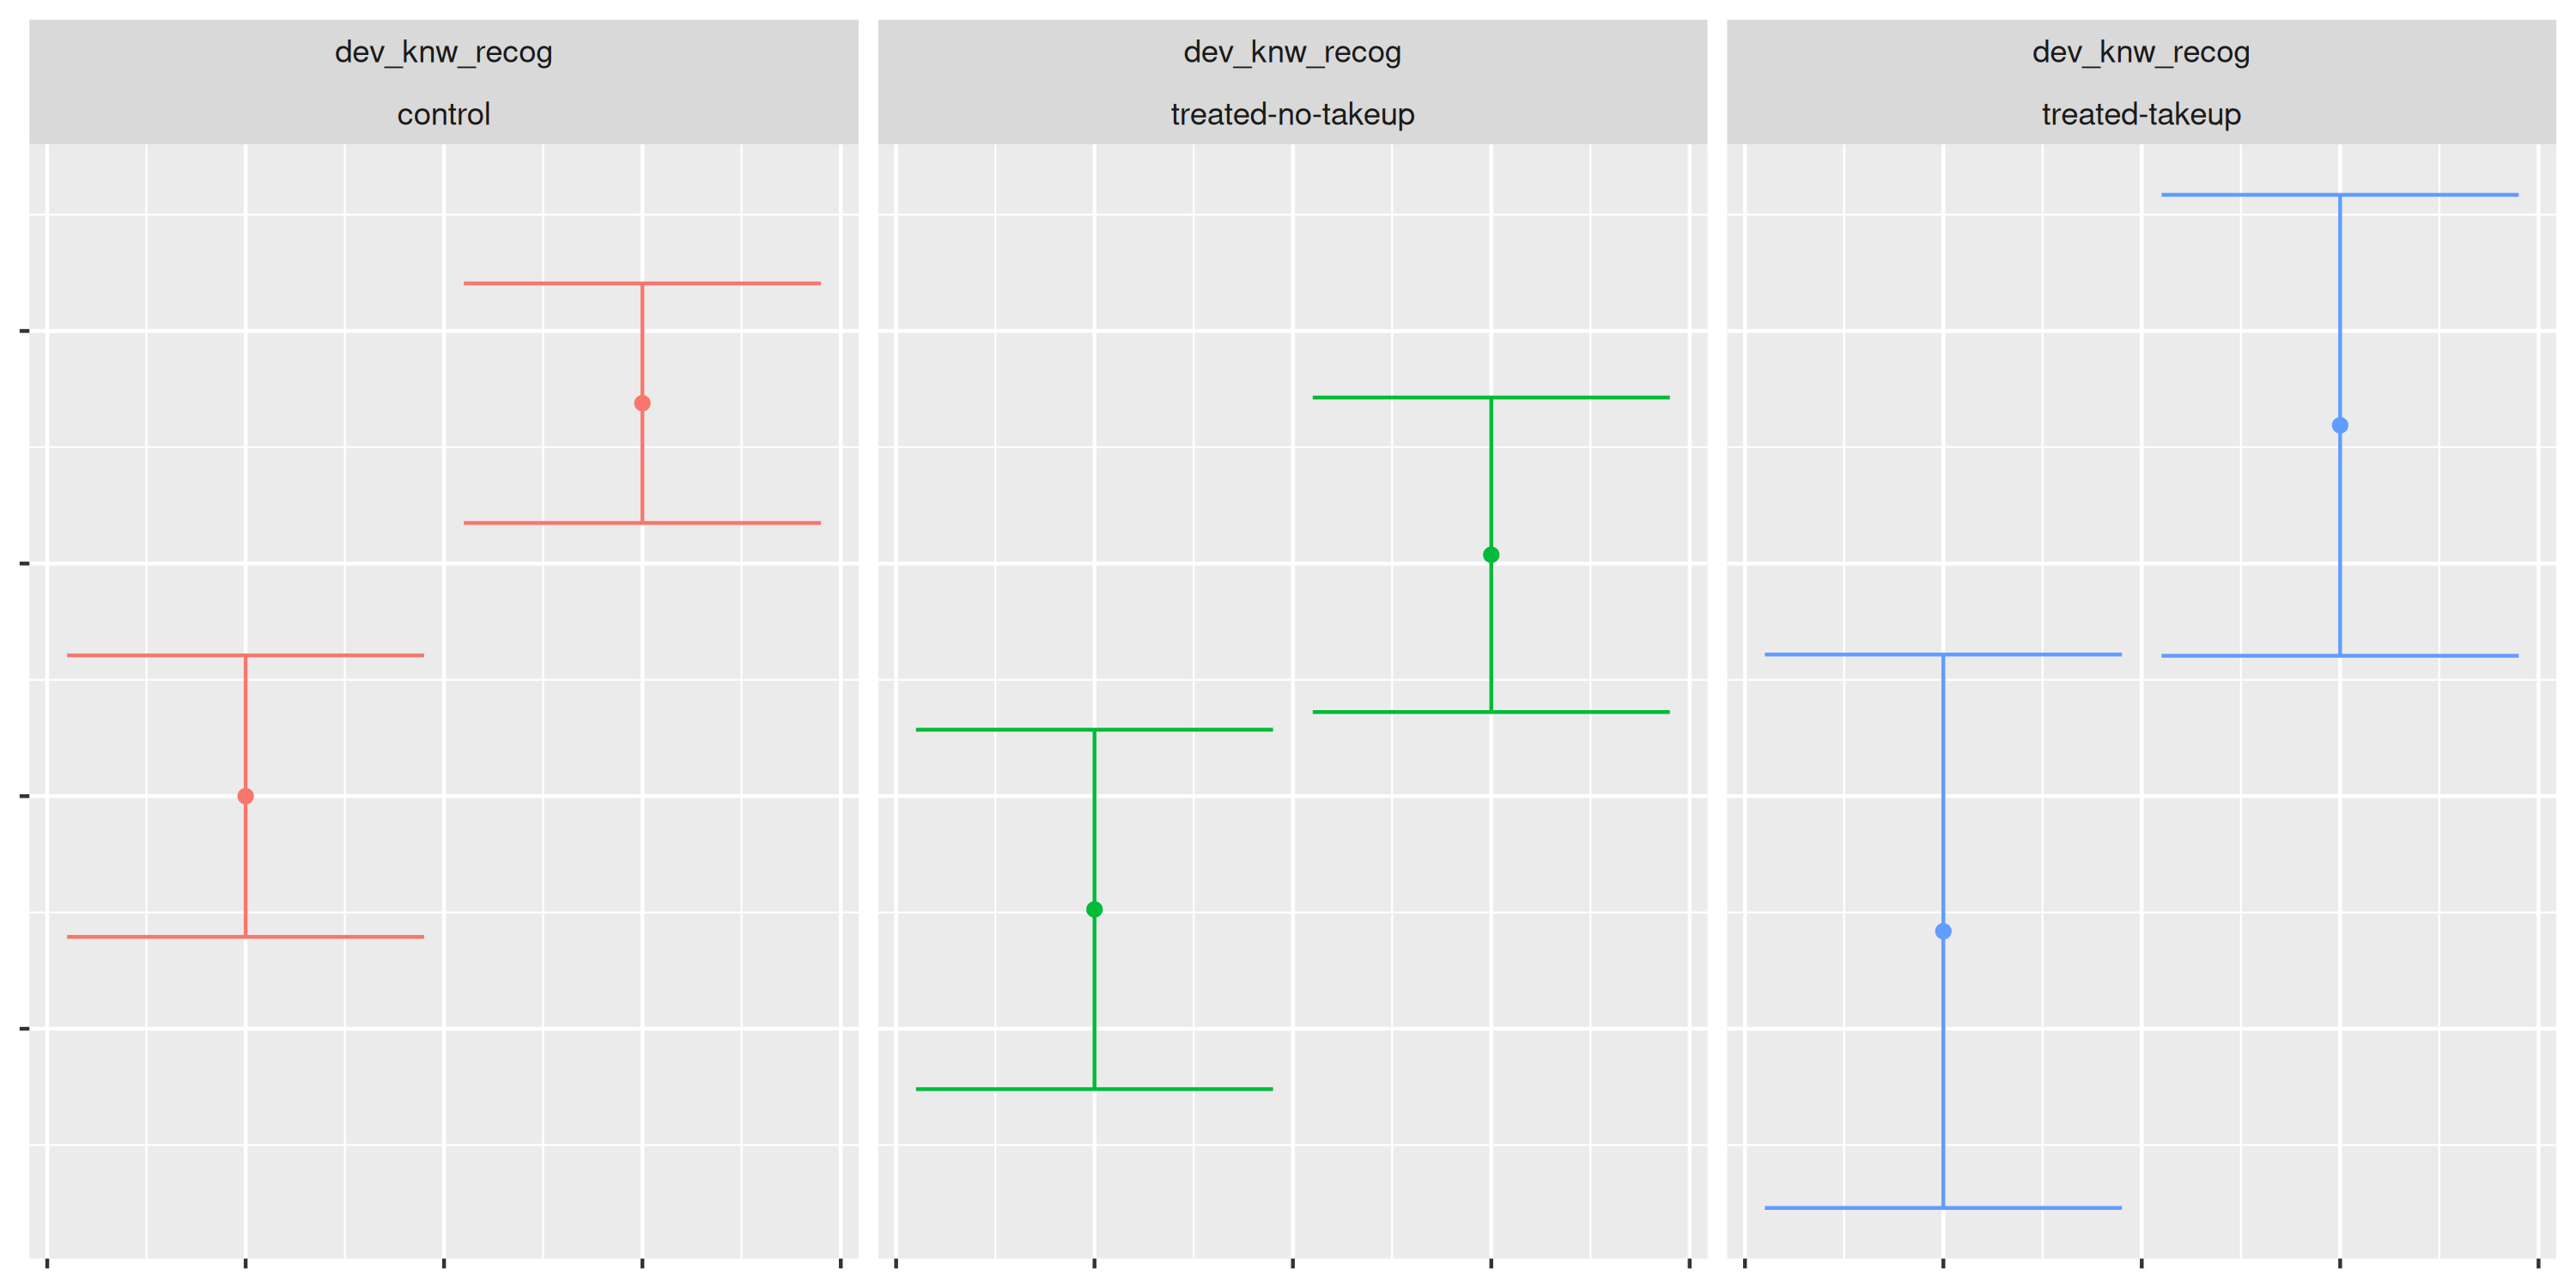
\includegraphics[width=\textwidth]{plots/pre_post/health_knw.png}
%   \caption{Raw Pre-Post Knowledge Outcome Data}
%   \label{fig:pre_post_knowledge}
% \end{figure}

% While the effect size is small and not significant, it is suggested by the point estimate that the app was more effective at helping participants learn about the next required vaccine than the control condition.

% \subsection*{Attitudes}

% There were no significant effects on parenting confidence or attitudes toward physical punishment. There is a small measured positive effect on attitude toward physical punishment in the regression, but this is driven by a negative movement among the control group, which is hard to justify or explain.

% There was some evidence that those who were less confident at baseline were more likely to use the app. However, there is no evident that the treatment condition was more effective than the control condition at increasing confidence, potentially driven by survey effects again where all conditions increased in confidence (see figure \ref{fig:pre_post_confidence}).


% \begin{figure}[h!]
% 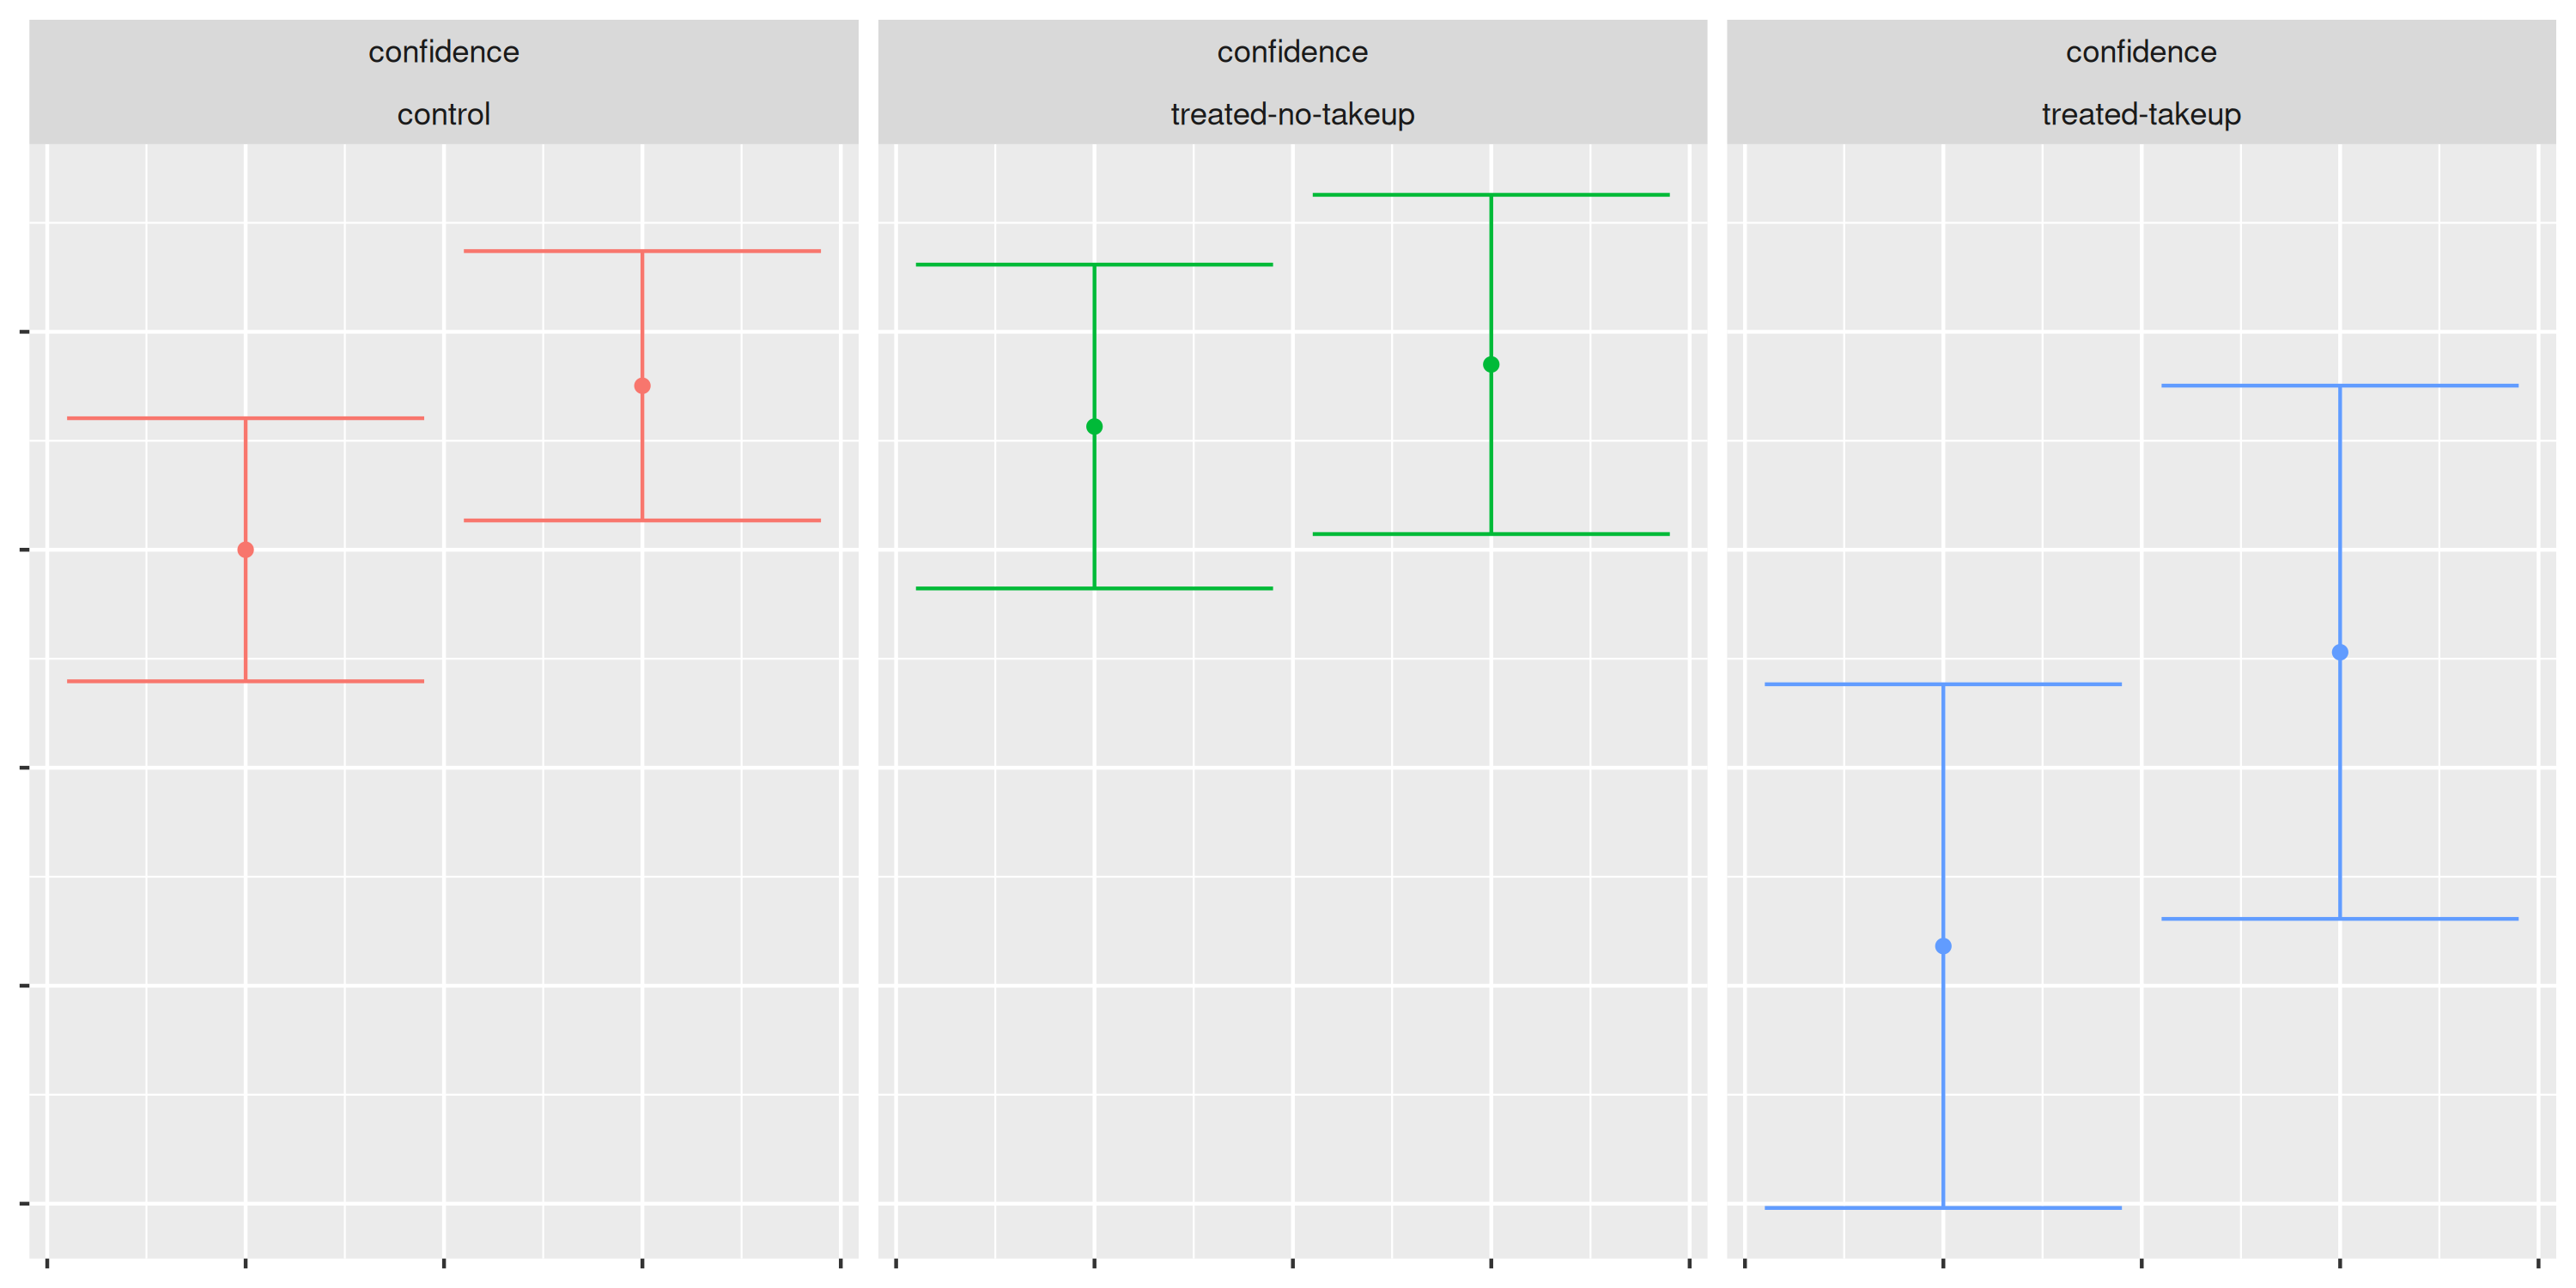
\includegraphics[width=\textwidth]{plots/pre_post/confidence.png}
%   \caption{Raw Pre-Post Knowledge Outcome Data}
%   \label{fig:pre_post_confidence}
% \end{figure}


% \subsection*{Practices}

% There were no significant effects measured on changes in practices. There is a small measured positive effect on ``Practices in the lsat 24 hours'', but this is primarily driven by those who did not download or use the app, which is also hard to explain. Similarly to others, there was a potential survey effect and all conditions saw an increase in this outcome.



% \clearpage
\section{Introduction}

\addcontentsline{toc}{subsection}{About Bebbo}
\subsection*{About Bebbo}
Parents everywhere are in need of information on various aspects of child development from reliable  and validated sources as well as guidance on how to support the health and development of their  children. However, services providing this sort of information and support are often non-existent or  inaccessible for a lot of parents in many places. Often, service providers, even when accessible, might  lack necessary knowledge and skills to respond to the questions and concerns parents might have.

Mobile apps are one of the most convenient and easy ways to access information about child  development and parenting. However, parenting apps are mainly in English and provide a limited  thematic content without a possibility for parents to familiarize with, track, and support all aspects of  their child’s health and development. In addition, these apps are, naturally, not adapted to contexts of  individual countries. Many apps are not free of charge, which presents a significant barrier, particularly  for the most vulnerable families. At the same time, the majority of the existing apps operate only in  online mode requiring good internet connectivity that is lacking in remote and rural areas.

To support parents to receive timely and quality guidance even when direct contact with service  providers is not possible and overcome barriers in access to localized digital solutions with verified  content, UNICEF Europe and Central Asia Regional Office (ECARO) developed a mobile parenting app,  Bebbo. The mobile application also supports the most vulnerable parents/caregivers with lower  education level, in terms of the navigation modalities, off-line operability and selection of the core  content. The two main objectives of Bebbo, in line with the UNICEF ECARO Early Childhood  Development Theory of Change, are: (1) Improving availability of information for parents on child  development, and (2) Supporting parents for responsive caregiving and early intervention.  Accordingly, Bebbo app provides users information and interactive tools to help nurture and aid their  child’s health and development. The launch of Bebbo in 11 countries in the ECA region is a direct  response to the identified objective to engage parents and caregivers in nurturing care, positive  parenting, stimulating, and learning.

\addcontentsline{toc}{subsection}{What question does this evaluation answer?}
\subsection*{What question does this evaluation answer?}
The design of the study is set up to answer the following question in the positive: is asking parents to use Bebbo an effective policy to improve the parenting knowledge, attitudes, and practices of the general population in Bulgaria and Serbia? Note that the study cannot fully answer the question in the negative, it cannot prove that this intervention is ineffective, it can only fail to measure its effectiveness.

In order to understand this study, it’s important to break down the question we are answering and understand how the design of the study limits or defines each component:

\paragraph*{Asking parents to use Bebbo}
Study participants were randomly divided into two treatment groups. Each group was surveyed at baseline and then “treated” through an invitation to engage with parenting material. One group was asked to visit a website (this is the “treatment as usual”, TAU, or the “control” group). The other group was asked to download Bebbo (the “treated” group). By comparing Bebbo to the existing TAU, we are asking the question: “does this new treatment offer something above and beyond the already existing treatments which parents might presumably already be asked to do?”

Why ask? This study follows a randomized encouragement design. This design is used whenever the following two conditions occur:

\begin{enumerate}
\item One is interested in the impact of a treatment on a population where individuals can choose whether or not to take the treatment (the “compliers”)
\item The compilers and non-compliers might have different reactions to the treatment.
\end{enumerate}

This design is not useful if the reaction to the treatment is independent of willingness to comply. This design is also not useful if one wants to know the theoretical impact that the treatment could have on those who choose to not take the treatment.

\paragraph*{Effective}
An effective policy, in this study design, is one that can be measured to:
Improve the way in which a treated individual responds to a set of survey questions, the second time they are asked, compared to the first time they were asked, and then compared to the treatment as usual.

Does so when the treatment is applied to the individual after being asked the survey questions the first time and 4-6 weeks before answering the survey questions the second time.

\paragraph*{General Population}
The general population in these countries had significant pre-exposure to Bebbo before the beginning of the study. This population is different from a population that has no exposure to Bebbo. One would expect that asking people to download and use Bebbo would have a bigger impact on a population that has no exposure to Bebbo.

Additionally, no care was given to single out any particular subset of the population that might benefit the most (or the least) from Bebbo, nor those who would be most likely to use Bebbo.

\subsection*{What do we find?}
We do not find evidence that asking this population to use Bebbo has any impact beyond that of asking them to visit a parenting website.

Given the design of the study, we can say that the following facts may have contributed to the lack of evidence of impact and are interesting facts in their own right, when considering the potential impact of this intervention:


\begin{enumerate}
\item The population was already very “good” in regards to the outcomes of interest. We measured the improvement of parents over time, under treatment, but many could not improve from their baseline scores, which were perfect.
\item Participants improved from the first questionnaire to the second questionnaire, regardless of treatment arm and regardless of compliance. This seems to imply that the very act of asking the questions improves the way that parents answer them.
\item Very few people complied with treatment and used Bebbo. Of those who were asked to use the app, 28\% used the app, 12\% used the app more than one day, and only 3\% used the app more than three days. With a small percentage using the app intensively, the impact on the entire population will be too small to measure with the size of this study. Significant pre-exposure could have led to the low initial compliance (the 28%).
\end{enumerate}




\section{Study Design}

\addcontentsline{toc}{subsection}{Experiment Design}
\subsection*{Experiment Design}

This study follows a prepost design (\cite{Clifford2021}) in which we measure the outcomes of interest before treatment (in a baseline survey) and after treatment (in an endline survey). We add an additional survey after the endline, referred to as a follow up, to look for longer-term impacts and test the impact of continued app usage.

Study participants are randomized, from the beginning, to one of two conditions:

\begin{enumerate}
\item \textbf{Treatment.} Participants in the treatment condition were told that there was one more step to qualify for the study and were then asked to download the app Bebbo and use it regularly, being encouraged that doing so will help them with their parenting.
\item \textbf{Control.} Participants in the control condition were told that there was one more step to qualify for the study and were then asked to visit a parenting website and use it regularly, being encouraged that doing so will help them with their parenting.
\end{enumerate}

App usage in the treatment group was tracked, however website visits in the control group were not tracked.

\addcontentsline{toc}{subsection}{Recruitment}
\subsection*{Recruitment}

Participants were recruited to the study with social media ads on the Meta platform (Facebook and Instagram) using the Virtual Lab platform to create and run the recruitment ads. In exchange for participating in the study, they were told they could receive gift cards worth up to 12 USD (in their local currency). See [REF pictures] for examples of the ad material used for recruiting.

Recruitment and survey administration was performed on a rolling basis between March and October, 2023. Each individual participant was treated at the end of the baseline survey and sent the endline survey 4 weeks after completing the baseline survey.

The survey was administered via a chatbot in Facebook Messenger, using the Virtual Lab platform. Respondents who clicked on the advertisements were directed to a Messenger chat with the Virtual Lab Facebook page, which did not contain any content or information related to this study. Consent was provided via chat, as well as all answers to the survey questions and the treatment condition. Gift cards were also provided via chat, using the Tremendous gift card platform to provide Visa international prepaid cards.


\section{Descriptives}


\addcontentsline{toc}{subsection}{Respondent Characteristics by Country}
\subsection*{Respondent Characteristics by Country}

Table \ref{tbl:Baseline Respondent Characteristics} provides the baseline characteristics of the respondent population, separated by country.

Generally speaking, most respondents were themselves parents (not grandparents or other caregives), women, under 35 years of age, and spoke the dominant language of the country at home. A little over half had children 0-2, compared to 2-6 years of age.

Respondents in Bulgaria were more likely to have a university education (42\%) compared to those in Serbia (29\%).


% Table created by stargazer v.5.2.3 by Marek Hlavac, Social Policy Institute. E-mail: marek.hlavac at gmail.com
% Date and time: Sun, Jan 21, 2024 - 06:25:41 PM
\begin{table}[!htbp] \centering 
  \caption{Baseline Respondent Characteristics} 
  \label{tbl:Baseline Respondent Characteristics} 
\begin{tabular}{@{\extracolsep{5pt}} cccccc} 
\\[-1.8ex]\hline 
\hline \\[-1.8ex] 
Variable & Value & Bulgaria & Bulgaria \% & Serbia & Serbia \% \\ 
\hline \\[-1.8ex] 
woman & 1 & 1418 & 0.83 & 2102 & 0.80 \\ 
university & 1 &  725 & 0.42 &  748 & 0.29 \\ 
dominant\_language & 1 & 1571 & 0.92 & 2488 & 0.95 \\ 
is\_parent & 1 & 1485 & 0.87 & 2374 & 0.91 \\ 
age\_flag & 2-6 &  935 & 0.55 & 1561 & 0.60 \\ 
children\_count & 4+ &   70 & 0.04 &  279 & 0.11 \\ 
parent\_age\_flag & Over 35 &  365 & 0.21 &  550 & 0.21 \\ 
urban & 1 & 1059 & 0.62 &  941 & 0.36 \\ 
\hline \\[-1.8ex] 
\end{tabular} 
\end{table} 


\addcontentsline{toc}{subsection}{Construct Variables}
\subsection*{Construct Variables}

The...

See table \ref{tbl:Construct Variable Mapping}

% We now summarize the constructs measured by the variables. The constructs are calculated as the mean of the variables under them.
% Table \ref{tbl:construct variable mapping} contains a mapping of variables to constructs.

% Table created by stargazer v.5.2.3 by Marek Hlavac, Social Policy Institute. E-mail: marek.hlavac at gmail.com
% Date and time: Mon, Mar 18, 2024 - 11:41:32 PM
\begin{table}[!htbp] \centering 
  \caption{Construct Variable Mapping} 
  \label{tbl:Construct Variable Mapping} 
\begin{tabular}{@{\extracolsep{5pt}} ccc} 
\\[-1.8ex]\hline 
\hline \\[-1.8ex] 
Domain & construct\_variable & variable \\ 
\hline \\[-1.8ex] 
Knowledge and awareness & health\_knw & know\_which\_vaccine \\ 
Knowledge and awareness & dev\_knw\_recog & know\_social\_emotional\_dev \\ 
Knowledge and awareness & dev\_knw\_recog & know\_cog\_dev \\ 
Knowledge and awareness & dev\_knw\_recog & know\_phys\_dev \\ 
Knowledge and awareness & dev\_knw\_recog & know\_lang\_dev \\ 
Confidence and attitudes & confidence & confidence\_deal\_emotions \\ 
Confidence and attitudes & confidence & confidence\_respond\_misbehave \\ 
Confidence and attitudes & attitude & physical\_punishment \\ 
Confidence and attitudes & caregiver\_well\_being & parenting\_stress\_2 \\ 
Practices & was\_breastfed & breastfed \\ 
Practices & practices\_24 & past\_24h\_read \\ 
Practices & practices\_24 & past\_24h\_stories \\ 
Practices & practices\_24 & past\_24h\_sing \\ 
Practices & practices\_24 & past\_24h\_outside \\ 
Practices & practices\_24 & past\_24h\_play \\ 
Practices & practices\_24 & past\_24h\_draw \\ 
Practices & practices\_agree & laugh\_together \\ 
Practices & practices\_agree & joke\_with\_child \\ 
Practices & practices\_agree & smile\_around\_child \\ 
Practices & practices\_agree & play\_on\_floor \\ 
Practices & practices\_hostility & snap\_at\_child \\ 
Practices & practices\_hostility & lose\_patience\_punish \\ 
Practices & practices\_hostility & threaten \\ 
Practices & practices\_hostility & make\_fun\_of \\ 
\hline \\[-1.8ex] 
\end{tabular} 
\end{table} 


% % We do not observe any ceiling/floor effects at the construct level.
% % Respondents skewed more towards desired responses since we observe large proportions of respondents with desired responses (coded 3 and 4) and very few with "incorrect" responses (coded 1). This pattern is stronger for some variables than others. Variables measuring Responsive Parenting PA have lesser consensus than those measuring Caregiver well-being or Parenting Knowledge. Variables $make\_fun\_of$ and $smile\_around\_child$ each have more than $60\%$ of respondents responding positively.

% % We observe ceiling effect for knowledge variables $past\_24h\_play$, $name\_colors$, $know\_name\_age$, $knows\_phys\_dev$ where over 90\% of respondents have marked the correct response. We observe NAs for variables that only some respondents view based on whether the question is applicable to them. Since 28 out of 33 variable have a mean of over 0.5, the responses skew towards being correct/desired response. The Child Development Knowledge variables with more uncertainty are $alphabet$, $say\_name\_age$ and $scribble$. Variables $breastfed$ and $decrease\_stress$ measuring whether the baby was breastfed within the last 24 hours and whether the parent has techniques to decrease stress levels, also have lower means.


% Table created by stargazer v.5.2.3 by Marek Hlavac, Social Policy Institute. E-mail: marek.hlavac at gmail.com
% Date and time: Sat, Feb 10, 2024 - 03:00:33 PM
% Requires LaTeX packages: dcolumn 
\begin{table}[!htbp] \centering 
  \caption{Outcome Construct Descriptives Pooled Baseline} 
  \label{tbl:Outcome Construct Descriptives Pooled Baseline} 
\begin{tabular}{@{\extracolsep{5pt}} D{.}{.}{-2} D{.}{.}{-2} D{.}{.}{-2} D{.}{.}{-2} D{.}{.}{-2} D{.}{.}{-2} D{.}{.}{-2} D{.}{.}{-2} } 
\\[-1.8ex]\hline 
\hline \\[-1.8ex] 
\multicolumn{1}{c}{name} & \multicolumn{1}{c}{mean} & \multicolumn{1}{c}{median} & \multicolumn{1}{c}{min} & \multicolumn{1}{c}{max} & \multicolumn{1}{c}{sd} & \multicolumn{1}{c}{prop\_max} & \multicolumn{1}{c}{prop\_na} \\ 
\hline \\[-1.8ex] 
\multicolumn{1}{c}{Activities Past 24h} & \multicolumn{1}{c}{4.92} & \multicolumn{1}{c}{5.0} & \multicolumn{1}{c}{0} & \multicolumn{1}{c}{6} & \multicolumn{1}{c}{1.23} & \multicolumn{1}{c}{0.41} & \multicolumn{1}{c}{0.00} \\ 
\multicolumn{1}{c}{Parenting Confidence} & \multicolumn{1}{c}{3.34} & \multicolumn{1}{c}{3.5} & \multicolumn{1}{c}{1} & \multicolumn{1}{c}{4} & \multicolumn{1}{c}{0.65} & \multicolumn{1}{c}{0.37} & \multicolumn{1}{c}{0.00} \\ 
\multicolumn{1}{c}{Positive Practices} & \multicolumn{1}{c}{3.20} & \multicolumn{1}{c}{3.5} & \multicolumn{1}{c}{1} & \multicolumn{1}{c}{4} & \multicolumn{1}{c}{0.75} & \multicolumn{1}{c}{0.27} & \multicolumn{1}{c}{0.00} \\ 
\multicolumn{1}{c}{Attitude to Phys. Punishment} & \multicolumn{1}{c}{3.13} & \multicolumn{1}{c}{3.0} & \multicolumn{1}{c}{1} & \multicolumn{1}{c}{4} & \multicolumn{1}{c}{0.84} & \multicolumn{1}{c}{0.36} & \multicolumn{1}{c}{0.00} \\ 
\multicolumn{1}{c}{Hostile Practices} & \multicolumn{1}{c}{3.04} & \multicolumn{1}{c}{3.0} & \multicolumn{1}{c}{1} & \multicolumn{1}{c}{4} & \multicolumn{1}{c}{0.69} & \multicolumn{1}{c}{0.15} & \multicolumn{1}{c}{0.00} \\ 
\multicolumn{1}{c}{Child Dev. Knowledge} & \multicolumn{1}{c}{0.86} & \multicolumn{1}{c}{1.0} & \multicolumn{1}{c}{0} & \multicolumn{1}{c}{1} & \multicolumn{1}{c}{0.28} & \multicolumn{1}{c}{0.73} & \multicolumn{1}{c}{0.00} \\ 
\multicolumn{1}{c}{Vaccine Knowledge} & \multicolumn{1}{c}{0.72} & \multicolumn{1}{c}{1.0} & \multicolumn{1}{c}{0} & \multicolumn{1}{c}{1} & \multicolumn{1}{c}{0.45} & \multicolumn{1}{c}{0.72} & \multicolumn{1}{c}{0.58} \\ 
\multicolumn{1}{c}{Breastfed} & \multicolumn{1}{c}{0.37} & \multicolumn{1}{c}{0.0} & \multicolumn{1}{c}{0} & \multicolumn{1}{c}{1} & \multicolumn{1}{c}{0.48} & \multicolumn{1}{c}{0.37} & \multicolumn{1}{c}{0.58} \\ 
\hline \\[-1.8ex] 
\end{tabular} 
\end{table} 

% 
% Table created by stargazer v.5.2.3 by Marek Hlavac, Social Policy Institute. E-mail: marek.hlavac at gmail.com
% Date and time: Sat, Feb 10, 2024 - 03:00:40 PM
% Requires LaTeX packages: dcolumn 
\begin{table}[!htbp] \centering 
  \caption{Outcome Construct Descriptives Serbia Baseline} 
  \label{tbl:Outcome Construct Descriptives Serbia Baseline} 
\begin{tabular}{@{\extracolsep{5pt}} D{.}{.}{-2} D{.}{.}{-2} D{.}{.}{-2} D{.}{.}{-2} D{.}{.}{-2} D{.}{.}{-2} D{.}{.}{-2} D{.}{.}{-2} } 
\\[-1.8ex]\hline 
\hline \\[-1.8ex] 
\multicolumn{1}{c}{name} & \multicolumn{1}{c}{mean} & \multicolumn{1}{c}{median} & \multicolumn{1}{c}{min} & \multicolumn{1}{c}{max} & \multicolumn{1}{c}{sd} & \multicolumn{1}{c}{prop\_max} & \multicolumn{1}{c}{prop\_na} \\ 
\hline \\[-1.8ex] 
\multicolumn{1}{c}{Activities Past 24h} & \multicolumn{1}{c}{5.06} & \multicolumn{1}{c}{5.0} & \multicolumn{1}{c}{0} & \multicolumn{1}{c}{6} & \multicolumn{1}{c}{1.16} & \multicolumn{1}{c}{0.46} & \multicolumn{1}{c}{0.00} \\ 
\multicolumn{1}{c}{Parenting Confidence} & \multicolumn{1}{c}{3.41} & \multicolumn{1}{c}{3.5} & \multicolumn{1}{c}{1} & \multicolumn{1}{c}{4} & \multicolumn{1}{c}{0.65} & \multicolumn{1}{c}{0.43} & \multicolumn{1}{c}{0.00} \\ 
\multicolumn{1}{c}{Hostile Practices} & \multicolumn{1}{c}{3.06} & \multicolumn{1}{c}{3.0} & \multicolumn{1}{c}{1} & \multicolumn{1}{c}{4} & \multicolumn{1}{c}{0.67} & \multicolumn{1}{c}{0.18} & \multicolumn{1}{c}{0.00} \\ 
\multicolumn{1}{c}{Attitude to Phys. Punishment} & \multicolumn{1}{c}{3.05} & \multicolumn{1}{c}{3.0} & \multicolumn{1}{c}{1} & \multicolumn{1}{c}{4} & \multicolumn{1}{c}{0.82} & \multicolumn{1}{c}{0.31} & \multicolumn{1}{c}{0.00} \\ 
\multicolumn{1}{c}{Positive Practices} & \multicolumn{1}{c}{2.93} & \multicolumn{1}{c}{3.0} & \multicolumn{1}{c}{1} & \multicolumn{1}{c}{4} & \multicolumn{1}{c}{0.81} & \multicolumn{1}{c}{0.24} & \multicolumn{1}{c}{0.00} \\ 
\multicolumn{1}{c}{Child Dev. Knowledge} & \multicolumn{1}{c}{0.87} & \multicolumn{1}{c}{1.0} & \multicolumn{1}{c}{0} & \multicolumn{1}{c}{1} & \multicolumn{1}{c}{0.27} & \multicolumn{1}{c}{0.76} & \multicolumn{1}{c}{0.00} \\ 
\multicolumn{1}{c}{Vaccine Knowledge} & \multicolumn{1}{c}{0.76} & \multicolumn{1}{c}{1.0} & \multicolumn{1}{c}{0} & \multicolumn{1}{c}{1} & \multicolumn{1}{c}{0.43} & \multicolumn{1}{c}{0.76} & \multicolumn{1}{c}{0.61} \\ 
\multicolumn{1}{c}{Breastfed} & \multicolumn{1}{c}{0.41} & \multicolumn{1}{c}{0.0} & \multicolumn{1}{c}{0} & \multicolumn{1}{c}{1} & \multicolumn{1}{c}{0.49} & \multicolumn{1}{c}{0.41} & \multicolumn{1}{c}{0.61} \\ 
\hline \\[-1.8ex] 
\end{tabular} 
\end{table} 

% 
% Table created by stargazer v.5.2.3 by Marek Hlavac, Social Policy Institute. E-mail: marek.hlavac at gmail.com
% Date and time: Mon, Mar 11, 2024 - 09:42:41 PM
% Requires LaTeX packages: dcolumn 
\begin{table}[!htbp] \centering 
  \caption{Outcome Construct Descriptives Bulgaria Baseline} 
  \label{tbl:Outcome Construct Descriptives Bulgaria Baseline} 
\begin{tabular}{@{\extracolsep{5pt}} D{.}{.}{-2} D{.}{.}{-2} D{.}{.}{-2} D{.}{.}{-2} D{.}{.}{-2} D{.}{.}{-2} D{.}{.}{-2} D{.}{.}{-2} } 
\\[-1.8ex]\hline 
\hline \\[-1.8ex] 
\multicolumn{1}{c}{name} & \multicolumn{1}{c}{mean} & \multicolumn{1}{c}{median} & \multicolumn{1}{c}{min} & \multicolumn{1}{c}{max} & \multicolumn{1}{c}{sd} & \multicolumn{1}{c}{prop\_max} & \multicolumn{1}{c}{prop\_na} \\ 
\hline \\[-1.8ex] 
\multicolumn{1}{c}{Activities Past 24h} & \multicolumn{1}{c}{4.72} & \multicolumn{1}{c}{5.00} & \multicolumn{1}{c}{0.0} & \multicolumn{1}{c}{6} & \multicolumn{1}{c}{1.33} & \multicolumn{1}{c}{0.35} & \multicolumn{1}{c}{0.55} \\ 
\multicolumn{1}{c}{Positive Practices} & \multicolumn{1}{c}{3.59} & \multicolumn{1}{c}{3.75} & \multicolumn{1}{c}{1.5} & \multicolumn{1}{c}{4} & \multicolumn{1}{c}{0.40} & \multicolumn{1}{c}{0.32} & \multicolumn{1}{c}{0.55} \\ 
\multicolumn{1}{c}{Parenting Confidence} & \multicolumn{1}{c}{3.27} & \multicolumn{1}{c}{3.50} & \multicolumn{1}{c}{1.0} & \multicolumn{1}{c}{4} & \multicolumn{1}{c}{0.64} & \multicolumn{1}{c}{0.31} & \multicolumn{1}{c}{0.51} \\ 
\multicolumn{1}{c}{Attitude to Phys. Punishment} & \multicolumn{1}{c}{3.20} & \multicolumn{1}{c}{3.00} & \multicolumn{1}{c}{1.0} & \multicolumn{1}{c}{4} & \multicolumn{1}{c}{0.87} & \multicolumn{1}{c}{0.43} & \multicolumn{1}{c}{0.52} \\ 
\multicolumn{1}{c}{Hostile Practices} & \multicolumn{1}{c}{2.99} & \multicolumn{1}{c}{3.00} & \multicolumn{1}{c}{1.0} & \multicolumn{1}{c}{4} & \multicolumn{1}{c}{0.71} & \multicolumn{1}{c}{0.11} & \multicolumn{1}{c}{0.55} \\ 
\multicolumn{1}{c}{Child Dev. Knowledge} & \multicolumn{1}{c}{0.83} & \multicolumn{1}{c}{1.00} & \multicolumn{1}{c}{0.0} & \multicolumn{1}{c}{1} & \multicolumn{1}{c}{0.30} & \multicolumn{1}{c}{0.68} & \multicolumn{1}{c}{0.50} \\ 
\multicolumn{1}{c}{Vaccine Knowledge} & \multicolumn{1}{c}{0.65} & \multicolumn{1}{c}{1.00} & \multicolumn{1}{c}{0.0} & \multicolumn{1}{c}{1} & \multicolumn{1}{c}{0.48} & \multicolumn{1}{c}{0.65} & \multicolumn{1}{c}{0.77} \\ 
\multicolumn{1}{c}{Breastfed} & \multicolumn{1}{c}{0.32} & \multicolumn{1}{c}{0.00} & \multicolumn{1}{c}{0.0} & \multicolumn{1}{c}{1} & \multicolumn{1}{c}{0.47} & \multicolumn{1}{c}{0.32} & \multicolumn{1}{c}{0.79} \\ 
\hline \\[-1.8ex] 
\end{tabular} 
\end{table} 


% \subsubsection*{Correlations within constructs}
% The constructs are largely uncorrelated with each other with some exceptions -
% Constructs measuring caregiver well-being and parenting confidence are positively correlated (0.36, 0.32 in Serbia and Bulgaria respectively). The caregiver well-being construct measures how often parents encounter stressful parenting situations. The parenting confidence construct measures confidence in dealing with their children's emotions and misbehavior. Parents who respond that they rarely encounter stressful parenting situations also feel confident in dealing with their children's emotions and behavior.

% $practices\_hostility$ is correlated with $confidence$ (0.21), $attitude$ (0.29), and $caregiver\_well\_being$ (0.25) and $practices\_agree$ (0.25).

% \begin{figure}[h!]
% \begin{minipage}{.5\textwidth}
%     \centering
%     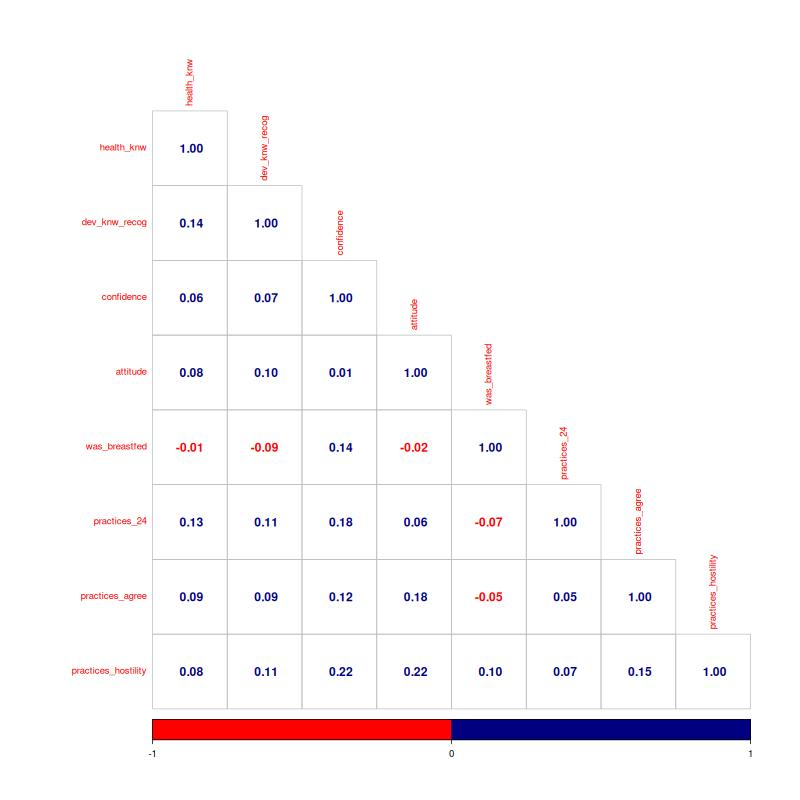
\includegraphics[scale=0.33]{descriptives/plots/correlations_constructs_Serbia_Baseline.jpg}
%     \caption{Construct Correlations - Serbia}
%     \label{fig:serbia correlations}
% \end{minipage}%
% \begin{minipage}{.5\textwidth}
%     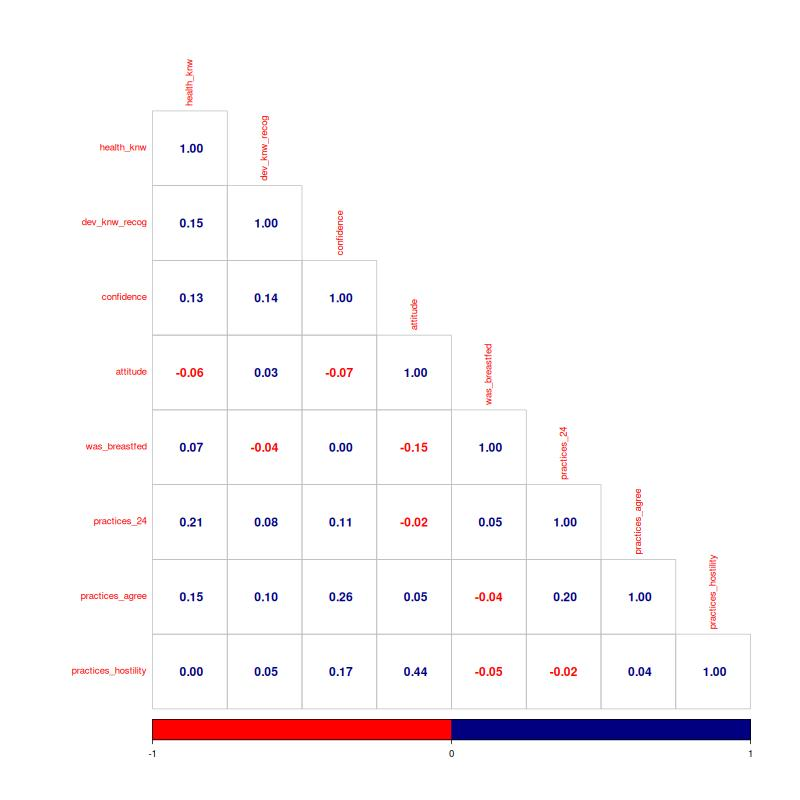
\includegraphics[scale=0.33]{descriptives/plots/correlations_constructs_Bulgaria_Baseline.jpg}
%     \caption{Construct Correlations - Bulgaria}
%     \label{fig:bulgaria correlations}
% \end{minipage}%
% \end{figure}

\addcontentsline{toc}{subsection}{Baseline Balance}
\subsection*{Baseline Balance}

To test for balance between our randomly assigned treatment and control groups, we run an omnibus test, following Hansen and Bowers (2008), to observe standardized differences at baseline and the associated omnibus p-value. Results are found in table \ref{tbl:Baseline Balance Pooled}.

The most notable variable is the practices\_24 and was\_breastfed, which differ a bit between the groups although they are still under 0.1 standard deviations in their diffrence. The omnibus test, with a p-value above 0.13, implies that the two groups are not different in a statistically significant manner.



% Table created by stargazer v.5.2.3 by Marek Hlavac, Social Policy Institute. E-mail: marek.hlavac at gmail.com
% Date and time: Sun, Jan 21, 2024 - 06:42:02 PM
\begin{table}[!htbp] \centering 
  \caption{Baseline Balance Pooled} 
  \label{tbl:Baseline Balance Pooled} 
\begin{tabular}{@{\extracolsep{5pt}} ccccc} 
\\[-1.8ex]\hline 
\hline \\[-1.8ex] 
 & control\_mean & treatment\_mean & standardized\_diff & z\_score \\ 
\hline \\[-1.8ex] 
health\_knw & $0.73$ & $0.71$ & $$-$0.06$ & $$-$1.20$ \\ 
dev\_knw\_recog & $0.86$ & $0.85$ & $$-$0.04$ & $$-$1.29$ \\ 
confidence & $3.33$ & $3.34$ & $0.01$ & $0.37$ \\ 
attitude & $3.14$ & $3.11$ & $$-$0.04$ & $$-$1.23$ \\ 
was\_breastfed & $0.35$ & $0.39$ & $0.08$ & $1.79$ \\ 
practices\_24 & $4.97$ & $4.87$ & $$-$0.07$ & $$-$2.46$ \\ 
practices\_agree & $3.20$ & $3.19$ & $$-$0.01$ & $$-$0.39$ \\ 
practices\_hostility & $3.03$ & $3.04$ & $0.004$ & $0.12$ \\ 
(health\_knw) & $0.42$ & $0.43$ & $0.02$ & $0.67$ \\ 
(was\_breastfed) & $0.42$ & $0.43$ & $0.02$ & $0.61$ \\ 
\hline \\[-1.8ex] 
\multicolumn{5}{l}{Overall P-Value: 0.134132865981628} \\ 
\end{tabular} 
\end{table} 

% 
% Table created by stargazer v.5.2.3 by Marek Hlavac, Social Policy Institute. E-mail: marek.hlavac at gmail.com
% Date and time: Mon, Mar 11, 2024 - 09:43:35 PM
\begin{table}[!htbp] \centering 
  \caption{Baseline Balance Serbia} 
  \label{tbl:Baseline Balance Serbia} 
\begin{tabular}{@{\extracolsep{5pt}} ccccc} 
\\[-1.8ex]\hline 
\hline \\[-1.8ex] 
 & control\_mean & treatment\_mean & standardized\_diff & z\_score \\ 
\hline \\[-1.8ex] 
health\_knw & $0.78$ & $0.75$ & $$-$0.07$ & $$-$1.16$ \\ 
dev\_knw\_recog & $0.87$ & $0.88$ & $0.02$ & $0.62$ \\ 
confidence & $3.38$ & $3.39$ & $0.02$ & $0.57$ \\ 
attitude & $3.08$ & $3.08$ & $$-$0.01$ & $$-$0.17$ \\ 
was\_breastfed & $0.39$ & $0.42$ & $0.07$ & $1.19$ \\ 
practices\_24 & $5.09$ & $4.99$ & $$-$0.09$ & $$-$2.39$ \\ 
practices\_agree & $2.95$ & $2.94$ & $$-$0.02$ & $$-$0.42$ \\ 
practices\_hostility & $3.07$ & $3.05$ & $$-$0.03$ & $$-$0.75$ \\ 
(health\_knw) & $0.40$ & $0.41$ & $0.02$ & $0.63$ \\ 
\hline \\[-1.8ex] 
\multicolumn{5}{l}{Overall P-Value: 0.307} \\ 
\end{tabular} 
\end{table} 

% 
% Table created by stargazer v.5.2.3 by Marek Hlavac, Social Policy Institute. E-mail: marek.hlavac at gmail.com
% Date and time: Tue, Mar 12, 2024 - 11:42:36 PM
\begin{table}[!htbp] \centering 
  \caption{Baseline Balance Bulgaria} 
  \label{tbl:Baseline Balance Bulgaria} 
\begin{tabular}{@{\extracolsep{5pt}} ccccc} 
\\[-1.8ex]\hline 
\hline \\[-1.8ex] 
 & control\_mean & treatment\_mean & standardized\_diff & z\_score \\ 
\hline \\[-1.8ex] 
health\_knw & $0.67$ & $0.65$ & $$-$0.04$ & $$-$0.56$ \\ 
dev\_knw\_recog & $0.85$ & $0.81$ & $$-$0.13$ & $$-$2.71$ \\ 
confidence & $3.27$ & $3.26$ & $$-$0.01$ & $$-$0.21$ \\ 
attitude & $3.23$ & $3.16$ & $$-$0.08$ & $$-$1.57$ \\ 
was\_breastfed & $0.31$ & $0.35$ & $0.10$ & $1.37$ \\ 
practices\_24 & $4.78$ & $4.71$ & $$-$0.06$ & $$-$1.15$ \\ 
practices\_agree & $3.59$ & $3.59$ & $0.02$ & $0.37$ \\ 
practices\_hostility & $2.97$ & $3.00$ & $0.05$ & $1.06$ \\ 
(health\_knw) & $0.45$ & $0.46$ & $0.02$ & $0.40$ \\ 
(was\_breastfed) & $0.45$ & $0.46$ & $0.01$ & $0.30$ \\ 
\hline \\[-1.8ex] 
\multicolumn{5}{l}{Overall P-Value: 0.034} \\ 
\end{tabular} 
\end{table} 


% \clearpage

% \section*{Baseline Construct Distributions}

% 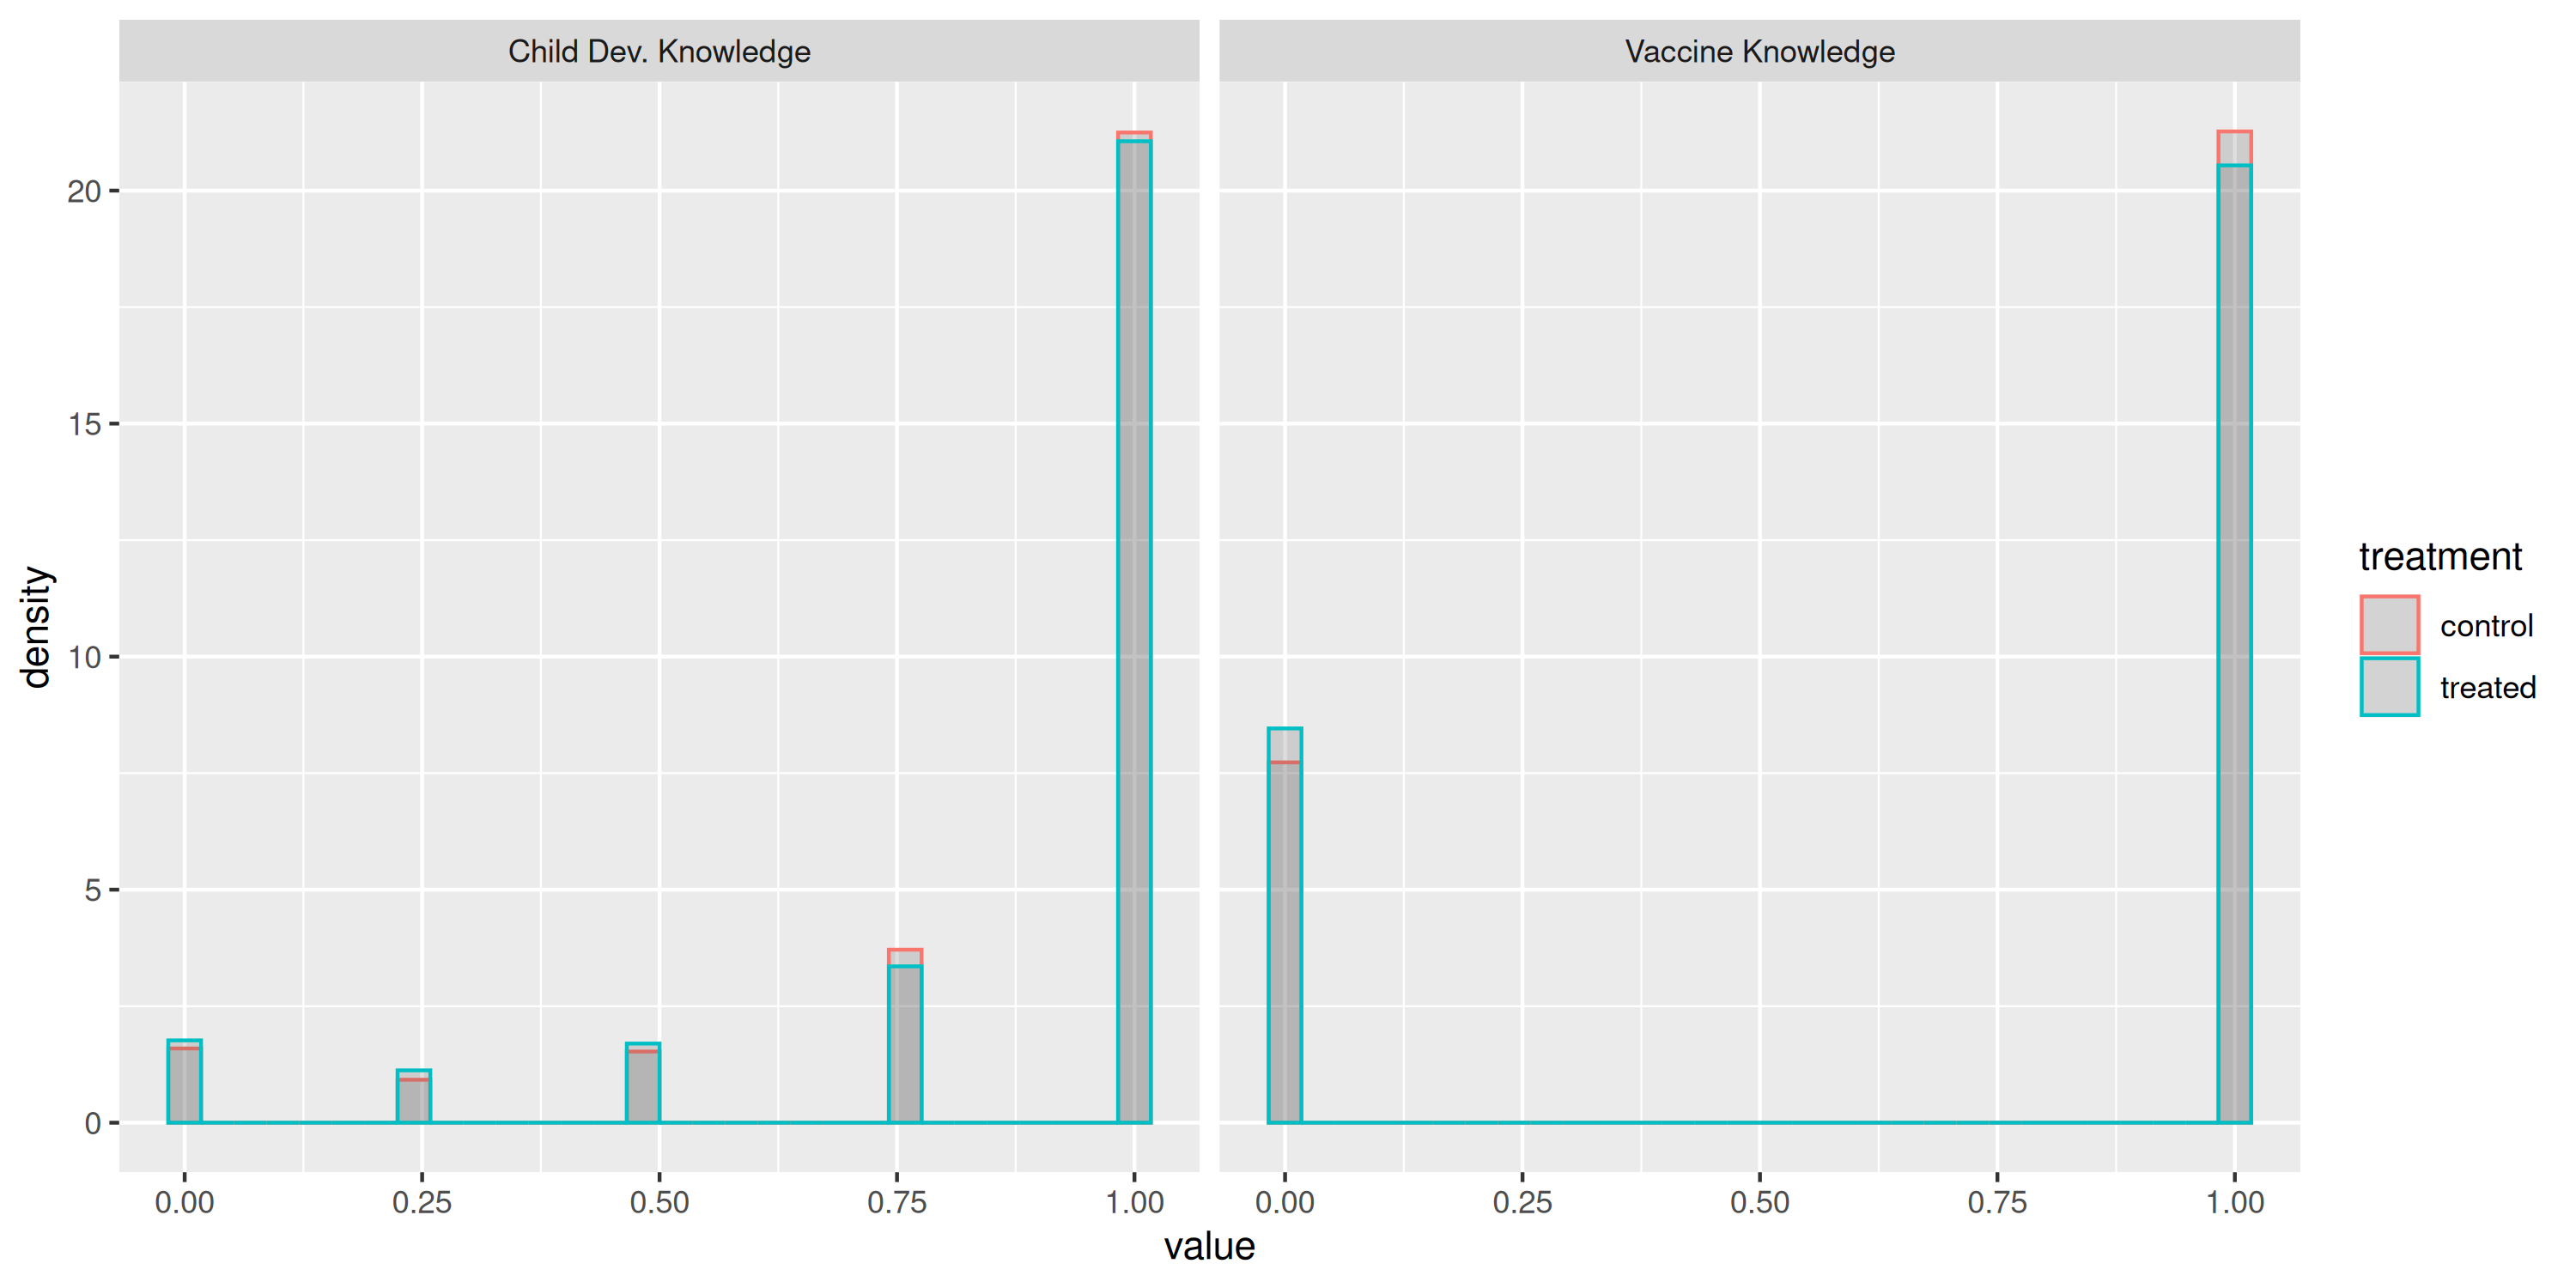
\includegraphics[width=\textwidth]{plots/Original Data - Knowledge and Awareness.png}
% 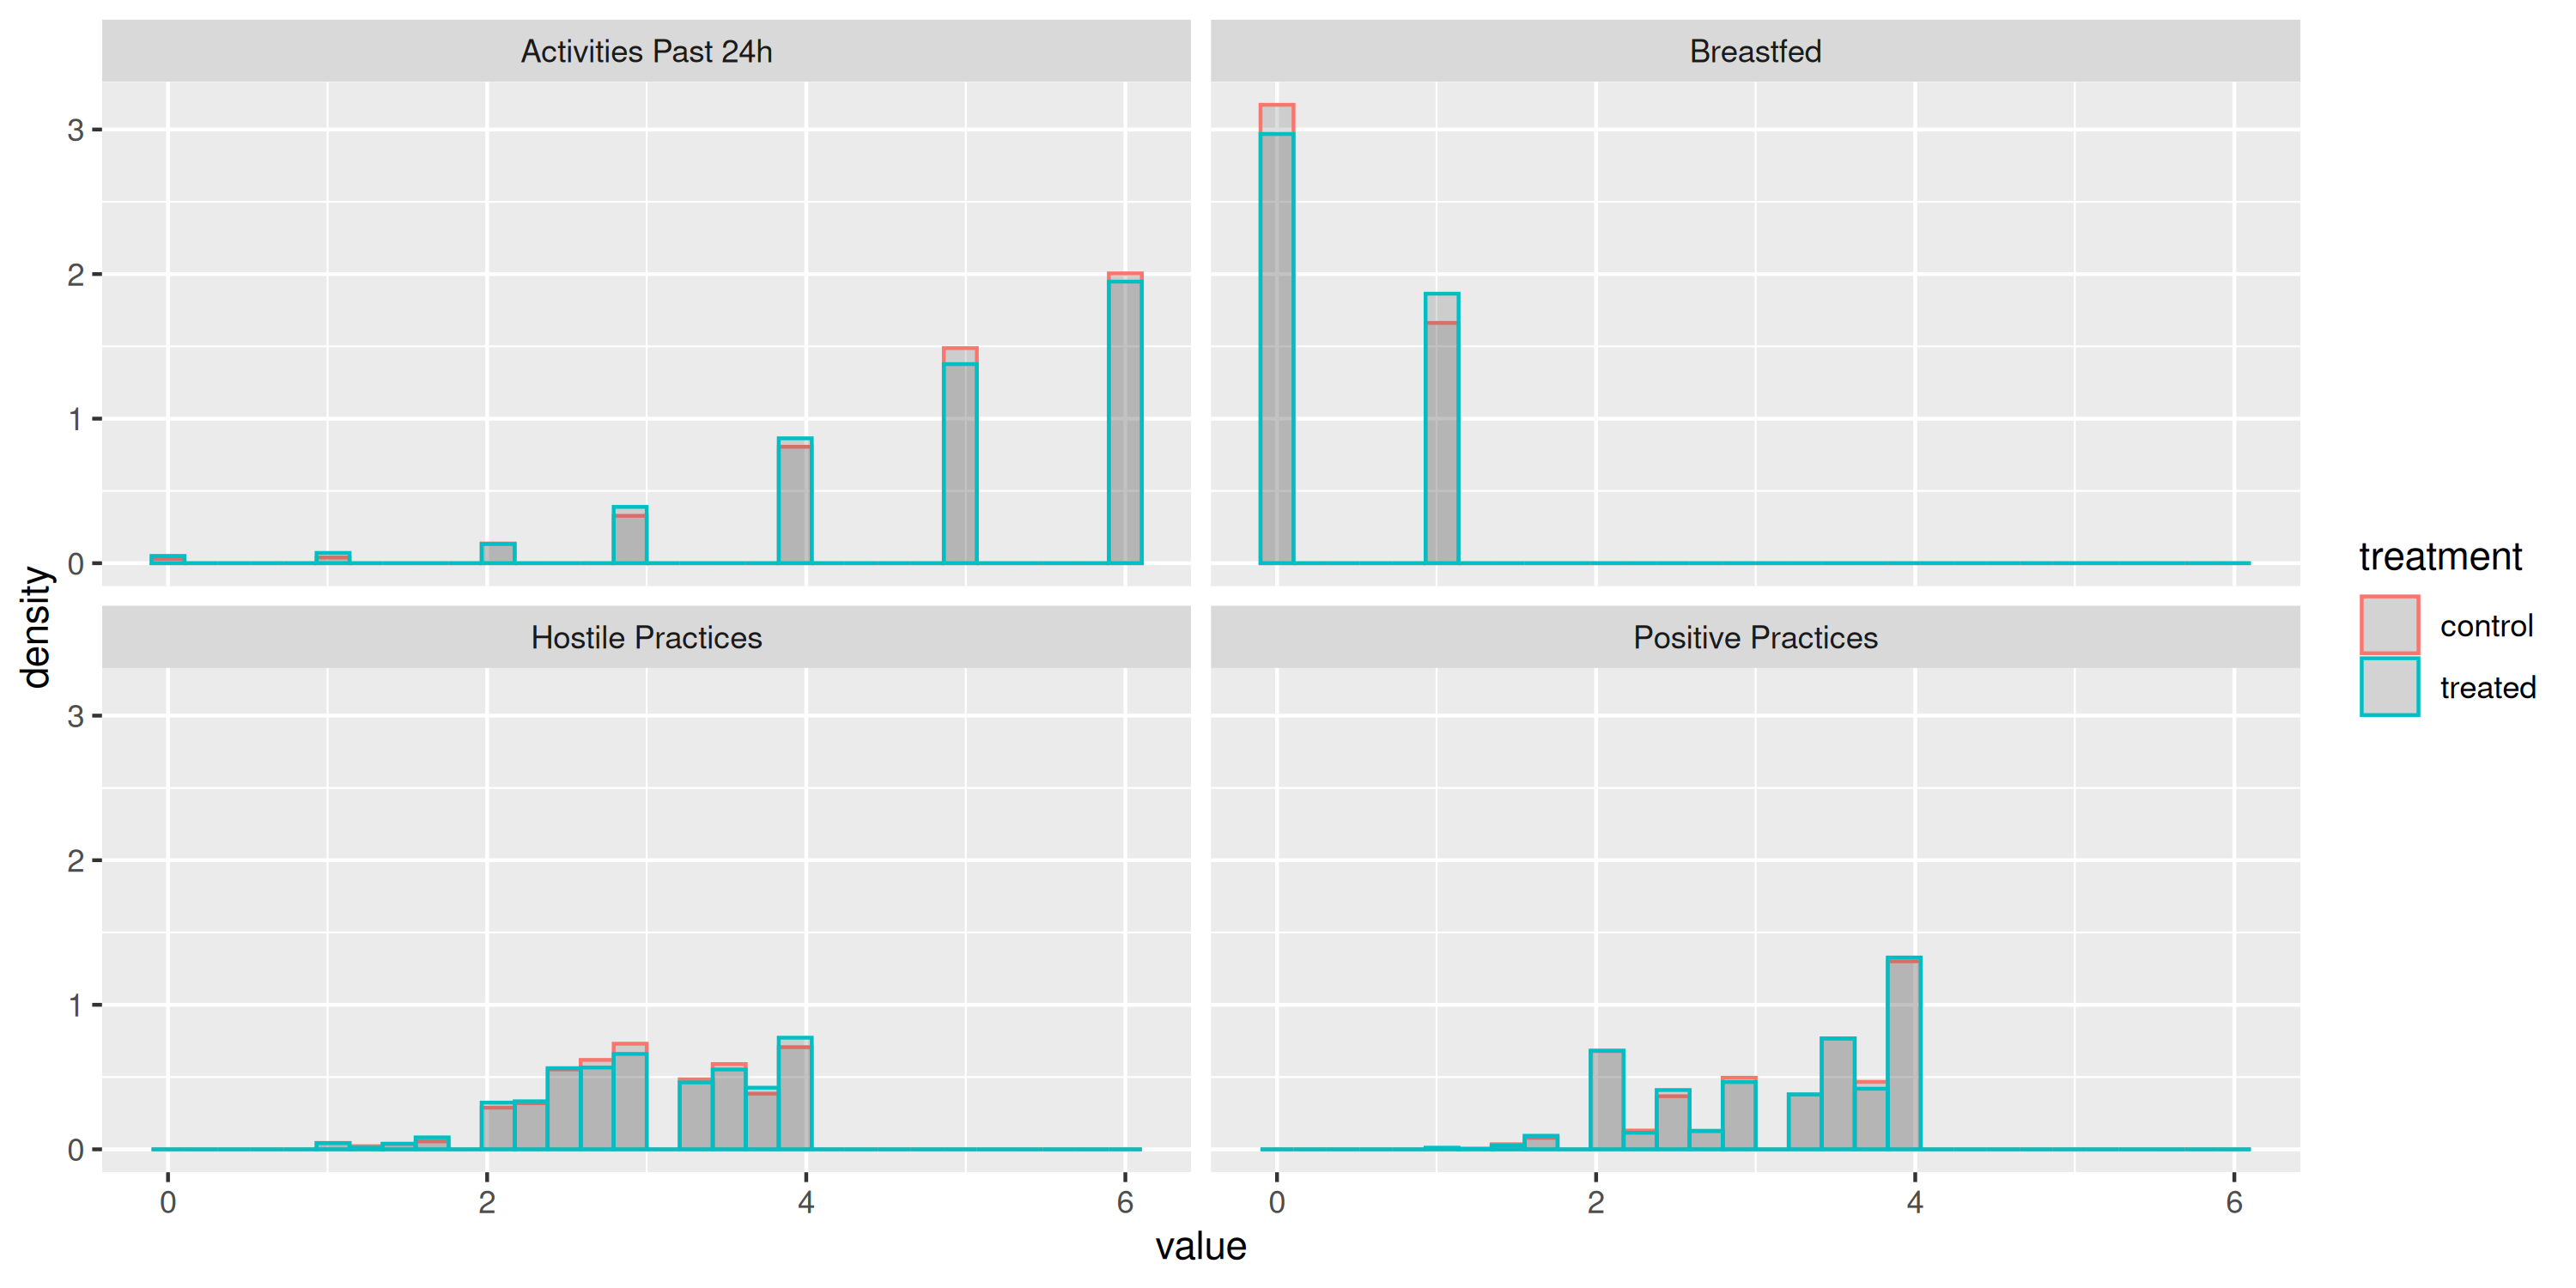
\includegraphics[width=\textwidth]{plots/Original Data - Practices.png}
% 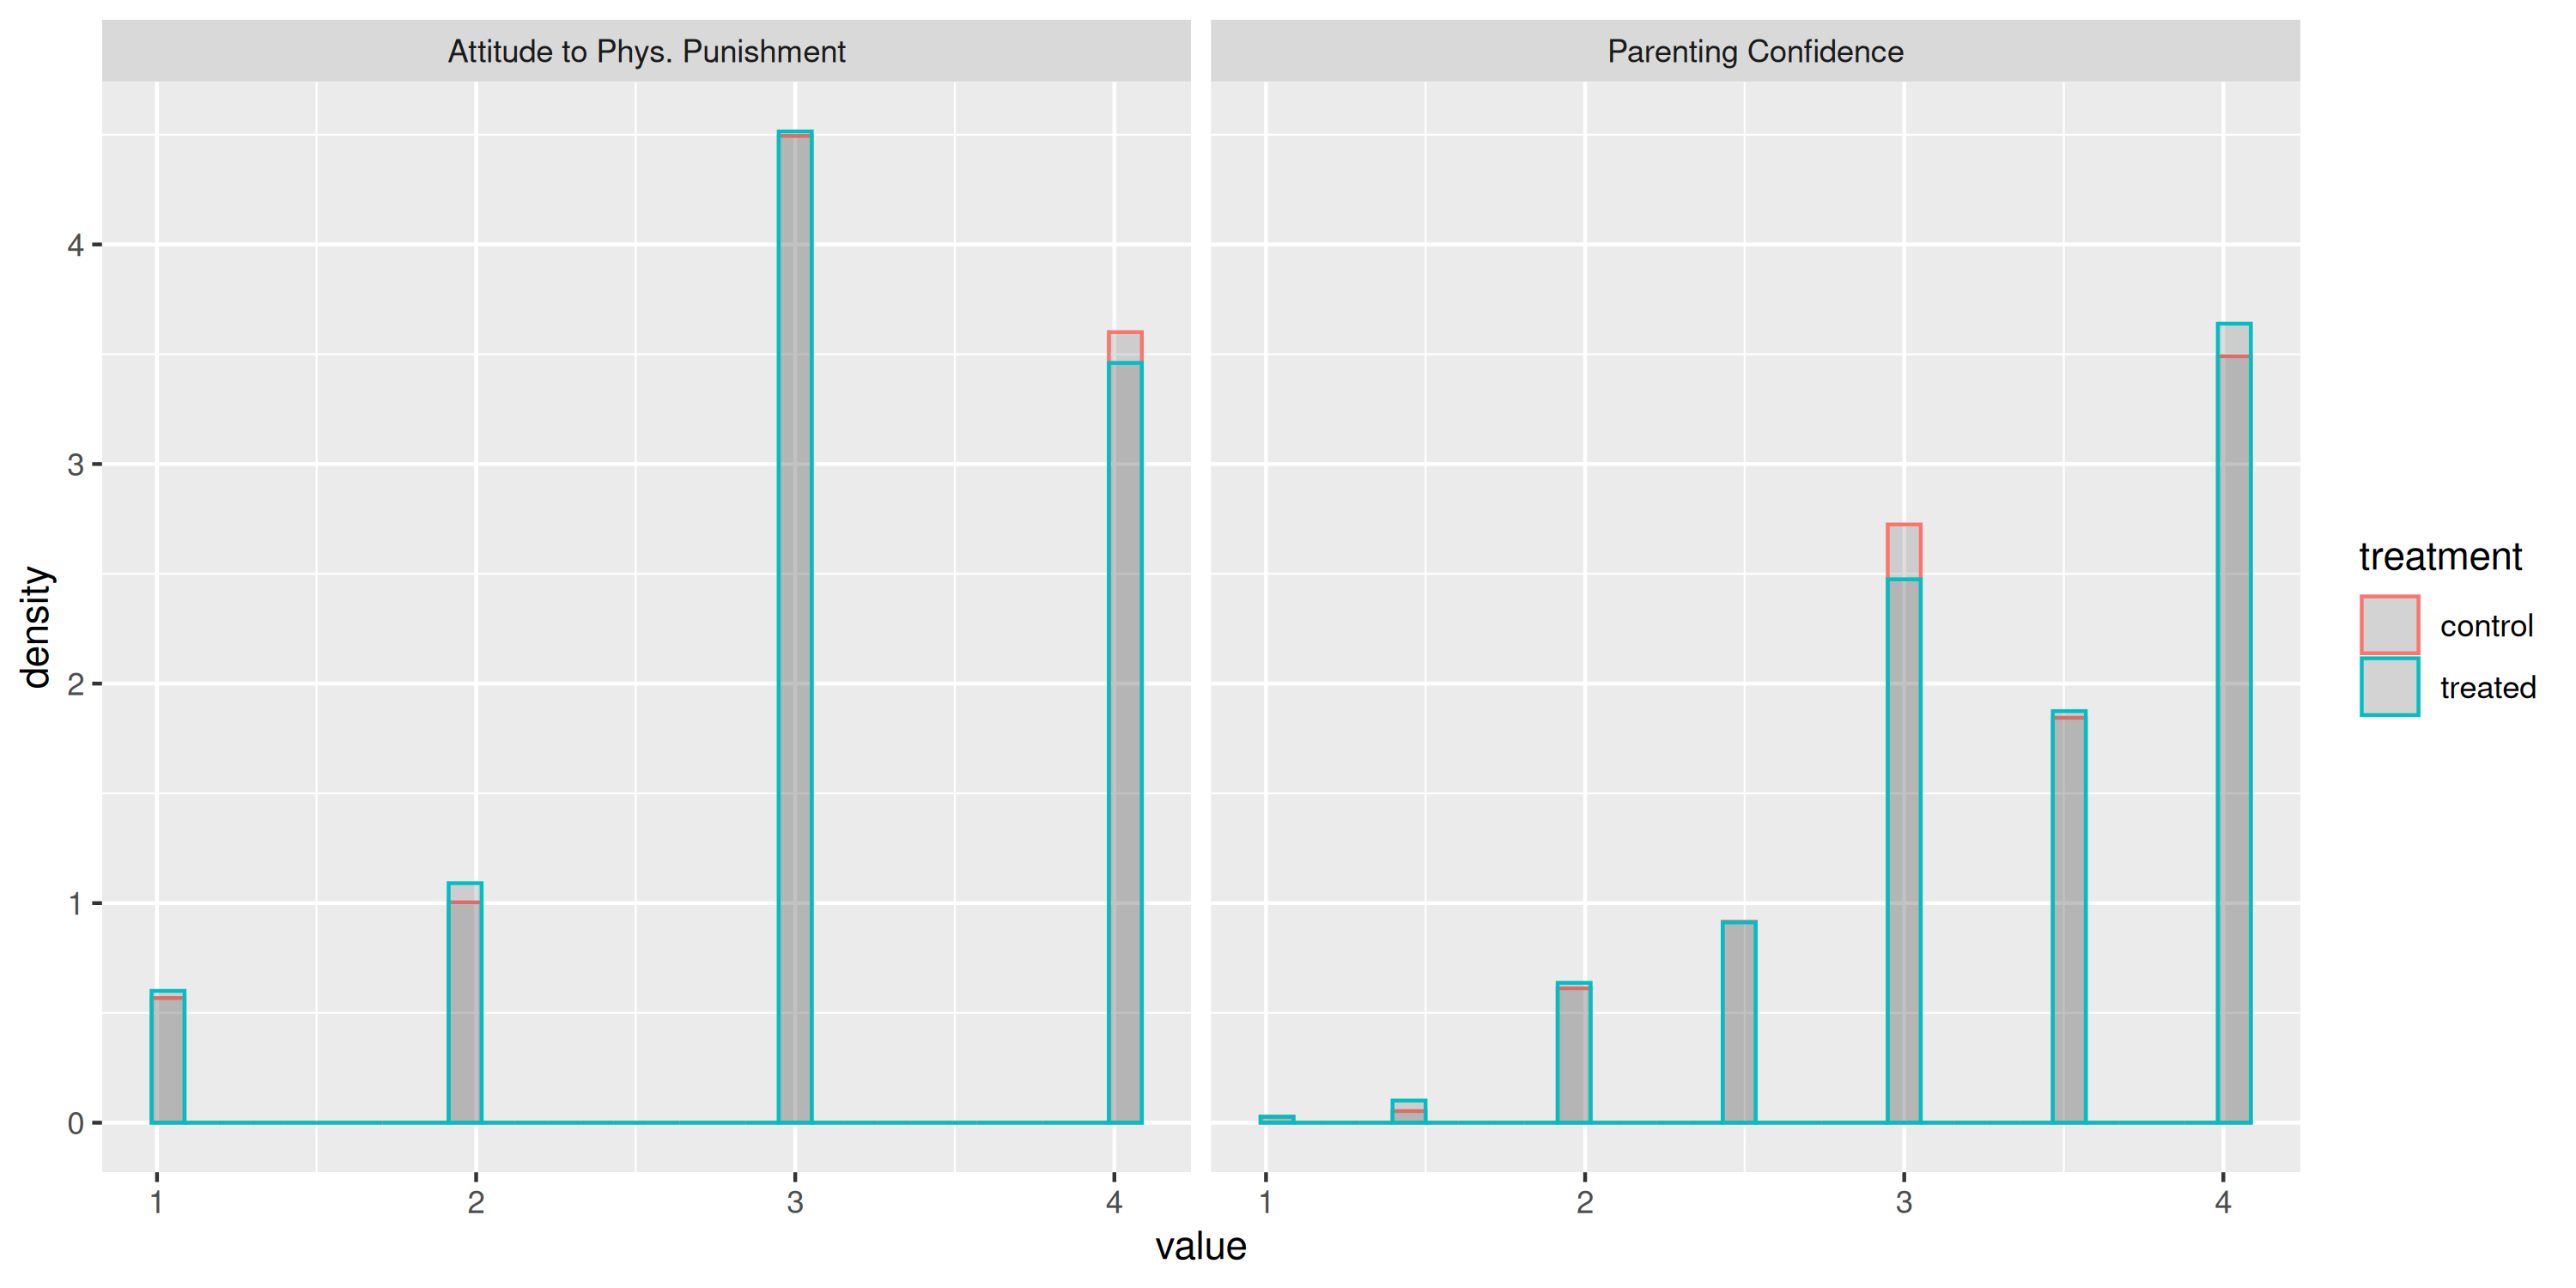
\includegraphics[width=\textwidth]{plots/Original Data - Confidence and Attitudes.png}


% \clearpage

% \section*{Transformed Construct Distributions}
% 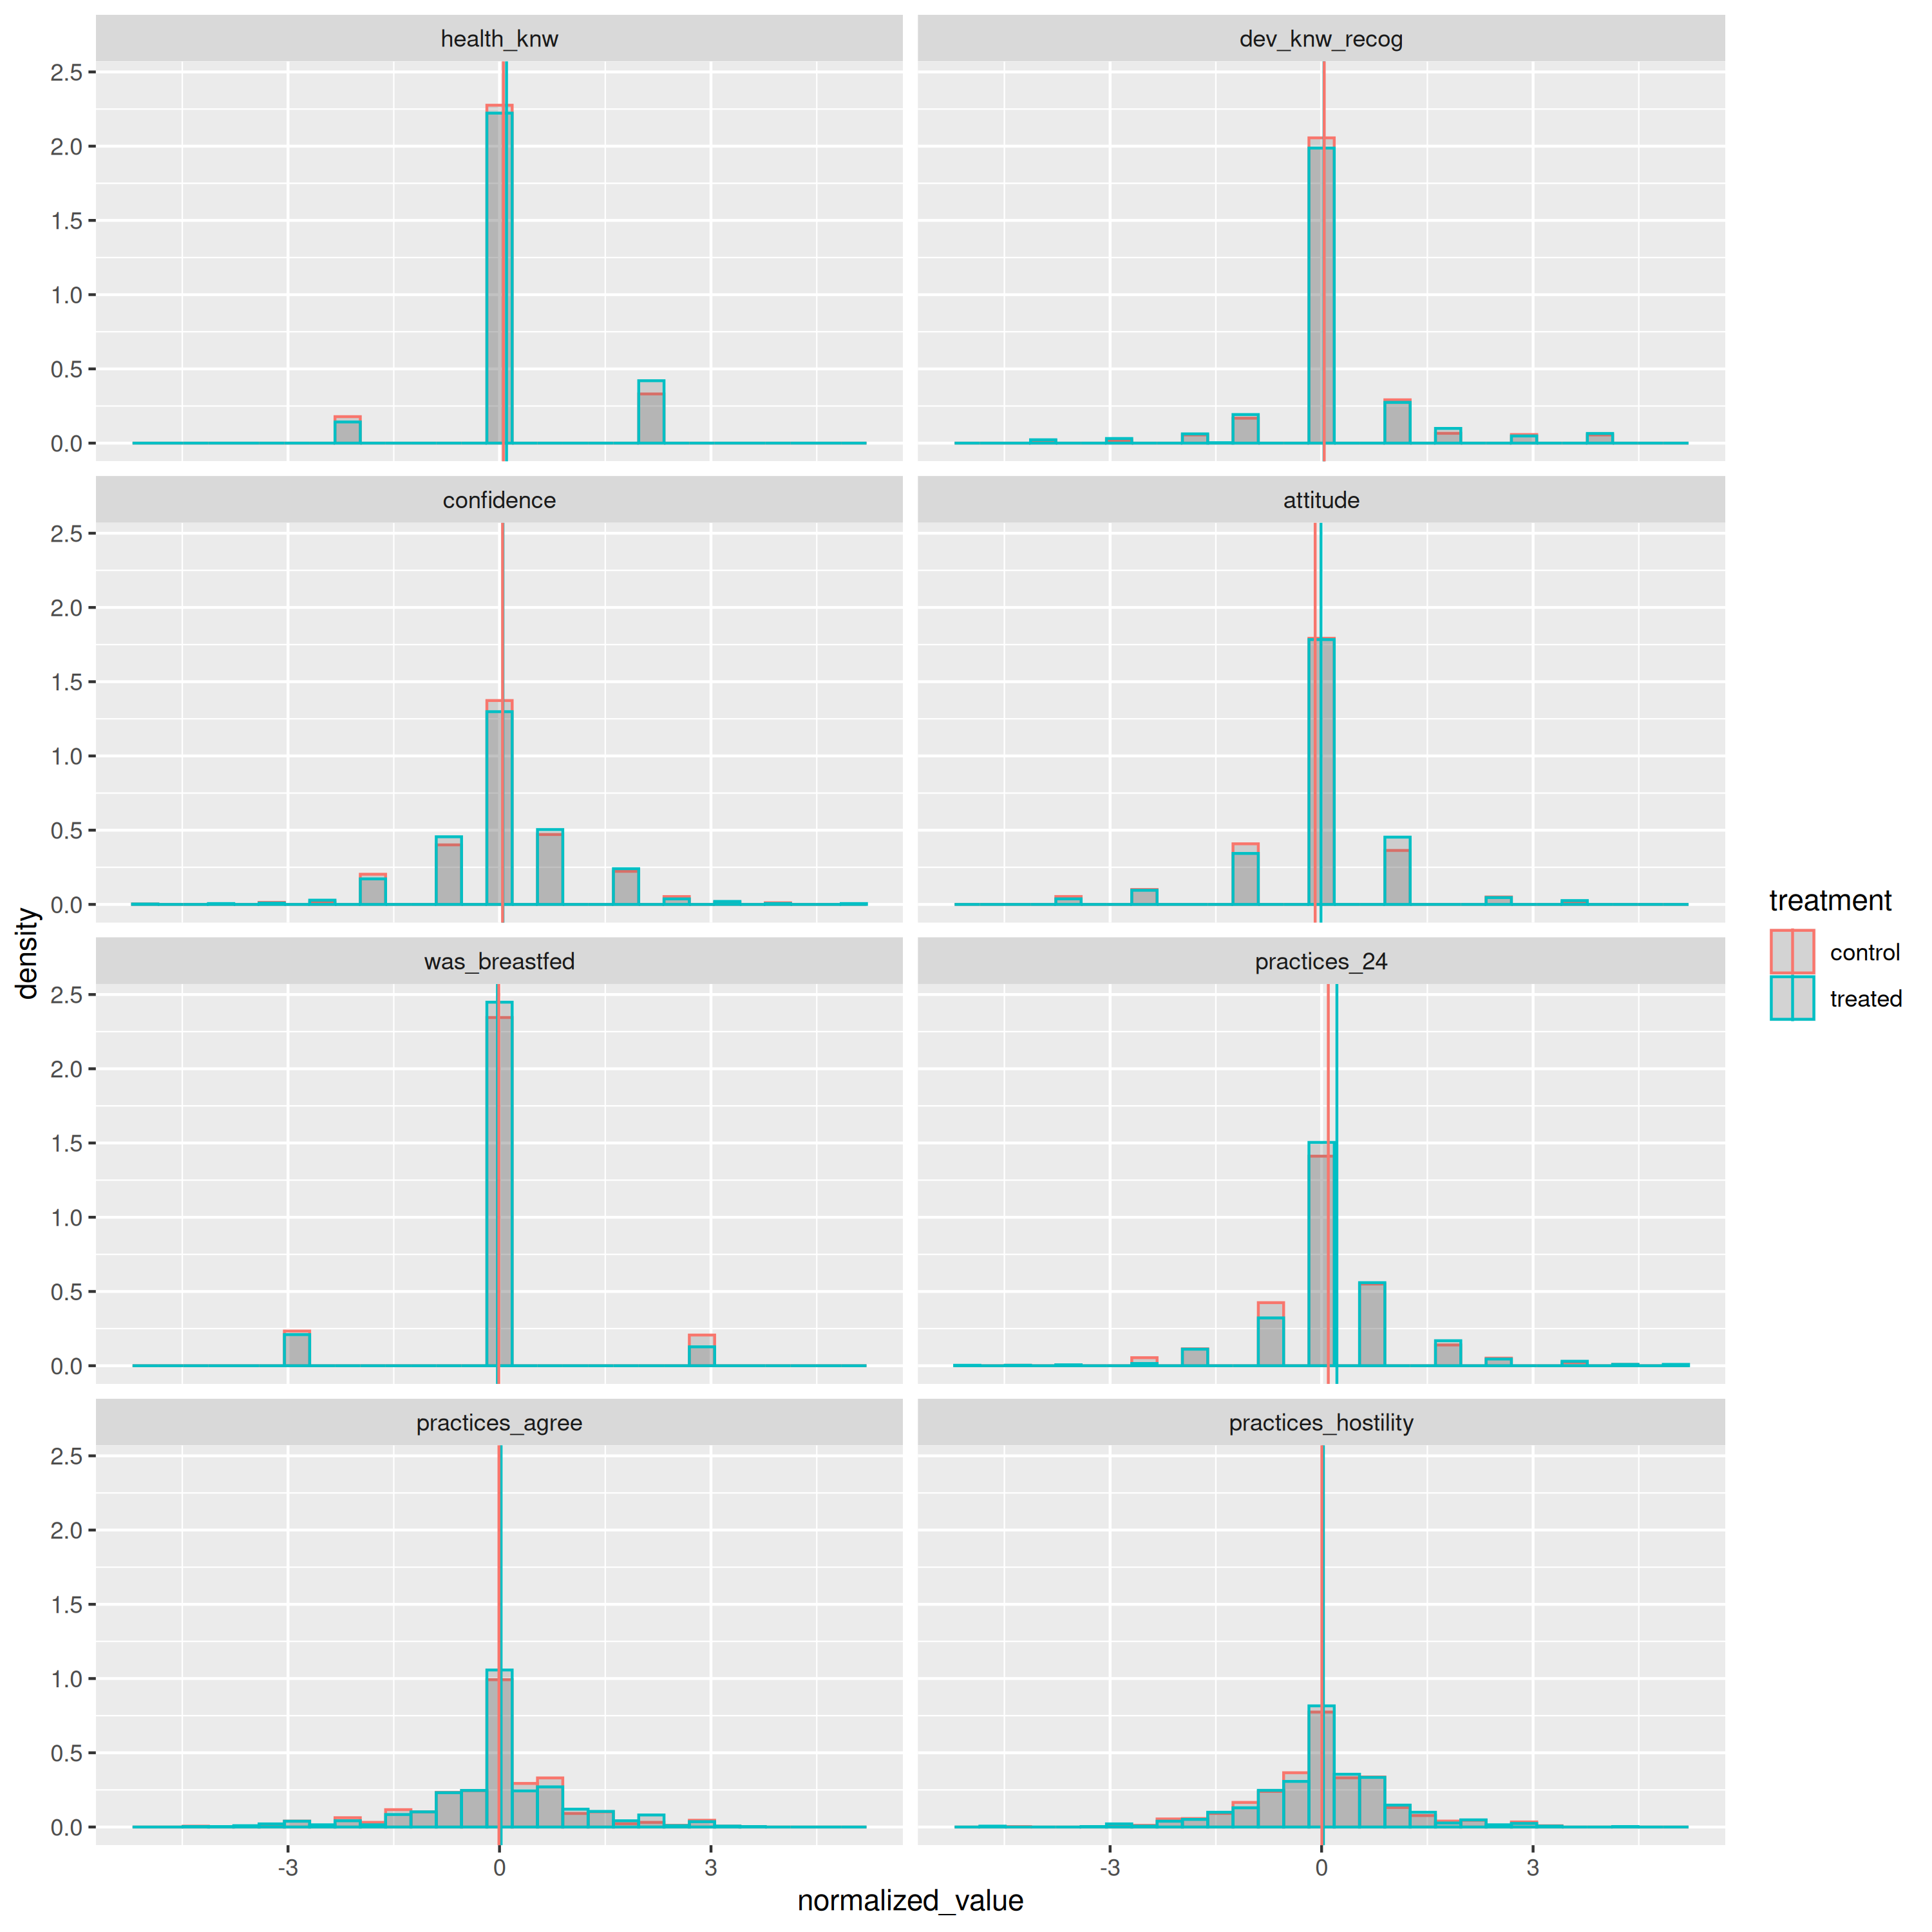
\includegraphics[width=\textwidth]{plots/Transformed Data.png}


% \clearpage


% \section*{Pre Post Data}
% 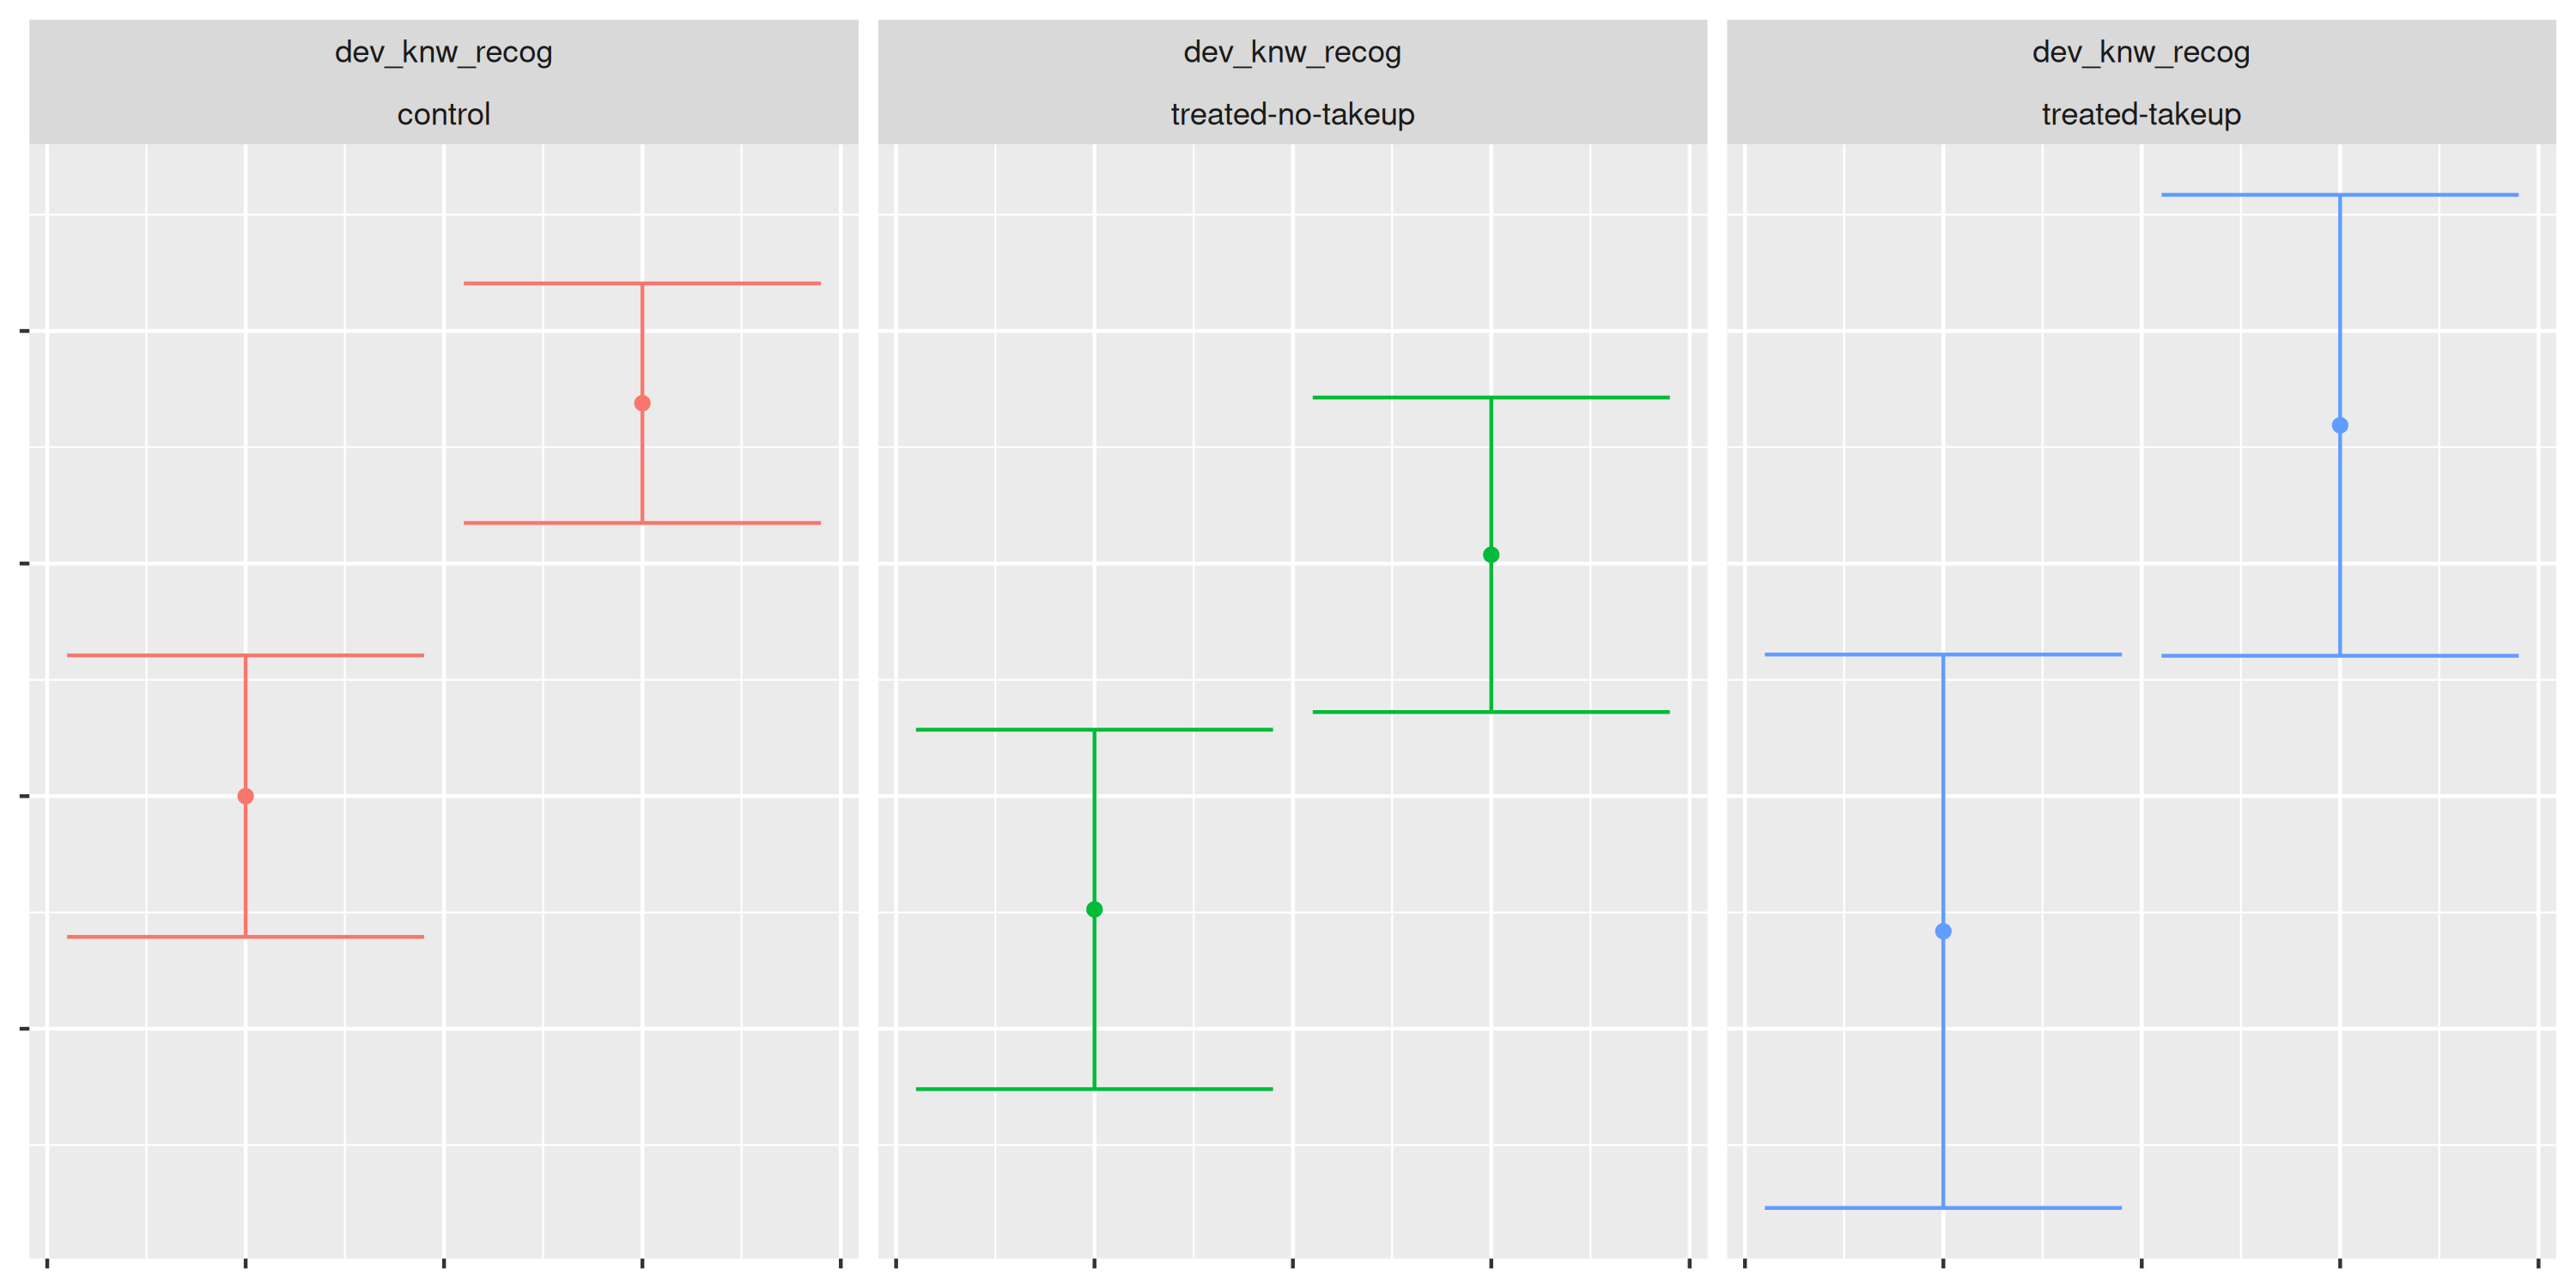
\includegraphics[width=\textwidth]{plots/pre_post/health_knw.png}
% 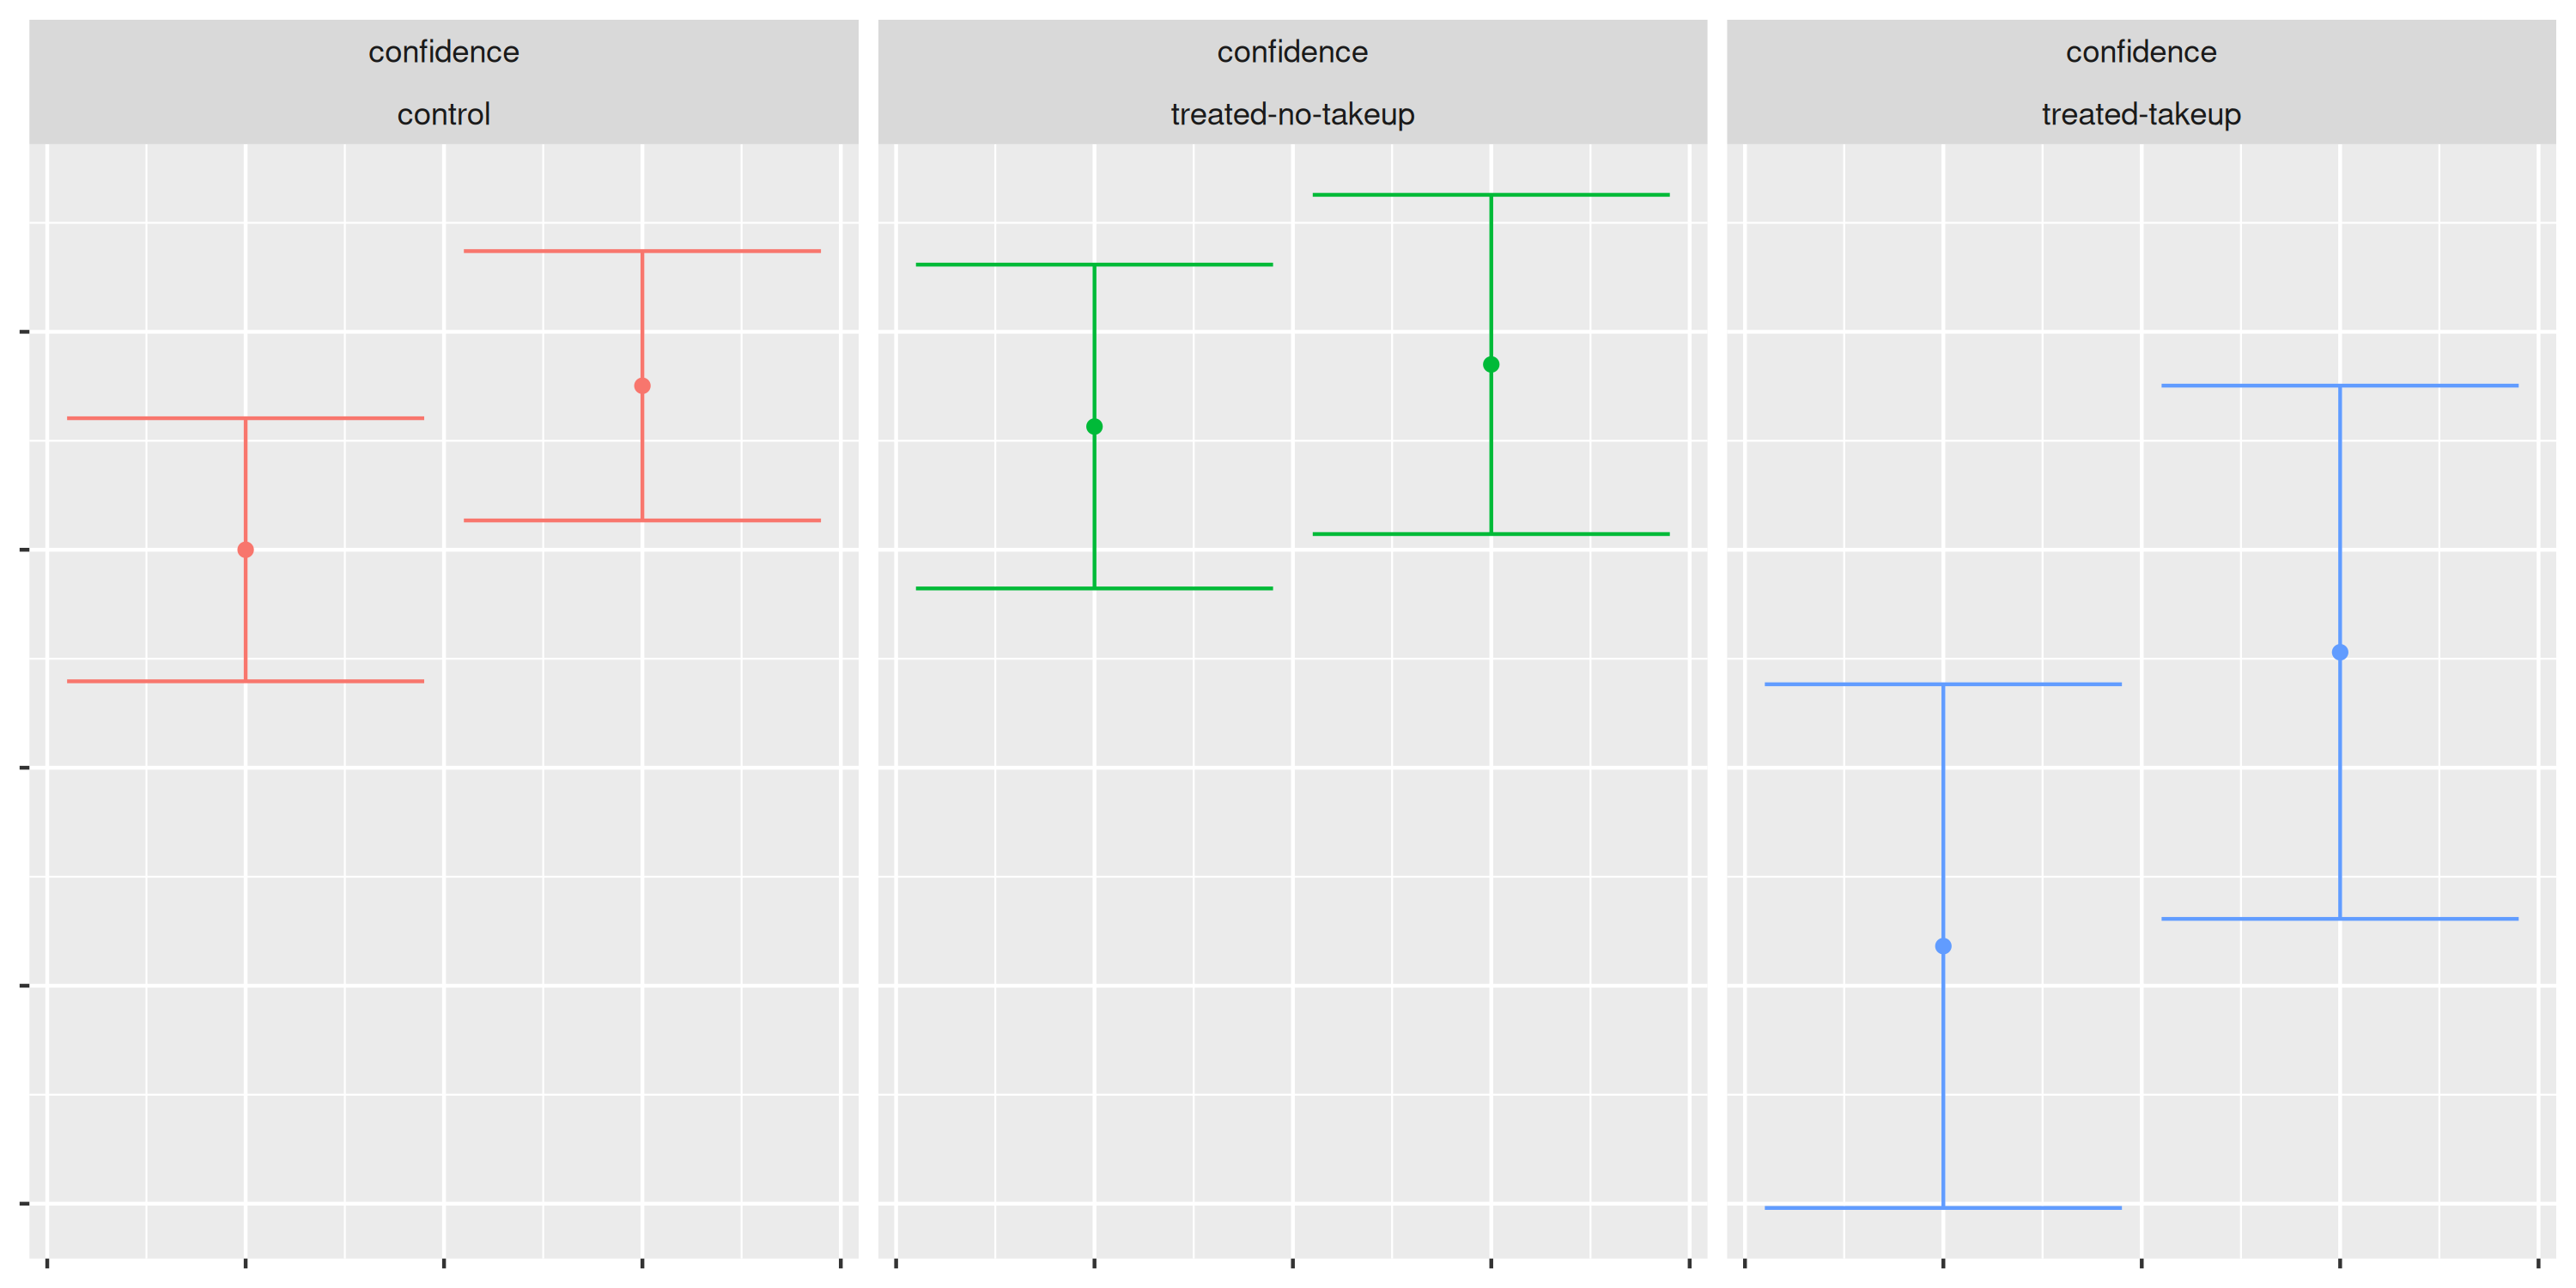
\includegraphics[width=\textwidth]{plots/pre_post/confidence.png}
% 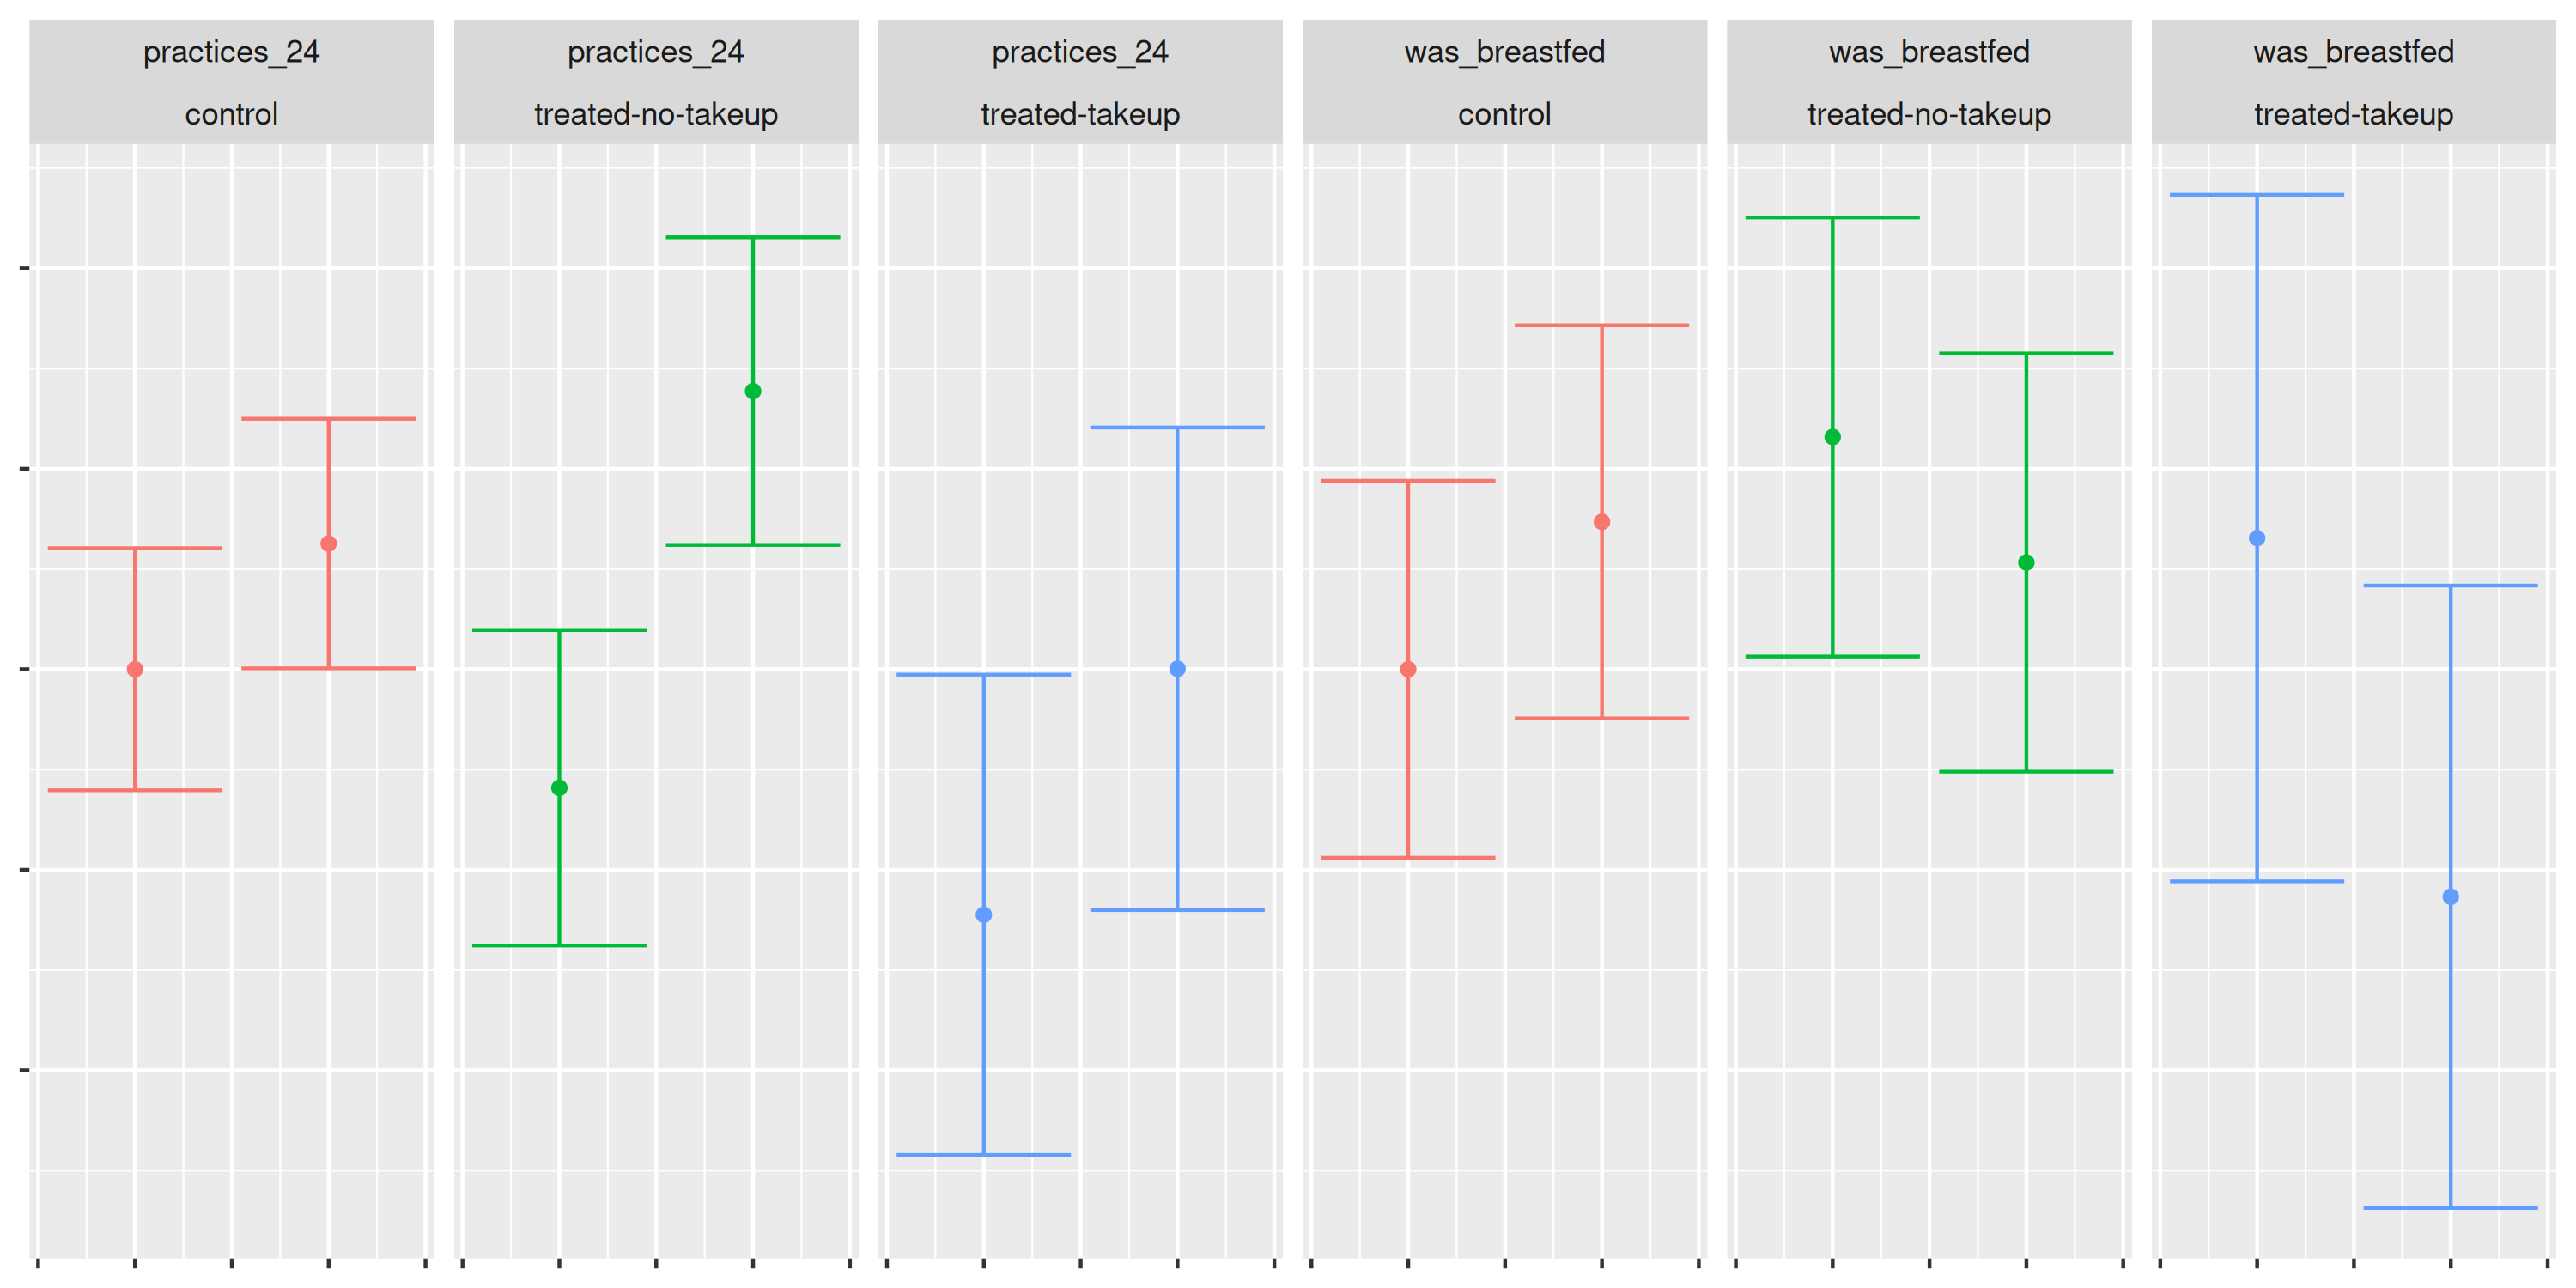
\includegraphics[width=\textwidth]{plots/pre_post/was_breastfed.png}
% 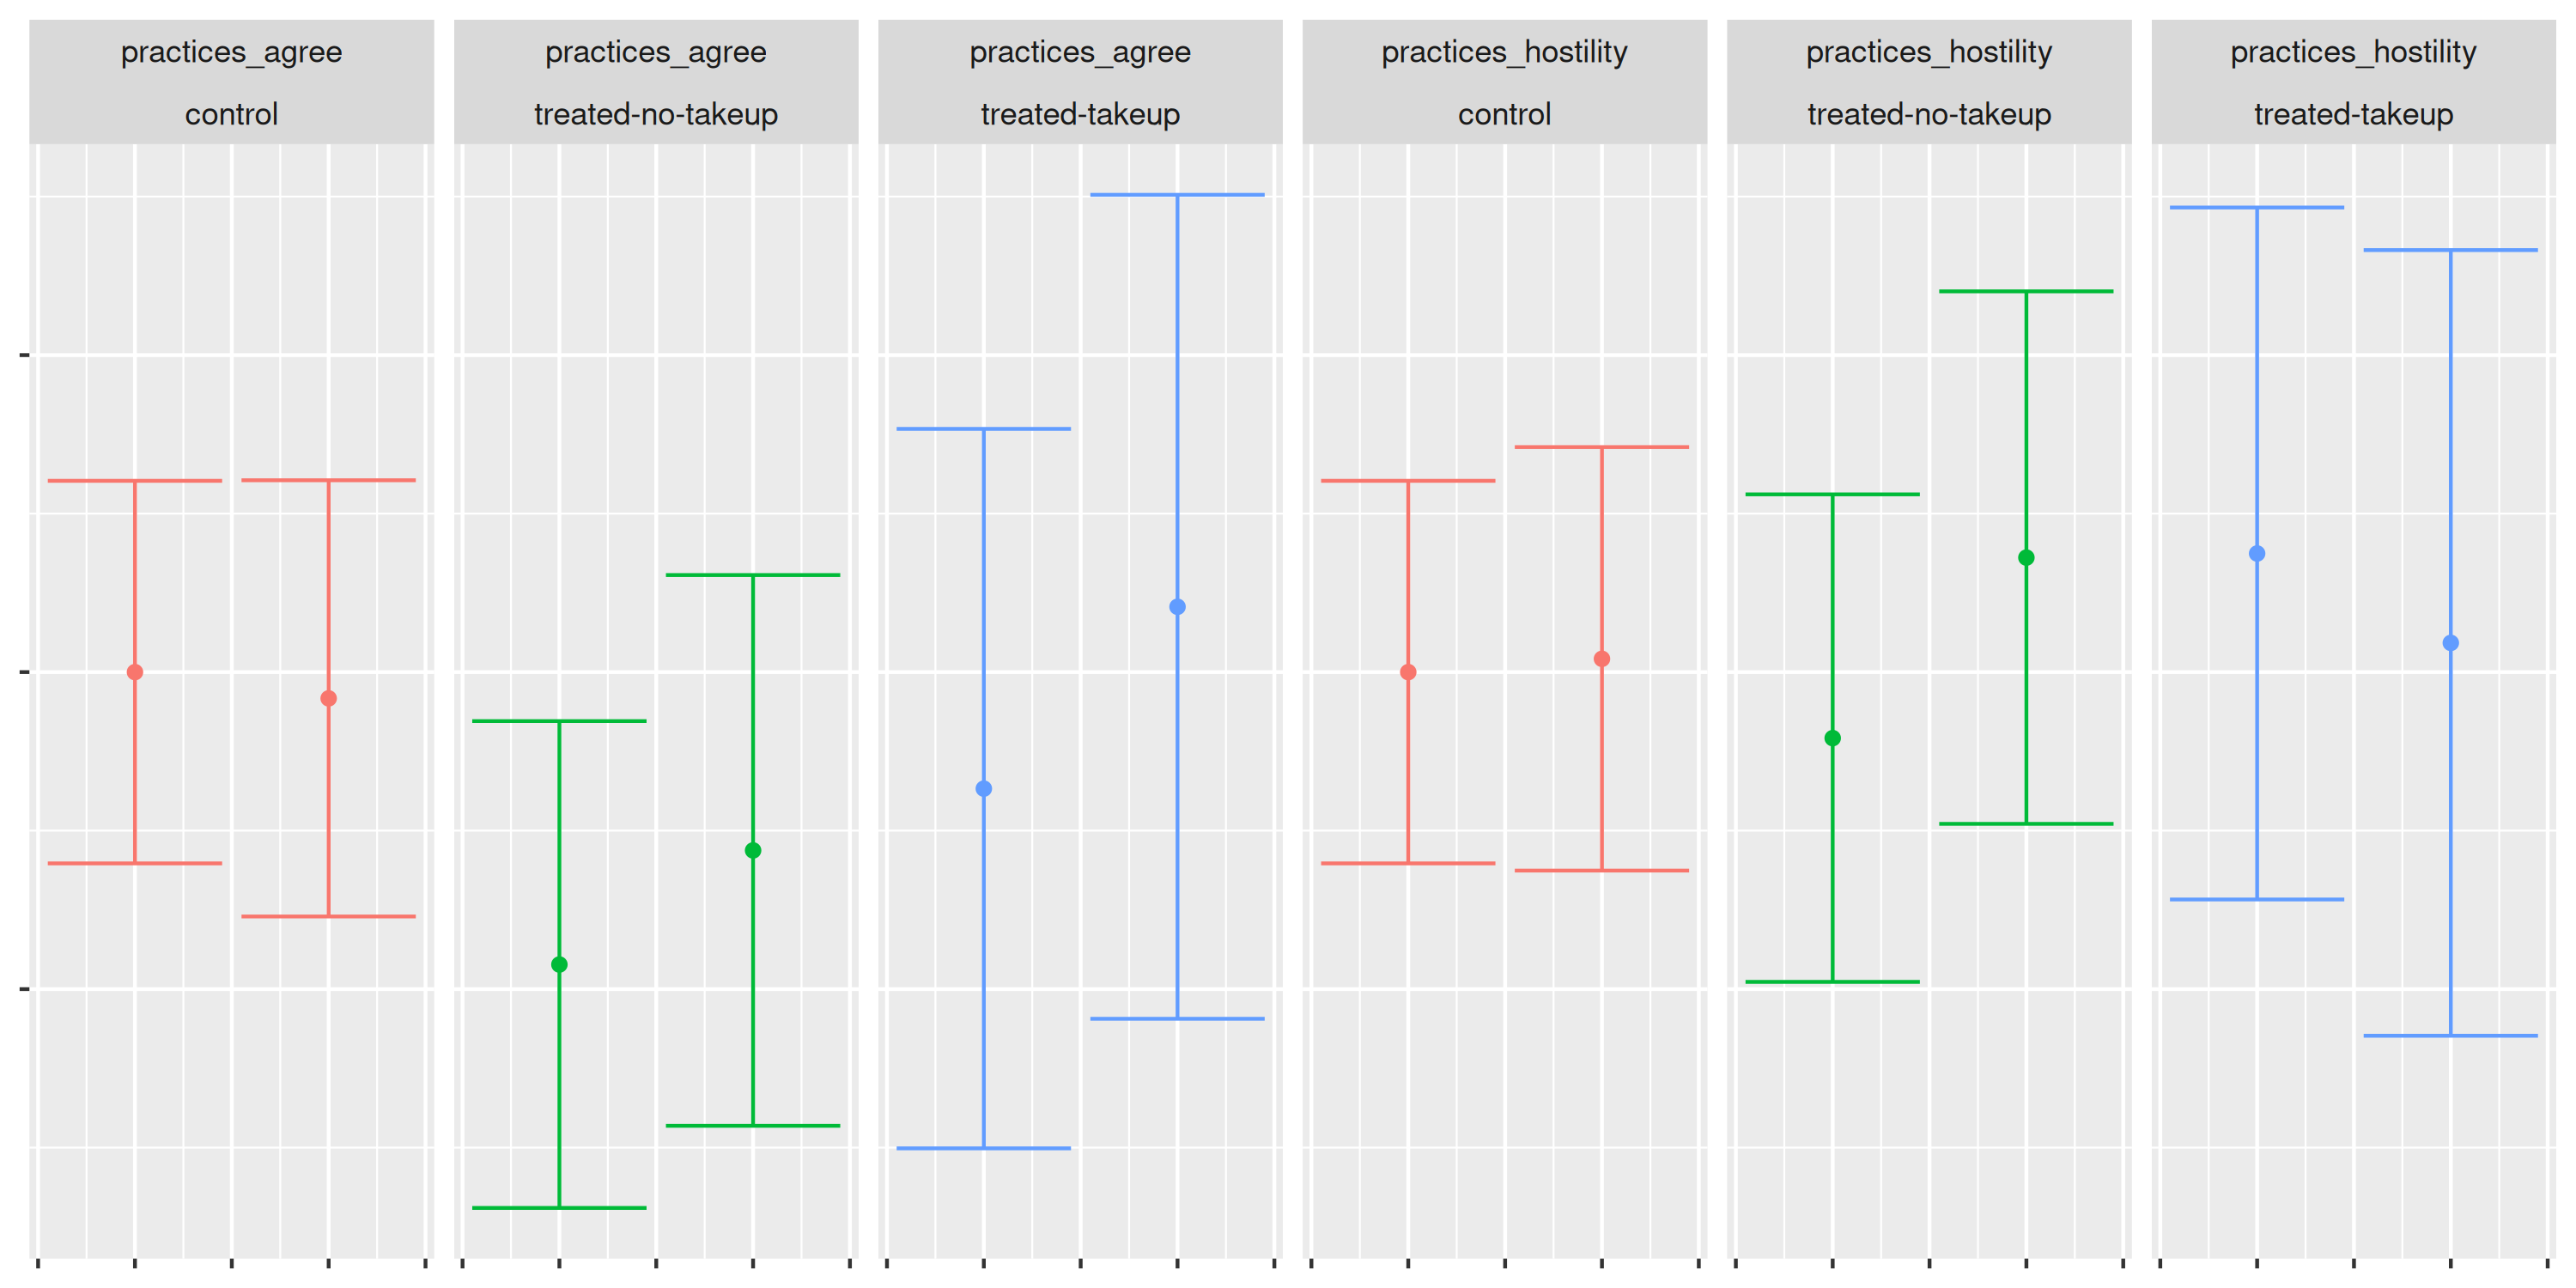
\includegraphics[width=\textwidth]{plots/pre_post/practices_agree.png}


% \clearpage

% \section*{Bebbo Usage in Control}

% Checking for contamination or baseline usage in the control group, we ask control group users, at the end of the final follow up survey, if they have ever heard of Bebbo or used Bebbo.

% 
% Table created by stargazer v.5.2.3 by Marek Hlavac, Social Policy Institute. E-mail: marek.hlavac at gmail.com
% Date and time: Thu, Nov 23, 2023 - 10:08:23 AM
\begin{table}[!htbp] \centering 
  \caption{Bebbo Usage in Control Group} 
  \label{tbl:Bebbo Usage in Control Group} 
\begin{tabular}{@{\extracolsep{5pt}} ccccc} 
\\[-1.8ex]\hline 
\hline \\[-1.8ex] 
dataset & name & value & count & freq \\ 
\hline \\[-1.8ex] 
Serbia & control\_bebbo\_knowledge & No &  89 & 0.4472362 \\ 
Serbia & control\_bebbo\_knowledge & Yes & 110 & 0.5527638 \\ 
Serbia & control\_bebbo\_usage & No & 153 & 0.7688442 \\ 
Serbia & control\_bebbo\_usage & Yes &  46 & 0.2311558 \\ 
Pooled & control\_bebbo\_knowledge & No & 152 & 0.3362832 \\ 
Pooled & control\_bebbo\_knowledge & Yes & 300 & 0.6637168 \\ 
Pooled & control\_bebbo\_usage & No & 269 & 0.5951327 \\ 
Pooled & control\_bebbo\_usage & Yes & 183 & 0.4048673 \\ 
\hline \\[-1.8ex] 
\end{tabular} 
\end{table} 


% \clearpage


% \section*{Power}

% 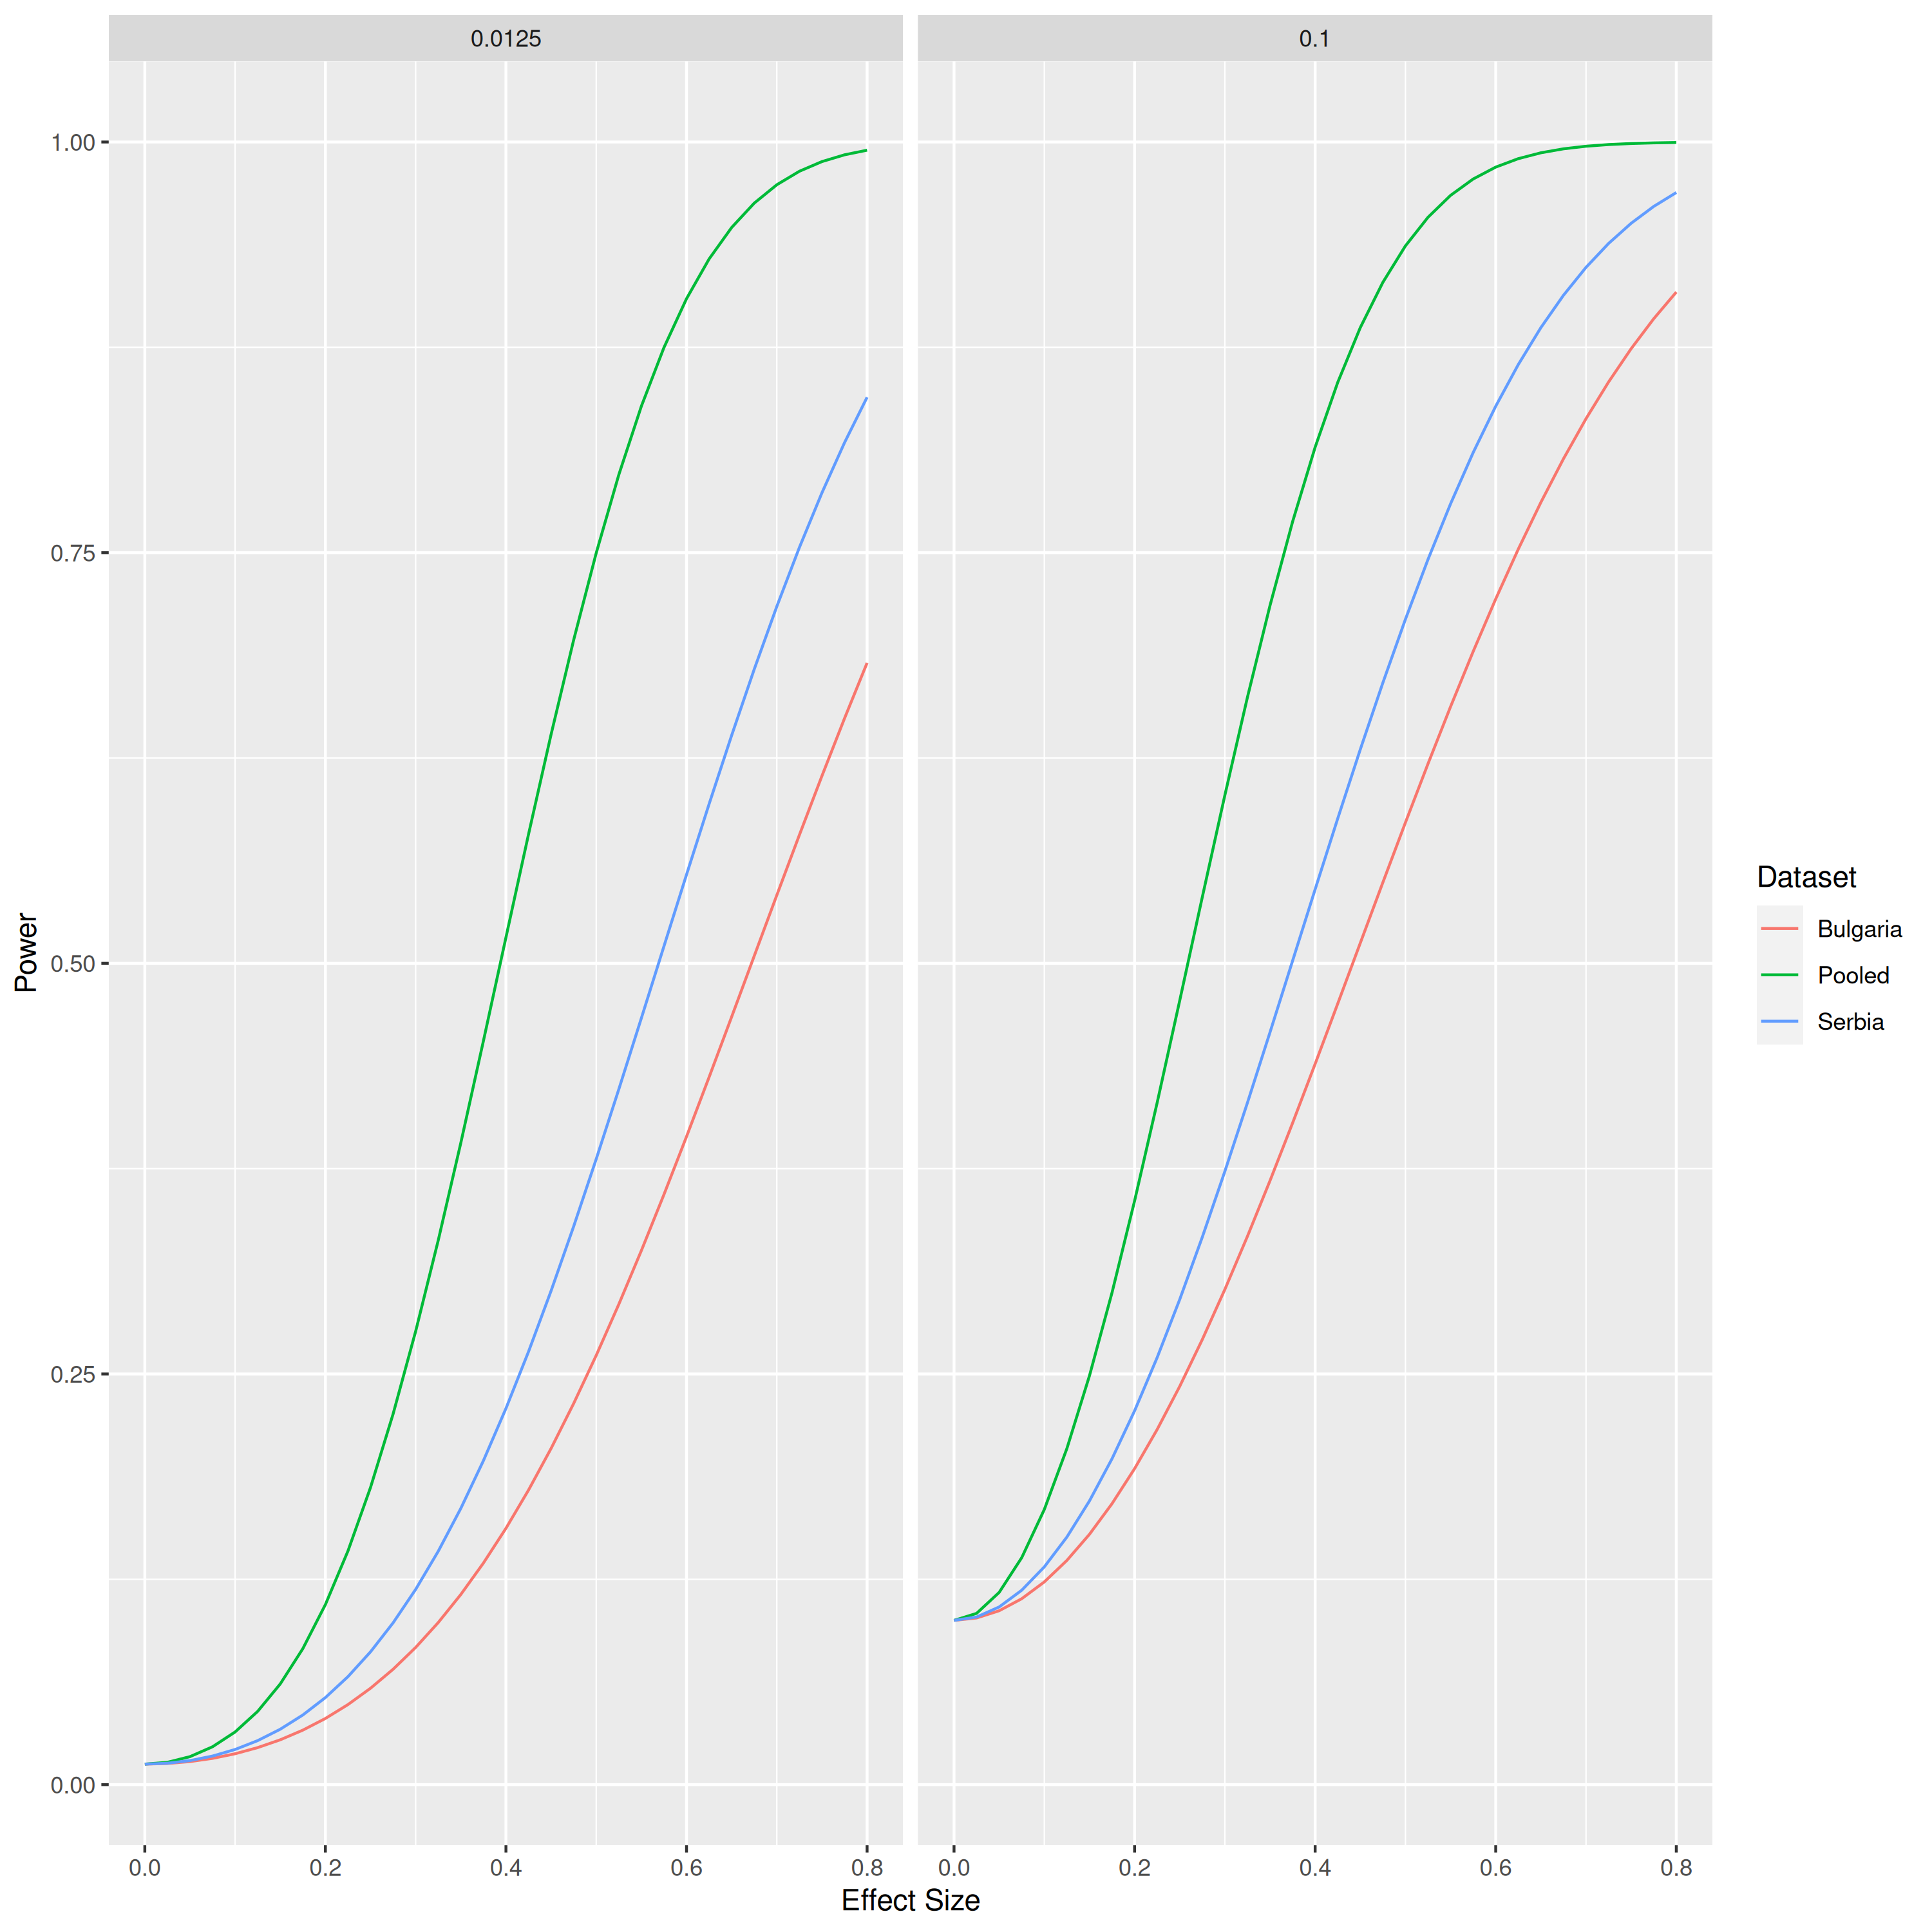
\includegraphics[width=\textwidth]{plots/Power Calculations.png}

% \clearpage

% \section*{Regression}

% We run the following regression model to measure the intent-to-treat effect (ITT) of assignment to the treatment arm on the outcome construct ($c$) of interest for individual $i$:

% $$
% y_{i} = \alpha + \beta T_{i} + \gamma_1X_{i} + \gamma_2Z_i + \epsilon
% $$

% Note that due to the relatively large number of sepearate outcomes (9), we adjust p-values of the treatment variable to control the false discovery rate (FDR), using Benjamini-Hochberg, reported as the ``Adjusted Treatment p-value.''

% Tables with results are separated by the domain of the construct. ``Serbia'' contains only data from Serbia, which does not include any impacted users. Impacted users involve users for whom the control group was accidentally exposed to questions related to Bebbo usage in the endline survey. This would potentially impact their answers in the follow up if they then downloaded and used Bebbo.

% Plot below shows coefficients with 90\% confidence intervals adjusted via a Bonferroni correction to correct for 8 simultaneous outcome measurement.

% \includegraphics[width=\textwidth]{plots/adjusted_coefficient_plot.png}


% 
% Table created by stargazer v.5.2.3 by Marek Hlavac, Social Policy Institute. E-mail: marek.hlavac at gmail.com
% Date and time: Tue, Mar 12, 2024 - 11:43:07 PM
\begin{table}[!htbp] \centering 
  \caption{Serbia: OLS - Endline - Knowledge and Awareness} 
  \label{tbl:Serbia: OLS - Endline - Knowledge and Awareness} 
\begin{tabular}{@{\extracolsep{5pt}}lcc} 
\\[-1.8ex]\hline 
\hline \\[-1.8ex] 
 & \multicolumn{2}{c}{\textit{Dependent variable:}} \\ 
\cline{2-3} 
\\[-1.8ex] & Vaccine Knowledge & Child Dev. Knowledge \\ 
\\[-1.8ex] & (1) & (2)\\ 
\hline \\[-1.8ex] 
 Treatment & 0.12$^{*}$ & $-$0.01 \\ 
  & (0.05) & (0.02) \\ 
  & & \\ 
\hline \\[-1.8ex] 
Adjusted Treatment p-value & 0.0835 & 0.731 \\ 
Observations & 316 & 984 \\ 
R$^{2}$ & 0.03 & 0.02 \\ 
\hline 
\hline \\[-1.8ex] 
\textit{Note:}  & \multicolumn{2}{r}{$^{*}$p$<$0.1; $^{**}$p$<$0.05; $^{***}$p$<$0.01} \\ 
\end{tabular} 
\end{table} 

% 
% Table created by stargazer v.5.2.3 by Marek Hlavac, Social Policy Institute. E-mail: marek.hlavac at gmail.com
% Date and time: Tue, Mar 12, 2024 - 11:43:08 PM
\begin{table}[!htbp] \centering 
  \caption{Serbia: OLS - Endline - Confidence and Attitudes} 
  \label{tbl:Serbia: OLS - Endline - Confidence and Attitudes} 
\begin{tabular}{@{\extracolsep{5pt}}lcc} 
\\[-1.8ex]\hline 
\hline \\[-1.8ex] 
 & \multicolumn{2}{c}{\textit{Dependent variable:}} \\ 
\cline{2-3} 
\\[-1.8ex] & Parenting Confidence & Attitude to Phys. Punishment \\ 
\\[-1.8ex] & (1) & (2)\\ 
\hline \\[-1.8ex] 
 Treatment & $-$0.01 & 0.03 \\ 
  & (0.04) & (0.05) \\ 
  & & \\ 
\hline \\[-1.8ex] 
Adjusted Treatment p-value & 0.891 & 0.731 \\ 
Observations & 974 & 973 \\ 
R$^{2}$ & 0.02 & 0.01 \\ 
\hline 
\hline \\[-1.8ex] 
\textit{Note:}  & \multicolumn{2}{r}{$^{*}$p$<$0.1; $^{**}$p$<$0.05; $^{***}$p$<$0.01} \\ 
\end{tabular} 
\end{table} 

% 
% Table created by stargazer v.5.2.3 by Marek Hlavac, Social Policy Institute. E-mail: marek.hlavac at gmail.com
% Date and time: Mon, Mar 18, 2024 - 11:42:02 PM
\begin{table}[!htbp] \centering 
  \caption{Serbia: OLS - Endline - Practices} 
  \label{tbl:Serbia: OLS - Endline - Practices} 
\begin{tabular}{@{\extracolsep{5pt}}lcccc} 
\\[-1.8ex]\hline 
\hline \\[-1.8ex] 
 & \multicolumn{4}{c}{\textit{Dependent variable:}} \\ 
\cline{2-5} 
\\[-1.8ex] & Breastfed & Activities Past 24h & Positive Practices & Hostile Practices \\ 
\\[-1.8ex] & (1) & (2) & (3) & (4)\\ 
\hline \\[-1.8ex] 
 Treatment & $-$0.03 & 0.10 & 0.01 & 0.05 \\ 
  & (0.04) & (0.07) & (0.05) & (0.05) \\ 
  & & & & \\ 
\hline \\[-1.8ex] 
Adjusted Treatment p-value & 0.731 & 0.704 & 0.891 & 0.704 \\ 
Observations & 304 & 949 & 950 & 948 \\ 
R$^{2}$ & 0.04 & 0.01 & 0.01 & 0.02 \\ 
\hline 
\hline \\[-1.8ex] 
\textit{Note:}  & \multicolumn{4}{r}{$^{*}$p$<$0.1; $^{**}$p$<$0.05; $^{***}$p$<$0.01} \\ 
\end{tabular} 
\end{table} 


% 
% Table created by stargazer v.5.2.3 by Marek Hlavac, Social Policy Institute. E-mail: marek.hlavac at gmail.com
% Date and time: Sun, Jan 21, 2024 - 11:01:31 PM
\begin{table}[!htbp] \centering 
  \caption{Serbia: 2SLS - Endline - Knowledge and Awareness} 
  \label{tbl:Serbia: 2SLS - Endline - Knowledge and Awareness} 
\begin{tabular}{@{\extracolsep{5pt}}lcc} 
\\[-1.8ex]\hline 
\hline \\[-1.8ex] 
 & \multicolumn{2}{c}{\textit{Dependent variable:}} \\ 
\cline{2-3} 
\\[-1.8ex] & Vaccine Knowledge & Child Dev. Knowledge \\ 
\\[-1.8ex] & (1) & (2)\\ 
\hline \\[-1.8ex] 
 Used App & 0.35 & $-$0.03 \\ 
  & (0.20) & (0.06) \\ 
  & & \\ 
\hline \\[-1.8ex] 
Adjusted Treatment p-value & 0.4 & 0.769 \\ 
Weak instruments p-value & 8.94e-11 & 3.96e-36 \\ 
Wu-Hausman p-value & 0.198 & 0.586 \\ 
Observations & 285 & 890 \\ 
R$^{2}$ & $-$0.02 & 0.02 \\ 
\hline 
\hline \\[-1.8ex] 
\textit{Note:}  & \multicolumn{2}{r}{$^{*}$p$<$0.1; $^{**}$p$<$0.05; $^{***}$p$<$0.01} \\ 
\end{tabular} 
\end{table} 

% 
% Table created by stargazer v.5.2.3 by Marek Hlavac, Social Policy Institute. E-mail: marek.hlavac at gmail.com
% Date and time: Sun, Jan 21, 2024 - 11:01:31 PM
\begin{table}[!htbp] \centering 
  \caption{Serbia: 2SLS - Endline - Confidence and Attitudes} 
  \label{tbl:Serbia: 2SLS - Endline - Confidence and Attitudes} 
\begin{tabular}{@{\extracolsep{5pt}}lcc} 
\\[-1.8ex]\hline 
\hline \\[-1.8ex] 
 & \multicolumn{2}{c}{\textit{Dependent variable:}} \\ 
\cline{2-3} 
\\[-1.8ex] & Parenting Confidence & Attitude to Phys. Punishment \\ 
\\[-1.8ex] & (1) & (2)\\ 
\hline \\[-1.8ex] 
 Used App & $-$0.17 & 0.15 \\ 
  & (0.15) & (0.19) \\ 
  & & \\ 
\hline \\[-1.8ex] 
Adjusted Treatment p-value & 0.4 & 0.58 \\ 
Weak instruments p-value & 1.01e-35 & 8.66e-36 \\ 
Wu-Hausman p-value & 0.192 & 0.47 \\ 
Observations & 877 & 876 \\ 
R$^{2}$ & 0.01 & 0.005 \\ 
\hline 
\hline \\[-1.8ex] 
\textit{Note:}  & \multicolumn{2}{r}{$^{*}$p$<$0.1; $^{**}$p$<$0.05; $^{***}$p$<$0.01} \\ 
\end{tabular} 
\end{table} 

% 
% Table created by stargazer v.5.2.3 by Marek Hlavac, Social Policy Institute. E-mail: marek.hlavac at gmail.com
% Date and time: Tue, Mar 12, 2024 - 11:43:17 PM
\begin{table}[!htbp] \centering 
  \caption{Serbia: 2SLS - Endline - Practices} 
  \label{tbl:Serbia: 2SLS - Endline - Practices} 
\begin{tabular}{@{\extracolsep{5pt}}lcccc} 
\\[-1.8ex]\hline 
\hline \\[-1.8ex] 
 & \multicolumn{4}{c}{\textit{Dependent variable:}} \\ 
\cline{2-5} 
\\[-1.8ex] & Breastfed & Activities Past 24h & Positive Practices & Hostile Practices \\ 
\\[-1.8ex] & (1) & (2) & (3) & (4)\\ 
\hline \\[-1.8ex] 
 Used App & $-$0.13 & 0.38 & 0.04 & 0.20 \\ 
  & (0.17) & (0.29) & (0.22) & (0.18) \\ 
  & & & & \\ 
\hline \\[-1.8ex] 
Adjusted Treatment p-value & 0.732 & 0.711 & 0.891 & 0.711 \\ 
Weak instruments p-value & 1.95e-11 & 5.01e-34 & 2.94e-34 & 2.51e-34 \\ 
Wu-Hausman p-value & 0.609 & 0.118 & 0.941 & 0.223 \\ 
Observations & 304 & 949 & 950 & 948 \\ 
R$^{2}$ & 0.04 & $-$0.01 & 0.01 & 0.01 \\ 
\hline 
\hline \\[-1.8ex] 
\textit{Note:}  & \multicolumn{4}{r}{$^{*}$p$<$0.1; $^{**}$p$<$0.05; $^{***}$p$<$0.01} \\ 
\end{tabular} 
\end{table} 


% 
% Table created by stargazer v.5.2.3 by Marek Hlavac, Social Policy Institute. E-mail: marek.hlavac at gmail.com
% Date and time: Sun, Feb 11, 2024 - 04:03:43 PM
\begin{table}[!htbp] \centering 
  \caption{Pooled: OLS - Endline - Knowledge and Awareness} 
  \label{tbl:Pooled: OLS - Endline - Knowledge and Awareness} 
\begin{tabular}{@{\extracolsep{5pt}}lcc} 
\\[-1.8ex]\hline 
\hline \\[-1.8ex] 
 & \multicolumn{2}{c}{\textit{Dependent variable:}} \\ 
\cline{2-3} 
\\[-1.8ex] & Vaccine Knowledge & Child Dev. Knowledge \\ 
\\[-1.8ex] & (1) & (2)\\ 
\hline \\[-1.8ex] 
 Treatment & 0.04 & $-$0.001 \\ 
  & (0.03) & (0.01) \\ 
  & & \\ 
\hline \\[-1.8ex] 
Adjusted Treatment p-value & 0.467 & 0.957 \\ 
Observations & 667 & 1,811 \\ 
R$^{2}$ & 0.01 & 0.01 \\ 
\hline 
\hline \\[-1.8ex] 
\textit{Note:}  & \multicolumn{2}{r}{$^{*}$p$<$0.1; $^{**}$p$<$0.05; $^{***}$p$<$0.01} \\ 
\end{tabular} 
\end{table} 

% 
% Table created by stargazer v.5.2.3 by Marek Hlavac, Social Policy Institute. E-mail: marek.hlavac at gmail.com
% Date and time: Sun, Jan 21, 2024 - 11:01:29 PM
\begin{table}[!htbp] \centering 
  \caption{Pooled: OLS - Endline - Confidence and Attitudes} 
  \label{tbl:Pooled: OLS - Endline - Confidence and Attitudes} 
\begin{tabular}{@{\extracolsep{5pt}}lcc} 
\\[-1.8ex]\hline 
\hline \\[-1.8ex] 
 & \multicolumn{2}{c}{\textit{Dependent variable:}} \\ 
\cline{2-3} 
\\[-1.8ex] & Parenting Confidence & Attitude to Phys. Punishment \\ 
\\[-1.8ex] & (1) & (2)\\ 
\hline \\[-1.8ex] 
 Treatment & $-$0.02 & 0.08 \\ 
  & (0.03) & (0.04) \\ 
  & & \\ 
\hline \\[-1.8ex] 
Adjusted Treatment p-value & 0.695 & 0.133 \\ 
Observations & 1,905 & 1,892 \\ 
R$^{2}$ & 0.003 & 0.01 \\ 
\hline 
\hline \\[-1.8ex] 
\textit{Note:}  & \multicolumn{2}{r}{$^{*}$p$<$0.1; $^{**}$p$<$0.05; $^{***}$p$<$0.01} \\ 
\end{tabular} 
\end{table} 

% 
% Table created by stargazer v.5.2.3 by Marek Hlavac, Social Policy Institute. E-mail: marek.hlavac at gmail.com
% Date and time: Wed, Jan 24, 2024 - 09:15:00 PM
\begin{table}[!htbp] \centering 
  \caption{Pooled: OLS - Endline - Practices} 
  \label{tbl:Pooled: OLS - Endline - Practices} 
\begin{tabular}{@{\extracolsep{5pt}}lcccc} 
\\[-1.8ex]\hline 
\hline \\[-1.8ex] 
 & \multicolumn{4}{c}{\textit{Dependent variable:}} \\ 
\cline{2-5} 
\\[-1.8ex] & Breastfed & Activities Past 24h & Positive Practices & Hostile Practices \\ 
\\[-1.8ex] & (1) & (2) & (3) & (4)\\ 
\hline \\[-1.8ex] 
 Treatment & $-$0.02 & 0.12 & 0.02 & 0.02 \\ 
  & (0.03) & (0.05) & (0.03) & (0.03) \\ 
  & & & & \\ 
\hline \\[-1.8ex] 
Adjusted Treatment p-value & 0.695 & 0.133 & 0.695 & 0.695 \\ 
Observations & 657 & 1,832 & 1,832 & 1,827 \\ 
R$^{2}$ & 0.02 & 0.01 & 0.01 & 0.01 \\ 
\hline 
\hline \\[-1.8ex] 
\textit{Note:}  & \multicolumn{4}{r}{$^{*}$p$<$0.1; $^{**}$p$<$0.05; $^{***}$p$<$0.01} \\ 
\end{tabular} 
\end{table} 


% 
% Table created by stargazer v.5.2.3 by Marek Hlavac, Social Policy Institute. E-mail: marek.hlavac at gmail.com
% Date and time: Wed, Jan 24, 2024 - 09:15:06 PM
\begin{table}[!htbp] \centering 
  \caption{Pooled: 2SLS - Endline - Knowledge and Awareness} 
  \label{tbl:Pooled: 2SLS - Endline - Knowledge and Awareness} 
\begin{tabular}{@{\extracolsep{5pt}}lcc} 
\\[-1.8ex]\hline 
\hline \\[-1.8ex] 
 & \multicolumn{2}{c}{\textit{Dependent variable:}} \\ 
\cline{2-3} 
\\[-1.8ex] & Vaccine Knowledge & Child Dev. Knowledge \\ 
\\[-1.8ex] & (1) & (2)\\ 
\hline \\[-1.8ex] 
 Used App & 0.10 & $-$0.02 \\ 
  & (0.11) & (0.04) \\ 
  & & \\ 
\hline \\[-1.8ex] 
Adjusted Treatment p-value & 0.695 & 0.714 \\ 
Weak instruments p-value & 1.17e-28 & 2.44e-77 \\ 
Wu-Hausman p-value & 0.849 & 0.355 \\ 
Observations & 696 & 1,931 \\ 
R$^{2}$ & 0.01 & 0.01 \\ 
\hline 
\hline \\[-1.8ex] 
\textit{Note:}  & \multicolumn{2}{r}{$^{*}$p$<$0.1; $^{**}$p$<$0.05; $^{***}$p$<$0.01} \\ 
\end{tabular} 
\end{table} 

% 
% Table created by stargazer v.5.2.3 by Marek Hlavac, Social Policy Institute. E-mail: marek.hlavac at gmail.com
% Date and time: Tue, Mar 12, 2024 - 11:43:23 PM
\begin{table}[!htbp] \centering 
  \caption{Pooled: 2SLS - Endline - Confidence and Attitudes} 
  \label{tbl:Pooled: 2SLS - Endline - Confidence and Attitudes} 
\begin{tabular}{@{\extracolsep{5pt}}lcc} 
\\[-1.8ex]\hline 
\hline \\[-1.8ex] 
 & \multicolumn{2}{c}{\textit{Dependent variable:}} \\ 
\cline{2-3} 
\\[-1.8ex] & Parenting Confidence & Attitude to Phys. Punishment \\ 
\\[-1.8ex] & (1) & (2)\\ 
\hline \\[-1.8ex] 
 Used App & 0.02 & 0.27 \\ 
  & (0.10) & (0.13) \\ 
  & & \\ 
\hline \\[-1.8ex] 
Adjusted Treatment p-value & 0.797 & 0.162 \\ 
Weak instruments p-value & 1.54e-82 & 1.36e-82 \\ 
Wu-Hausman p-value & 0.967 & 0.0465 \\ 
Observations & 1,972 & 1,961 \\ 
R$^{2}$ & 0.01 & $-$0.005 \\ 
\hline 
\hline \\[-1.8ex] 
\textit{Note:}  & \multicolumn{2}{r}{$^{*}$p$<$0.1; $^{**}$p$<$0.05; $^{***}$p$<$0.01} \\ 
\end{tabular} 
\end{table} 

% 
% Table created by stargazer v.5.2.3 by Marek Hlavac, Social Policy Institute. E-mail: marek.hlavac at gmail.com
% Date and time: Tue, Mar 12, 2024 - 11:43:25 PM
\begin{table}[!htbp] \centering 
  \caption{Pooled: 2SLS - Endline - Practices} 
  \label{tbl:Pooled: 2SLS - Endline - Practices} 
\begin{tabular}{@{\extracolsep{5pt}}lcccc} 
\\[-1.8ex]\hline 
\hline \\[-1.8ex] 
 & \multicolumn{4}{c}{\textit{Dependent variable:}} \\ 
\cline{2-5} 
\\[-1.8ex] & Breastfed & Activities Past 24h & Positive Practices & Hostile Practices \\ 
\\[-1.8ex] & (1) & (2) & (3) & (4)\\ 
\hline \\[-1.8ex] 
 Used App & $-$0.05 & 0.41 & 0.10 & 0.09 \\ 
  & (0.09) & (0.18) & (0.11) & (0.10) \\ 
  & & & & \\ 
\hline \\[-1.8ex] 
Adjusted Treatment p-value & 0.714 & 0.162 & 0.619 & 0.619 \\ 
Weak instruments p-value & 3.75e-32 & 1.17e-80 & 6.72e-81 & 4.82e-81 \\ 
Wu-Hausman p-value & 0.963 & 0.0115 & 0.639 & 0.258 \\ 
Observations & 682 & 1,903 & 1,904 & 1,900 \\ 
R$^{2}$ & 0.02 & $-$0.01 & 0.004 & 0.005 \\ 
\hline 
\hline \\[-1.8ex] 
\textit{Note:}  & \multicolumn{4}{r}{$^{*}$p$<$0.1; $^{**}$p$<$0.05; $^{***}$p$<$0.01} \\ 
\end{tabular} 
\end{table} 


% 
% Table created by stargazer v.5.2.3 by Marek Hlavac, Social Policy Institute. E-mail: marek.hlavac at gmail.com
% Date and time: Tue, Mar 12, 2024 - 11:43:09 PM
\begin{table}[!htbp] \centering 
  \caption{Bulgaria: OLS - Endline - Knowledge and Awareness} 
  \label{tbl:Bulgaria: OLS - Endline - Knowledge and Awareness} 
\begin{tabular}{@{\extracolsep{5pt}}lcc} 
\\[-1.8ex]\hline 
\hline \\[-1.8ex] 
 & \multicolumn{2}{c}{\textit{Dependent variable:}} \\ 
\cline{2-3} 
\\[-1.8ex] & Vaccine Knowledge & Child Dev. Knowledge \\ 
\\[-1.8ex] & (1) & (2)\\ 
\hline \\[-1.8ex] 
 Treatment & $-$0.04 & 0.01 \\ 
  & (0.06) & (0.02) \\ 
  & & \\ 
\hline \\[-1.8ex] 
Adjusted Treatment p-value & 0.746 & 0.797 \\ 
Observations & 256 & 678 \\ 
R$^{2}$ & 0.04 & 0.01 \\ 
\hline 
\hline \\[-1.8ex] 
\textit{Note:}  & \multicolumn{2}{r}{$^{*}$p$<$0.1; $^{**}$p$<$0.05; $^{***}$p$<$0.01} \\ 
\end{tabular} 
\end{table} 

% 
% Table created by stargazer v.5.2.3 by Marek Hlavac, Social Policy Institute. E-mail: marek.hlavac at gmail.com
% Date and time: Tue, Mar 12, 2024 - 11:43:10 PM
\begin{table}[!htbp] \centering 
  \caption{Bulgaria: OLS - Endline - Confidence and Attitudes} 
  \label{tbl:Bulgaria: OLS - Endline - Confidence and Attitudes} 
\begin{tabular}{@{\extracolsep{5pt}}lcc} 
\\[-1.8ex]\hline 
\hline \\[-1.8ex] 
 & \multicolumn{2}{c}{\textit{Dependent variable:}} \\ 
\cline{2-3} 
\\[-1.8ex] & Parenting Confidence & Attitude to Phys. Punishment \\ 
\\[-1.8ex] & (1) & (2)\\ 
\hline \\[-1.8ex] 
 Treatment & 0.07 & 0.13 \\ 
  & (0.05) & (0.07) \\ 
  & & \\ 
\hline \\[-1.8ex] 
Adjusted Treatment p-value & 0.338 & 0.336 \\ 
Observations & 665 & 657 \\ 
R$^{2}$ & 0.01 & 0.02 \\ 
\hline 
\hline \\[-1.8ex] 
\textit{Note:}  & \multicolumn{2}{r}{$^{*}$p$<$0.1; $^{**}$p$<$0.05; $^{***}$p$<$0.01} \\ 
\end{tabular} 
\end{table} 

% 
% Table created by stargazer v.5.2.3 by Marek Hlavac, Social Policy Institute. E-mail: marek.hlavac at gmail.com
% Date and time: Mon, Mar 11, 2024 - 09:43:50 PM
\begin{table}[!htbp] \centering 
  \caption{Bulgaria: OLS - Endline - Practices} 
  \label{tbl:Bulgaria: OLS - Endline - Practices} 
\begin{tabular}{@{\extracolsep{5pt}}lcccc} 
\\[-1.8ex]\hline 
\hline \\[-1.8ex] 
 & \multicolumn{4}{c}{\textit{Dependent variable:}} \\ 
\cline{2-5} 
\\[-1.8ex] & Breastfed & Activities Past 24h & Positive Practices & Hostile Practices \\ 
\\[-1.8ex] & (1) & (2) & (3) & (4)\\ 
\hline \\[-1.8ex] 
 Treatment & 0.08 & 0.11 & $-$0.01 & 0.06 \\ 
  & (0.04) & (0.10) & (0.03) & (0.05) \\ 
  & & & & \\ 
\hline \\[-1.8ex] 
Adjusted Treatment p-value & 0.336 & 0.396 & 0.822 & 0.396 \\ 
Observations & 234 & 629 & 629 & 627 \\ 
R$^{2}$ & 0.10 & 0.03 & 0.05 & 0.01 \\ 
\hline 
\hline \\[-1.8ex] 
\textit{Note:}  & \multicolumn{4}{r}{$^{*}$p$<$0.1; $^{**}$p$<$0.05; $^{***}$p$<$0.01} \\ 
\end{tabular} 
\end{table} 


% 
% Table created by stargazer v.5.2.3 by Marek Hlavac, Social Policy Institute. E-mail: marek.hlavac at gmail.com
% Date and time: Mon, Mar 11, 2024 - 09:43:54 PM
\begin{table}[!htbp] \centering 
  \caption{Bulgaria: 2SLS - Endline - Knowledge and Awareness} 
  \label{tbl:Bulgaria: 2SLS - Endline - Knowledge and Awareness} 
\begin{tabular}{@{\extracolsep{5pt}}lcc} 
\\[-1.8ex]\hline 
\hline \\[-1.8ex] 
 & \multicolumn{2}{c}{\textit{Dependent variable:}} \\ 
\cline{2-3} 
\\[-1.8ex] & Vaccine Knowledge & Child Dev. Knowledge \\ 
\\[-1.8ex] & (1) & (2)\\ 
\hline \\[-1.8ex] 
 Used App & $-$0.10 & 0.01 \\ 
  & (0.17) & (0.07) \\ 
  & & \\ 
\hline \\[-1.8ex] 
Adjusted Treatment p-value & 0.748 & 0.855 \\ 
Weak instruments p-value & 4.17e-14 & 2.91e-30 \\ 
Wu-Hausman p-value & 0.448 & 0.934 \\ 
Observations & 256 & 677 \\ 
R$^{2}$ & 0.03 & 0.01 \\ 
\hline 
\hline \\[-1.8ex] 
\textit{Note:}  & \multicolumn{2}{r}{$^{*}$p$<$0.1; $^{**}$p$<$0.05; $^{***}$p$<$0.01} \\ 
\end{tabular} 
\end{table} 

% 
% Table created by stargazer v.5.2.3 by Marek Hlavac, Social Policy Institute. E-mail: marek.hlavac at gmail.com
% Date and time: Mon, Mar 18, 2024 - 11:42:11 PM
\begin{table}[!htbp] \centering 
  \caption{Bulgaria: 2SLS - Endline - Confidence and Attitudes} 
  \label{tbl:Bulgaria: 2SLS - Endline - Confidence and Attitudes} 
\begin{tabular}{@{\extracolsep{5pt}}lcc} 
\\[-1.8ex]\hline 
\hline \\[-1.8ex] 
 & \multicolumn{2}{c}{\textit{Dependent variable:}} \\ 
\cline{2-3} 
\\[-1.8ex] & Parenting Confidence & Attitude to Phys. Punishment \\ 
\\[-1.8ex] & (1) & (2)\\ 
\hline \\[-1.8ex] 
 Used App & 0.23 & 0.39 \\ 
  & (0.15) & (0.21) \\ 
  & & \\ 
\hline \\[-1.8ex] 
Adjusted Treatment p-value & 0.342 & 0.342 \\ 
Weak instruments p-value & 1.16e-33 & 5.23e-34 \\ 
Wu-Hausman p-value & 0.299 & 0.126 \\ 
Observations & 665 & 657 \\ 
R$^{2}$ & 0.01 & 0.003 \\ 
\hline 
\hline \\[-1.8ex] 
\textit{Note:}  & \multicolumn{2}{r}{$^{*}$p$<$0.1; $^{**}$p$<$0.05; $^{***}$p$<$0.01} \\ 
\end{tabular} 
\end{table} 

% 
% Table created by stargazer v.5.2.3 by Marek Hlavac, Social Policy Institute. E-mail: marek.hlavac at gmail.com
% Date and time: Mon, Mar 18, 2024 - 11:42:12 PM
\begin{table}[!htbp] \centering 
  \caption{Bulgaria: 2SLS - Endline - Practices} 
  \label{tbl:Bulgaria: 2SLS - Endline - Practices} 
\begin{tabular}{@{\extracolsep{5pt}}lcccc} 
\\[-1.8ex]\hline 
\hline \\[-1.8ex] 
 & \multicolumn{4}{c}{\textit{Dependent variable:}} \\ 
\cline{2-5} 
\\[-1.8ex] & Breastfed & Activities Past 24h & Positive Practices & Hostile Practices \\ 
\\[-1.8ex] & (1) & (2) & (3) & (4)\\ 
\hline \\[-1.8ex] 
 Used App & 0.20 & 0.36 & $-$0.04 & 0.18 \\ 
  & (0.12) & (0.31) & (0.10) & (0.14) \\ 
  & & & & \\ 
\hline \\[-1.8ex] 
Adjusted Treatment p-value & 0.342 & 0.4 & 0.797 & 0.4 \\ 
Weak instruments p-value & 6.97e-15 & 3.6e-32 & 3.6e-32 & 3.19e-32 \\ 
Wu-Hausman p-value & 0.0807 & 0.24 & 0.812 & 0.129 \\ 
Observations & 234 & 629 & 629 & 627 \\ 
R$^{2}$ & 0.05 & 0.02 & 0.06 & $-$0.003 \\ 
\hline 
\hline \\[-1.8ex] 
\textit{Note:}  & \multicolumn{4}{r}{$^{*}$p$<$0.1; $^{**}$p$<$0.05; $^{***}$p$<$0.01} \\ 
\end{tabular} 
\end{table} 



% 
% Table created by stargazer v.5.2.3 by Marek Hlavac, Social Policy Institute. E-mail: marek.hlavac at gmail.com
% Date and time: Sun, Nov 26, 2023 - 09:26:34 PM
\begin{table}[!htbp] \centering 
  \caption{Serbia: OLS - Follow Up - Knowledge and Awareness} 
  \label{tbl:Serbia: OLS - Follow Up - Knowledge and Awareness} 
\begin{tabular}{@{\extracolsep{5pt}}lcc} 
\\[-1.8ex]\hline 
\hline \\[-1.8ex] 
 & \multicolumn{2}{c}{\textit{Dependent variable:}} \\ 
\cline{2-3} 
\\[-1.8ex] & Vaccine Knowledge & Child Dev. Knowledge \\ 
\\[-1.8ex] & (1) & (2)\\ 
\hline \\[-1.8ex] 
 Treatment & $-$0.03 & $-$0.01 \\ 
  & (0.07) & (0.02) \\ 
  & & \\ 
\hline \\[-1.8ex] 
Adjusted Treatment p-value & 0.935 & 0.935 \\ 
Observations & 121 & 385 \\ 
R$^{2}$ & 0.04 & 0.04 \\ 
\hline 
\hline \\[-1.8ex] 
\textit{Note:}  & \multicolumn{2}{r}{$^{*}$p$<$0.1; $^{**}$p$<$0.05; $^{***}$p$<$0.01} \\ 
\end{tabular} 
\end{table} 

% 
% Table created by stargazer v.5.2.3 by Marek Hlavac, Social Policy Institute. E-mail: marek.hlavac at gmail.com
% Date and time: Wed, Jan 24, 2024 - 09:15:10 PM
\begin{table}[!htbp] \centering 
  \caption{Serbia: OLS - Follow Up - Confidence and Attitudes} 
  \label{tbl:Serbia: OLS - Follow Up - Confidence and Attitudes} 
\begin{tabular}{@{\extracolsep{5pt}}lcc} 
\\[-1.8ex]\hline 
\hline \\[-1.8ex] 
 & \multicolumn{2}{c}{\textit{Dependent variable:}} \\ 
\cline{2-3} 
\\[-1.8ex] & Parenting Confidence & Attitude to Phys. Punishment \\ 
\\[-1.8ex] & (1) & (2)\\ 
\hline \\[-1.8ex] 
 Treatment & $-$0.07 & 0.07 \\ 
  & (0.06) & (0.08) \\ 
  & & \\ 
\hline \\[-1.8ex] 
Adjusted Treatment p-value & 0.899 & 0.899 \\ 
Observations & 383 & 383 \\ 
R$^{2}$ & 0.05 & 0.03 \\ 
\hline 
\hline \\[-1.8ex] 
\textit{Note:}  & \multicolumn{2}{r}{$^{*}$p$<$0.1; $^{**}$p$<$0.05; $^{***}$p$<$0.01} \\ 
\end{tabular} 
\end{table} 

% 
% Table created by stargazer v.5.2.3 by Marek Hlavac, Social Policy Institute. E-mail: marek.hlavac at gmail.com
% Date and time: Sun, Nov 26, 2023 - 09:26:34 PM
\begin{table}[!htbp] \centering 
  \caption{Serbia: OLS - Follow Up - Practices} 
  \label{tbl:Serbia: OLS - Follow Up - Practices} 
\begin{tabular}{@{\extracolsep{5pt}}lcccc} 
\\[-1.8ex]\hline 
\hline \\[-1.8ex] 
 & \multicolumn{4}{c}{\textit{Dependent variable:}} \\ 
\cline{2-5} 
\\[-1.8ex] & Breastfed & Activities Past 24h & Positive Practices & Hostile Practices \\ 
\\[-1.8ex] & (1) & (2) & (3) & (4)\\ 
\hline \\[-1.8ex] 
 Treatment & $-$0.13 & 0.03 & 0.01 & 0.01 \\ 
  & (0.07) & (0.13) & (0.08) & (0.07) \\ 
  & & & & \\ 
\hline \\[-1.8ex] 
Adjusted Treatment p-value & 0.493 & 0.935 & 0.935 & 0.935 \\ 
Observations & 121 & 382 & 382 & 381 \\ 
R$^{2}$ & 0.05 & 0.01 & 0.04 & 0.03 \\ 
\hline 
\hline \\[-1.8ex] 
\textit{Note:}  & \multicolumn{4}{r}{$^{*}$p$<$0.1; $^{**}$p$<$0.05; $^{***}$p$<$0.01} \\ 
\end{tabular} 
\end{table} 


% 
% Table created by stargazer v.5.2.3 by Marek Hlavac, Social Policy Institute. E-mail: marek.hlavac at gmail.com
% Date and time: Sun, Jan 21, 2024 - 11:01:42 PM
\begin{table}[!htbp] \centering 
  \caption{Serbia: 2SLS - Follow Up - Knowledge and Awareness} 
  \label{tbl:Serbia: 2SLS - Follow Up - Knowledge and Awareness} 
\begin{tabular}{@{\extracolsep{5pt}}lcc} 
\\[-1.8ex]\hline 
\hline \\[-1.8ex] 
 & \multicolumn{2}{c}{\textit{Dependent variable:}} \\ 
\cline{2-3} 
\\[-1.8ex] & Vaccine Knowledge & Child Dev. Knowledge \\ 
\\[-1.8ex] & (1) & (2)\\ 
\hline \\[-1.8ex] 
 Used App & $-$0.17 & $-$0.05 \\ 
  & (0.36) & (0.09) \\ 
  & & \\ 
\hline \\[-1.8ex] 
Adjusted Treatment p-value & 0.899 & 0.899 \\ 
Weak instruments p-value & 0.000204 & 5.33e-15 \\ 
Wu-Hausman p-value & 0.302 & 0.459 \\ 
Observations & 121 & 384 \\ 
R$^{2}$ & $-$0.02 & 0.03 \\ 
\hline 
\hline \\[-1.8ex] 
\textit{Note:}  & \multicolumn{2}{r}{$^{*}$p$<$0.1; $^{**}$p$<$0.05; $^{***}$p$<$0.01} \\ 
\end{tabular} 
\end{table} 

% 
% Table created by stargazer v.5.2.3 by Marek Hlavac, Social Policy Institute. E-mail: marek.hlavac at gmail.com
% Date and time: Wed, Jan 24, 2024 - 09:15:14 PM
\begin{table}[!htbp] \centering 
  \caption{Serbia: 2SLS - Follow Up - Confidence and Attitudes} 
  \label{tbl:Serbia: 2SLS - Follow Up - Confidence and Attitudes} 
\begin{tabular}{@{\extracolsep{5pt}}lcc} 
\\[-1.8ex]\hline 
\hline \\[-1.8ex] 
 & \multicolumn{2}{c}{\textit{Dependent variable:}} \\ 
\cline{2-3} 
\\[-1.8ex] & Parenting Confidence & Attitude to Phys. Punishment \\ 
\\[-1.8ex] & (1) & (2)\\ 
\hline \\[-1.8ex] 
 Used App & $-$0.26 & 0.26 \\ 
  & (0.26) & (0.34) \\ 
  & & \\ 
\hline \\[-1.8ex] 
Adjusted Treatment p-value & 0.899 & 0.899 \\ 
Weak instruments p-value & 1.3e-14 & 1.3e-14 \\ 
Wu-Hausman p-value & 0.344 & 0.551 \\ 
Observations & 383 & 383 \\ 
R$^{2}$ & 0.03 & 0.03 \\ 
\hline 
\hline \\[-1.8ex] 
\textit{Note:}  & \multicolumn{2}{r}{$^{*}$p$<$0.1; $^{**}$p$<$0.05; $^{***}$p$<$0.01} \\ 
\end{tabular} 
\end{table} 

% 
% Table created by stargazer v.5.2.3 by Marek Hlavac, Social Policy Institute. E-mail: marek.hlavac at gmail.com
% Date and time: Sun, Nov 26, 2023 - 09:26:37 PM
\begin{table}[!htbp] \centering 
  \caption{Serbia: 2SLS - Follow Up - Practices} 
  \label{tbl:Serbia: 2SLS - Follow Up - Practices} 
\begin{tabular}{@{\extracolsep{5pt}}lcccc} 
\\[-1.8ex]\hline 
\hline \\[-1.8ex] 
 & \multicolumn{4}{c}{\textit{Dependent variable:}} \\ 
\cline{2-5} 
\\[-1.8ex] & Breastfed & Activities Past 24h & Positive Practices & Hostile Practices \\ 
\\[-1.8ex] & (1) & (2) & (3) & (4)\\ 
\hline \\[-1.8ex] 
 Used App & $-$0.67 & 0.11 & 0.06 & 0.02 \\ 
  & (0.37) & (0.51) & (0.34) & (0.29) \\ 
  & & & & \\ 
\hline \\[-1.8ex] 
Adjusted Treatment p-value & 0.588 & 0.935 & 0.935 & 0.935 \\ 
Weak instruments p-value & 0.000204 & 3.43e-14 & 3.43e-14 & 2.96e-14 \\ 
Wu-Hausman p-value & 0.22 & 0.949 & 0.795 & 0.594 \\ 
Observations & 121 & 382 & 382 & 381 \\ 
R$^{2}$ & $-$0.04 & 0.01 & 0.04 & 0.03 \\ 
\hline 
\hline \\[-1.8ex] 
\textit{Note:}  & \multicolumn{4}{r}{$^{*}$p$<$0.1; $^{**}$p$<$0.05; $^{***}$p$<$0.01} \\ 
\end{tabular} 
\end{table} 


% 
% Table created by stargazer v.5.2.3 by Marek Hlavac, Social Policy Institute. E-mail: marek.hlavac at gmail.com
% Date and time: Mon, Mar 18, 2024 - 11:42:20 PM
\begin{table}[!htbp] \centering 
  \caption{Pooled: OLS - Follow Up - Knowledge and Awareness} 
  \label{tbl:Pooled: OLS - Follow Up - Knowledge and Awareness} 
\begin{tabular}{@{\extracolsep{5pt}}lcc} 
\\[-1.8ex]\hline 
\hline \\[-1.8ex] 
 & \multicolumn{2}{c}{\textit{Dependent variable:}} \\ 
\cline{2-3} 
\\[-1.8ex] & Vaccine Knowledge & Child Dev. Knowledge \\ 
\\[-1.8ex] & (1) & (2)\\ 
\hline \\[-1.8ex] 
 Treatment & 0.04 & 0.002 \\ 
  & (0.05) & (0.02) \\ 
  & & \\ 
\hline \\[-1.8ex] 
Adjusted Treatment p-value & 0.671 & 0.907 \\ 
Observations & 376 & 1,064 \\ 
R$^{2}$ & 0.02 & 0.01 \\ 
\hline 
\hline \\[-1.8ex] 
\textit{Note:}  & \multicolumn{2}{r}{$^{*}$p$<$0.1; $^{**}$p$<$0.05; $^{***}$p$<$0.01} \\ 
\end{tabular} 
\end{table} 

% 
% Table created by stargazer v.5.2.3 by Marek Hlavac, Social Policy Institute. E-mail: marek.hlavac at gmail.com
% Date and time: Sun, Nov 26, 2023 - 09:26:35 PM
\begin{table}[!htbp] \centering 
  \caption{Pooled: OLS - Follow Up - Confidence and Attitudes} 
  \label{tbl:Pooled: OLS - Follow Up - Confidence and Attitudes} 
\begin{tabular}{@{\extracolsep{5pt}}lcc} 
\\[-1.8ex]\hline 
\hline \\[-1.8ex] 
 & \multicolumn{2}{c}{\textit{Dependent variable:}} \\ 
\cline{2-3} 
\\[-1.8ex] & Parenting Confidence & Attitude to Phys. Punishment \\ 
\\[-1.8ex] & (1) & (2)\\ 
\hline \\[-1.8ex] 
 Treatment & 0.004 & 0.11 \\ 
  & (0.04) & (0.06) \\ 
  & & \\ 
\hline \\[-1.8ex] 
Adjusted Treatment p-value & 0.929 & 0.277 \\ 
Observations & 929 & 929 \\ 
R$^{2}$ & 0.01 & 0.02 \\ 
\hline 
\hline \\[-1.8ex] 
\textit{Note:}  & \multicolumn{2}{r}{$^{*}$p$<$0.1; $^{**}$p$<$0.05; $^{***}$p$<$0.01} \\ 
\end{tabular} 
\end{table} 

% 
% Table created by stargazer v.5.2.3 by Marek Hlavac, Social Policy Institute. E-mail: marek.hlavac at gmail.com
% Date and time: Wed, Jan 24, 2024 - 09:15:12 PM
\begin{table}[!htbp] \centering 
  \caption{Pooled: OLS - Follow Up - Practices} 
  \label{tbl:Pooled: OLS - Follow Up - Practices} 
\begin{tabular}{@{\extracolsep{5pt}}lcccc} 
\\[-1.8ex]\hline 
\hline \\[-1.8ex] 
 & \multicolumn{4}{c}{\textit{Dependent variable:}} \\ 
\cline{2-5} 
\\[-1.8ex] & Breastfed & Activities Past 24h & Positive Practices & Hostile Practices \\ 
\\[-1.8ex] & (1) & (2) & (3) & (4)\\ 
\hline \\[-1.8ex] 
 Treatment & $-$0.03 & 0.17 & $-$0.01 & 0.01 \\ 
  & (0.04) & (0.08) & (0.05) & (0.04) \\ 
  & & & & \\ 
\hline \\[-1.8ex] 
Adjusted Treatment p-value & 0.894 & 0.294 & 0.894 & 0.894 \\ 
Observations & 319 & 920 & 919 & 918 \\ 
R$^{2}$ & 0.01 & 0.01 & 0.02 & 0.01 \\ 
\hline 
\hline \\[-1.8ex] 
\textit{Note:}  & \multicolumn{4}{r}{$^{*}$p$<$0.1; $^{**}$p$<$0.05; $^{***}$p$<$0.01} \\ 
\end{tabular} 
\end{table} 


% 
% Table created by stargazer v.5.2.3 by Marek Hlavac, Social Policy Institute. E-mail: marek.hlavac at gmail.com
% Date and time: Mon, Mar 18, 2024 - 11:42:27 PM
\begin{table}[!htbp] \centering 
  \caption{Pooled: 2SLS - Follow Up - Knowledge and Awareness} 
  \label{tbl:Pooled: 2SLS - Follow Up - Knowledge and Awareness} 
\begin{tabular}{@{\extracolsep{5pt}}lcc} 
\\[-1.8ex]\hline 
\hline \\[-1.8ex] 
 & \multicolumn{2}{c}{\textit{Dependent variable:}} \\ 
\cline{2-3} 
\\[-1.8ex] & Vaccine Knowledge & Child Dev. Knowledge \\ 
\\[-1.8ex] & (1) & (2)\\ 
\hline \\[-1.8ex] 
 Used App & 0.11 & 0.01 \\ 
  & (0.14) & (0.05) \\ 
  & & \\ 
\hline \\[-1.8ex] 
Adjusted Treatment p-value & 0.672 & 0.907 \\ 
Weak instruments p-value & 5.93e-20 & 2.03e-54 \\ 
Wu-Hausman p-value & 0.643 & 0.444 \\ 
Observations & 376 & 1,064 \\ 
R$^{2}$ & 0.02 & 0.01 \\ 
\hline 
\hline \\[-1.8ex] 
\textit{Note:}  & \multicolumn{2}{r}{$^{*}$p$<$0.1; $^{**}$p$<$0.05; $^{***}$p$<$0.01} \\ 
\end{tabular} 
\end{table} 

% 
% Table created by stargazer v.5.2.3 by Marek Hlavac, Social Policy Institute. E-mail: marek.hlavac at gmail.com
% Date and time: Tue, Mar 12, 2024 - 11:43:39 PM
\begin{table}[!htbp] \centering 
  \caption{Pooled: 2SLS - Follow Up - Confidence and Attitudes} 
  \label{tbl:Pooled: 2SLS - Follow Up - Confidence and Attitudes} 
\begin{tabular}{@{\extracolsep{5pt}}lcc} 
\\[-1.8ex]\hline 
\hline \\[-1.8ex] 
 & \multicolumn{2}{c}{\textit{Dependent variable:}} \\ 
\cline{2-3} 
\\[-1.8ex] & Parenting Confidence & Attitude to Phys. Punishment \\ 
\\[-1.8ex] & (1) & (2)\\ 
\hline \\[-1.8ex] 
 Used App & 0.11 & 0.33 \\ 
  & (0.12) & (0.17) \\ 
  & & \\ 
\hline \\[-1.8ex] 
Adjusted Treatment p-value & 0.672 & 0.222 \\ 
Weak instruments p-value & 1.17e-53 & 1.37e-53 \\ 
Wu-Hausman p-value & 0.41 & 0.334 \\ 
Observations & 1,058 & 1,057 \\ 
R$^{2}$ & 0.01 & 0.01 \\ 
\hline 
\hline \\[-1.8ex] 
\textit{Note:}  & \multicolumn{2}{r}{$^{*}$p$<$0.1; $^{**}$p$<$0.05; $^{***}$p$<$0.01} \\ 
\end{tabular} 
\end{table} 

% 
% Table created by stargazer v.5.2.3 by Marek Hlavac, Social Policy Institute. E-mail: marek.hlavac at gmail.com
% Date and time: Mon, Mar 11, 2024 - 09:44:07 PM
\begin{table}[!htbp] \centering 
  \caption{Pooled: 2SLS - Follow Up - Practices} 
  \label{tbl:Pooled: 2SLS - Follow Up - Practices} 
\begin{tabular}{@{\extracolsep{5pt}}lcccc} 
\\[-1.8ex]\hline 
\hline \\[-1.8ex] 
 & \multicolumn{4}{c}{\textit{Dependent variable:}} \\ 
\cline{2-5} 
\\[-1.8ex] & Breastfed & Activities Past 24h & Positive Practices & Hostile Practices \\ 
\\[-1.8ex] & (1) & (2) & (3) & (4)\\ 
\hline \\[-1.8ex] 
 Used App & $-$0.11 & 0.60 & $-$0.06 & $-$0.004 \\ 
  & (0.16) & (0.31) & (0.17) & (0.16) \\ 
  & & & & \\ 
\hline \\[-1.8ex] 
Adjusted Treatment p-value & 0.983 & 0.437 & 0.983 & 0.983 \\ 
Weak instruments p-value & 1.98e-11 & 8.62e-37 & 1.74e-36 & 1.44e-36 \\ 
Wu-Hausman p-value & 0.618 & 0.149 & 0.526 & 0.369 \\ 
Observations & 312 & 906 & 905 & 904 \\ 
R$^{2}$ & 0.01 & 0.0002 & 0.01 & 0.01 \\ 
\hline 
\hline \\[-1.8ex] 
\textit{Note:}  & \multicolumn{4}{r}{$^{*}$p$<$0.1; $^{**}$p$<$0.05; $^{***}$p$<$0.01} \\ 
\end{tabular} 
\end{table} 


% 
% Table created by stargazer v.5.2.3 by Marek Hlavac, Social Policy Institute. E-mail: marek.hlavac at gmail.com
% Date and time: Sun, Jan 21, 2024 - 11:01:39 PM
\begin{table}[!htbp] \centering 
  \caption{Bulgaria: OLS - Follow Up - Knowledge and Awareness} 
  \label{tbl:Bulgaria: OLS - Follow Up - Knowledge and Awareness} 
\begin{tabular}{@{\extracolsep{5pt}}lcc} 
\\[-1.8ex]\hline 
\hline \\[-1.8ex] 
 & \multicolumn{2}{c}{\textit{Dependent variable:}} \\ 
\cline{2-3} 
\\[-1.8ex] & Vaccine Knowledge & Child Dev. Knowledge \\ 
\\[-1.8ex] & (1) & (2)\\ 
\hline \\[-1.8ex] 
 Treatment & $-$0.06 & 0.03 \\ 
  & (0.10) & (0.03) \\ 
  & & \\ 
\hline \\[-1.8ex] 
Adjusted Treatment p-value & 0.708 & 0.575 \\ 
Observations & 123 & 328 \\ 
R$^{2}$ & 0.08 & 0.04 \\ 
\hline 
\hline \\[-1.8ex] 
\textit{Note:}  & \multicolumn{2}{r}{$^{*}$p$<$0.1; $^{**}$p$<$0.05; $^{***}$p$<$0.01} \\ 
\end{tabular} 
\end{table} 

% 
% Table created by stargazer v.5.2.3 by Marek Hlavac, Social Policy Institute. E-mail: marek.hlavac at gmail.com
% Date and time: Sun, Nov 26, 2023 - 09:26:34 PM
\begin{table}[!htbp] \centering 
  \caption{Bulgaria: OLS - Follow Up - Confidence and Attitudes} 
  \label{tbl:Bulgaria: OLS - Follow Up - Confidence and Attitudes} 
\begin{tabular}{@{\extracolsep{5pt}}lcc} 
\\[-1.8ex]\hline 
\hline \\[-1.8ex] 
 & \multicolumn{2}{c}{\textit{Dependent variable:}} \\ 
\cline{2-3} 
\\[-1.8ex] & Parenting Confidence & Attitude to Phys. Punishment \\ 
\\[-1.8ex] & (1) & (2)\\ 
\hline \\[-1.8ex] 
 Treatment & 0.11 & 0.17 \\ 
  & (0.07) & (0.11) \\ 
  & & \\ 
\hline \\[-1.8ex] 
Adjusted Treatment p-value & 0.407 & 0.407 \\ 
Observations & 323 & 323 \\ 
R$^{2}$ & 0.03 & 0.04 \\ 
\hline 
\hline \\[-1.8ex] 
\textit{Note:}  & \multicolumn{2}{r}{$^{*}$p$<$0.1; $^{**}$p$<$0.05; $^{***}$p$<$0.01} \\ 
\end{tabular} 
\end{table} 

% 
% Table created by stargazer v.5.2.3 by Marek Hlavac, Social Policy Institute. E-mail: marek.hlavac at gmail.com
% Date and time: Sun, Nov 26, 2023 - 09:26:35 PM
\begin{table}[!htbp] \centering 
  \caption{Bulgaria: OLS - Follow Up - Practices} 
  \label{tbl:Bulgaria: OLS - Follow Up - Practices} 
\begin{tabular}{@{\extracolsep{5pt}}lcccc} 
\\[-1.8ex]\hline 
\hline \\[-1.8ex] 
 & \multicolumn{4}{c}{\textit{Dependent variable:}} \\ 
\cline{2-5} 
\\[-1.8ex] & Breastfed & Activities Past 24h & Positive Practices & Hostile Practices \\ 
\\[-1.8ex] & (1) & (2) & (3) & (4)\\ 
\hline \\[-1.8ex] 
 Treatment & 0.04 & 0.26 & 0.03 & 0.02 \\ 
  & (0.06) & (0.16) & (0.05) & (0.07) \\ 
  & & & & \\ 
\hline \\[-1.8ex] 
Adjusted Treatment p-value & 0.708 & 0.407 & 0.708 & 0.722 \\ 
Observations & 117 & 320 & 320 & 320 \\ 
R$^{2}$ & 0.16 & 0.05 & 0.06 & 0.03 \\ 
\hline 
\hline \\[-1.8ex] 
\textit{Note:}  & \multicolumn{4}{r}{$^{*}$p$<$0.1; $^{**}$p$<$0.05; $^{***}$p$<$0.01} \\ 
\end{tabular} 
\end{table} 


% 
% Table created by stargazer v.5.2.3 by Marek Hlavac, Social Policy Institute. E-mail: marek.hlavac at gmail.com
% Date and time: Sun, Jan 21, 2024 - 11:01:44 PM
\begin{table}[!htbp] \centering 
  \caption{Bulgaria: 2SLS - Follow Up - Knowledge and Awareness} 
  \label{tbl:Bulgaria: 2SLS - Follow Up - Knowledge and Awareness} 
\begin{tabular}{@{\extracolsep{5pt}}lcc} 
\\[-1.8ex]\hline 
\hline \\[-1.8ex] 
 & \multicolumn{2}{c}{\textit{Dependent variable:}} \\ 
\cline{2-3} 
\\[-1.8ex] & Vaccine Knowledge & Child Dev. Knowledge \\ 
\\[-1.8ex] & (1) & (2)\\ 
\hline \\[-1.8ex] 
 Used App & $-$0.19 & 0.12 \\ 
  & (0.34) & (0.12) \\ 
  & & \\ 
\hline \\[-1.8ex] 
Adjusted Treatment p-value & 0.709 & 0.591 \\ 
Weak instruments p-value & 4.22e-06 & 6.96e-14 \\ 
Wu-Hausman p-value & 0.631 & 0.172 \\ 
Observations & 123 & 328 \\ 
R$^{2}$ & 0.07 & 0.01 \\ 
\hline 
\hline \\[-1.8ex] 
\textit{Note:}  & \multicolumn{2}{r}{$^{*}$p$<$0.1; $^{**}$p$<$0.05; $^{***}$p$<$0.01} \\ 
\end{tabular} 
\end{table} 

% 
% Table created by stargazer v.5.2.3 by Marek Hlavac, Social Policy Institute. E-mail: marek.hlavac at gmail.com
% Date and time: Wed, Jan 24, 2024 - 09:15:16 PM
\begin{table}[!htbp] \centering 
  \caption{Bulgaria: 2SLS - Follow Up - Confidence and Attitudes} 
  \label{tbl:Bulgaria: 2SLS - Follow Up - Confidence and Attitudes} 
\begin{tabular}{@{\extracolsep{5pt}}lcc} 
\\[-1.8ex]\hline 
\hline \\[-1.8ex] 
 & \multicolumn{2}{c}{\textit{Dependent variable:}} \\ 
\cline{2-3} 
\\[-1.8ex] & Parenting Confidence & Attitude to Phys. Punishment \\ 
\\[-1.8ex] & (1) & (2)\\ 
\hline \\[-1.8ex] 
 Used App & 0.39 & 0.60 \\ 
  & (0.27) & (0.42) \\ 
  & & \\ 
\hline \\[-1.8ex] 
Adjusted Treatment p-value & 0.403 & 0.403 \\ 
Weak instruments p-value & 6.66e-14 & 6.66e-14 \\ 
Wu-Hausman p-value & 0.136 & 0.103 \\ 
Observations & 324 & 324 \\ 
R$^{2}$ & $-$0.01 & $-$0.01 \\ 
\hline 
\hline \\[-1.8ex] 
\textit{Note:}  & \multicolumn{2}{r}{$^{*}$p$<$0.1; $^{**}$p$<$0.05; $^{***}$p$<$0.01} \\ 
\end{tabular} 
\end{table} 

% 
% Table created by stargazer v.5.2.3 by Marek Hlavac, Social Policy Institute. E-mail: marek.hlavac at gmail.com
% Date and time: Sun, Nov 26, 2023 - 09:26:39 PM
\begin{table}[!htbp] \centering 
  \caption{Bulgaria: 2SLS - Follow Up - Practices} 
  \label{tbl:Bulgaria: 2SLS - Follow Up - Practices} 
\begin{tabular}{@{\extracolsep{5pt}}lcccc} 
\\[-1.8ex]\hline 
\hline \\[-1.8ex] 
 & \multicolumn{4}{c}{\textit{Dependent variable:}} \\ 
\cline{2-5} 
\\[-1.8ex] & Breastfed & Activities Past 24h & Positive Practices & Hostile Practices \\ 
\\[-1.8ex] & (1) & (2) & (3) & (4)\\ 
\hline \\[-1.8ex] 
 Used App & 0.12 & 0.92 & 0.09 & 0.09 \\ 
  & (0.19) & (0.57) & (0.18) & (0.25) \\ 
  & & & & \\ 
\hline \\[-1.8ex] 
Adjusted Treatment p-value & 0.709 & 0.429 & 0.709 & 0.723 \\ 
Weak instruments p-value & 5.44e-06 & 3.03e-14 & 3.03e-14 & 3.03e-14 \\ 
Wu-Hausman p-value & 0.956 & 0.123 & 0.578 & 0.556 \\ 
Observations & 117 & 320 & 320 & 320 \\ 
R$^{2}$ & 0.17 & 0.003 & 0.05 & 0.03 \\ 
\hline 
\hline \\[-1.8ex] 
\textit{Note:}  & \multicolumn{4}{r}{$^{*}$p$<$0.1; $^{**}$p$<$0.05; $^{***}$p$<$0.01} \\ 
\end{tabular} 
\end{table} 



% \clearpage


% \addcontentsline{toc}{section}{Reliability}
% \section*{Reliability}
% \subsubsection*{Reliability Analysis Overview}

% For constructs, we refer to $construct\_variable$ field. All constructs are composed of either Likert scale variables or Binary scale variables and not both. For the first step of the reliability analysis, we test for the internal consistency of each construct using Cronbach's alpha. Table \ref{tbl:constructs_alpha_matrix} summarizes raw and standardized alpha of each construct along with the number of variables in it.

% \addcontentsline{toc}{subsection}{Cronbach's alpha}
% \subsubsection*{Cronbach's Alpha}

% \begin{itemize}
%     \item \textbf{High reliability} : constructs that have a reliability of over (or close to) 0.7, indicating good internal consistency
%     \begin{enumerate}
%         \item $dev\_knw\_recog$ (S, B)
%         \item $confidence$ (S, B)
%         \item $practices\_agree$ (Bulgaria)
%         \item $practices\_hostility$ (S, B)
%     \end{enumerate}
%     \item \textbf{Low reliability} : constructs with reliability lower than 0.7 indicating poor internal consistency
%     \begin{enumerate}
%         \item $health\_knw$ (S, B)
%         \item $practices\_24$ (S, B)
%         \item $caregiver\_well\_being$ (S, B)
%         \item $practices\_agree$ (Serbia)
%     \end{enumerate}
% 
% Table created by stargazer v.5.2.3 by Marek Hlavac, Social Policy Institute. E-mail: marek.hlavac at gmail.com
% Date and time: Tue, Sep 19, 2023 - 22:12:00
% Requires LaTeX packages: dcolumn 
\begin{table}[!htbp] \centering 
  \caption{} 
  \label{tbl:constructs_alpha_matrix_bulgaria} 
\begin{tabular}{@{\extracolsep{5pt}} D{.}{.}{-2} D{.}{.}{-2} D{.}{.}{-2} D{.}{.}{-2} } 
\\[-1.8ex]\hline 
\hline \\[-1.8ex] 
\multicolumn{1}{c}{construct} & \multicolumn{1}{c}{variable count} & \multicolumn{1}{c}{raw.alpha} & \multicolumn{1}{c}{std.alpha} \\ 
\hline \\[-1.8ex] 
\multicolumn{1}{c}{health\_knw} & \multicolumn{1}{c}{2} & \multicolumn{1}{c}{0.5} & \multicolumn{1}{c}{0.53} \\ 
\multicolumn{1}{c}{dev\_knw\_recog} & \multicolumn{1}{c}{4} & \multicolumn{1}{c}{0.78} & \multicolumn{1}{c}{0.78} \\ 
\multicolumn{1}{c}{confidence} & \multicolumn{1}{c}{2} & \multicolumn{1}{c}{0.81} & \multicolumn{1}{c}{0.81} \\ 
\multicolumn{1}{c}{attitude} & \multicolumn{1}{c}{1} & \multicolumn{1}{c}{} & \multicolumn{1}{c}{} \\ 
\multicolumn{1}{c}{caregiver\_well\_being} & \multicolumn{1}{c}{3} & \multicolumn{1}{c}{0.42} & \multicolumn{1}{c}{0.42} \\ 
\multicolumn{1}{c}{was\_breastfed} & \multicolumn{1}{c}{1} & \multicolumn{1}{c}{} & \multicolumn{1}{c}{} \\ 
\multicolumn{1}{c}{practices\_24} & \multicolumn{1}{c}{6} & \multicolumn{1}{c}{0.5} & \multicolumn{1}{c}{0.58} \\ 
\multicolumn{1}{c}{practices\_agree} & \multicolumn{1}{c}{4} & \multicolumn{1}{c}{0.53} & \multicolumn{1}{c}{0.55} \\ 
\multicolumn{1}{c}{practices\_hostility} & \multicolumn{1}{c}{4} & \multicolumn{1}{c}{0.78} & \multicolumn{1}{c}{0.78} \\ 
\hline \\[-1.8ex] 
\end{tabular} 
\end{table} 

% 
% Table created by stargazer v.5.2.3 by Marek Hlavac, Social Policy Institute. E-mail: marek.hlavac at gmail.com
% Date and time: Tue, Sep 19, 2023 - 22:05:06
% Requires LaTeX packages: dcolumn 
\begin{table}[!htbp] \centering 
  \caption{} 
  \label{tbl:constructs_alpha_matrix_serbia} 
\begin{tabular}{@{\extracolsep{5pt}} D{.}{.}{-2} D{.}{.}{-2} D{.}{.}{-2} D{.}{.}{-2} } 
\\[-1.8ex]\hline 
\hline \\[-1.8ex] 
\multicolumn{1}{c}{construct} & \multicolumn{1}{c}{variable count} & \multicolumn{1}{c}{raw.alpha} & \multicolumn{1}{c}{std.alpha} \\ 
\hline \\[-1.8ex] 
\multicolumn{1}{c}{health\_knw} & \multicolumn{1}{c}{2} & \multicolumn{1}{c}{0.56} & \multicolumn{1}{c}{0.58} \\ 
\multicolumn{1}{c}{dev\_knw\_recog} & \multicolumn{1}{c}{4} & \multicolumn{1}{c}{0.81} & \multicolumn{1}{c}{0.81} \\ 
\multicolumn{1}{c}{confidence} & \multicolumn{1}{c}{2} & \multicolumn{1}{c}{0.75} & \multicolumn{1}{c}{0.75} \\ 
\multicolumn{1}{c}{attitude} & \multicolumn{1}{c}{1} & \multicolumn{1}{c}{} & \multicolumn{1}{c}{} \\ 
\multicolumn{1}{c}{caregiver\_well\_being} & \multicolumn{1}{c}{3} & \multicolumn{1}{c}{0.49} & \multicolumn{1}{c}{0.48} \\ 
\multicolumn{1}{c}{was\_breastfed} & \multicolumn{1}{c}{1} & \multicolumn{1}{c}{} & \multicolumn{1}{c}{} \\ 
\multicolumn{1}{c}{practices\_24} & \multicolumn{1}{c}{6} & \multicolumn{1}{c}{0.54} & \multicolumn{1}{c}{0.56} \\ 
\multicolumn{1}{c}{practices\_agree} & \multicolumn{1}{c}{4} & \multicolumn{1}{c}{0.77} & \multicolumn{1}{c}{0.77} \\ 
\multicolumn{1}{c}{practices\_hostility} & \multicolumn{1}{c}{4} & \multicolumn{1}{c}{0.66} & \multicolumn{1}{c}{0.67} \\ 
\hline \\[-1.8ex] 
\end{tabular} 
\end{table} 

%     \item For these constructs with low reliability, we look at the reliability with variables dropped.
% \end{itemize}

% \addcontentsline{toc}{subsection}{Reliability after variable is dropped}
% \subsubsection*{Reliability after variable is dropped}

% For each construct in Table \ref{tbl:alpha_drop}, we see how the reliability changes if a variable from that construct is dropped.
% \begin{itemize}
%     % \item $caregiver\_well\_being$ : Any variable dropped leads to lower reliability than with all variables included.
%     % \item $dev\_knw\_concern\_0\_2$ : Dropping variables $scribble$ and $say\_name\_age$ leads to a higher reliability.
%     % \begin{itemize}
%     %     \item However, even after dropping either of these variables, the reliability would be 0.03-0.05.
%     %     \item It appears that the variables under construct Development Knowledge Concern (0-2) are generally uncorrelated or negatively correlated.
%     %     \item This might be because respondents have partial knowledge of children's development and might get only one or a few of the questions correct.
%     % \end{itemize}
%     % \item $dev\_knw\_concern\_3\_6$ : The construct's internal consistency can be improved by dropping variable $alphabet$.

%     \item $health\_knw$ :
%     \begin{itemize}
%         \item Bulgaria : The construct's internal consistency can be improved by dropping variable $know\_which\_vaccine$.
%     \end{itemize}
%     \item $dev\_knw\_recog$ : Any variable dropped leads to lower reliability than with all variables included.
%     \item $confidence$ : Any variable dropped leads to lower reliability than with all variables included.
%     \item $caregiver\_well\_being$ :
%     \begin{itemize}
%         \item Serbia : The construct's internal consistency can be improved by dropping variable $parenting\_stress\_2$.
%     \end{itemize}
%     \item $practice\_24$ : Any variable dropped leads to lower reliability than with all variables included.
%     \item $practice\_agree$ : Any variable dropped leads to lower reliability than with all variables included.
%     \item $practices\_hostility$ :
%     \begin{itemize}
%         \item Bulgaria : The construct's internal consistency can be improved by dropping variable $make\_fun\_of$.
%     \end{itemize}
% \end{itemize}

% 
% Table created by stargazer v.5.2.3 by Marek Hlavac, Social Policy Institute. E-mail: marek.hlavac at gmail.com
% Date and time: Tue, Sep 19, 2023 - 22:12:00
% Requires LaTeX packages: dcolumn 
\begin{table}[!htbp] \centering 
  \caption{Reliability if variable is dropped - Bulgaria} 
  \label{tbl:alpha_drop_bulgaria} 
\begin{tabular}{@{\extracolsep{5pt}} D{.}{.}{-2} D{.}{.}{-2} D{.}{.}{-2} D{.}{.}{-2} D{.}{.}{-2} } 
\\[-1.8ex]\hline 
\hline \\[-1.8ex] 
\multicolumn{1}{c}{construct} & \multicolumn{1}{c}{variable.dropped} & \multicolumn{1}{c}{increment} & \multicolumn{1}{c}{raw\_alpha} & \multicolumn{1}{c}{std.alpha} \\ 
\hline \\[-1.8ex] 
\multicolumn{1}{c}{caregiver\_well\_being} & \multicolumn{1}{c}{parenting\_stress\_1} & \multicolumn{1}{c}{-0.14} & \multicolumn{1}{c}{0.28} & \multicolumn{1}{c}{0.29} \\ 
\multicolumn{1}{c}{caregiver\_well\_being} & \multicolumn{1}{c}{parenting\_stress\_2} & \multicolumn{1}{c}{-0.03} & \multicolumn{1}{c}{0.39} & \multicolumn{1}{c}{0.39} \\ 
\multicolumn{1}{c}{caregiver\_well\_being} & \multicolumn{1}{c}{personal\_needs} & \multicolumn{1}{c}{-0.13} & \multicolumn{1}{c}{0.29} & \multicolumn{1}{c}{0.30} \\ 
\multicolumn{1}{c}{confidence} & \multicolumn{1}{c}{confidence\_deal\_emotions} & \multicolumn{1}{c}{-0.18} & \multicolumn{1}{c}{0.63} & \multicolumn{1}{c}{0.68} \\ 
\multicolumn{1}{c}{confidence} & \multicolumn{1}{c}{confidence\_respond\_misbehave} & \multicolumn{1}{c}{-0.08} & \multicolumn{1}{c}{0.73} & \multicolumn{1}{c}{0.68} \\ 
\multicolumn{1}{c}{dev\_knw\_recog} & \multicolumn{1}{c}{know\_social\_emotional\_dev} & \multicolumn{1}{c}{-0.03} & \multicolumn{1}{c}{0.75} & \multicolumn{1}{c}{0.76} \\ 
\multicolumn{1}{c}{dev\_knw\_recog} & \multicolumn{1}{c}{know\_cog\_dev} & \multicolumn{1}{c}{-0.05} & \multicolumn{1}{c}{0.73} & \multicolumn{1}{c}{0.74} \\ 
\multicolumn{1}{c}{dev\_knw\_recog} & \multicolumn{1}{c}{know\_phys\_dev} & \multicolumn{1}{c}{-0.10} & \multicolumn{1}{c}{0.68} & \multicolumn{1}{c}{0.68} \\ 
\multicolumn{1}{c}{dev\_knw\_recog} & \multicolumn{1}{c}{know\_lang\_dev} & \multicolumn{1}{c}{-0.05} & \multicolumn{1}{c}{0.73} & \multicolumn{1}{c}{0.73} \\ 
\multicolumn{1}{c}{health\_knw} & \multicolumn{1}{c}{know\_which\_vaccine} & \multicolumn{1}{c}{ 0.02} & \multicolumn{1}{c}{0.52} & \multicolumn{1}{c}{0.36} \\ 
\multicolumn{1}{c}{health\_knw} & \multicolumn{1}{c}{know\_when\_vaccine} & \multicolumn{1}{c}{-0.25} & \multicolumn{1}{c}{0.25} & \multicolumn{1}{c}{0.36} \\ 
\multicolumn{1}{c}{practices\_24} & \multicolumn{1}{c}{past\_24h\_read} & \multicolumn{1}{c}{-0.07} & \multicolumn{1}{c}{0.43} & \multicolumn{1}{c}{0.54} \\ 
\multicolumn{1}{c}{practices\_24} & \multicolumn{1}{c}{past\_24h\_stories} & \multicolumn{1}{c}{-0.01} & \multicolumn{1}{c}{0.49} & \multicolumn{1}{c}{0.58} \\ 
\multicolumn{1}{c}{practices\_24} & \multicolumn{1}{c}{past\_24h\_sing} & \multicolumn{1}{c}{-0.03} & \multicolumn{1}{c}{0.47} & \multicolumn{1}{c}{0.55} \\ 
\multicolumn{1}{c}{practices\_24} & \multicolumn{1}{c}{past\_24h\_outside} & \multicolumn{1}{c}{-0.06} & \multicolumn{1}{c}{0.44} & \multicolumn{1}{c}{0.50} \\ 
\multicolumn{1}{c}{practices\_24} & \multicolumn{1}{c}{past\_24h\_play} & \multicolumn{1}{c}{-0.07} & \multicolumn{1}{c}{0.43} & \multicolumn{1}{c}{0.47} \\ 
\multicolumn{1}{c}{practices\_24} & \multicolumn{1}{c}{past\_24h\_draw} & \multicolumn{1}{c}{-0.02} & \multicolumn{1}{c}{0.48} & \multicolumn{1}{c}{0.56} \\ 
\multicolumn{1}{c}{practices\_agree} & \multicolumn{1}{c}{laugh\_together} & \multicolumn{1}{c}{-0.11} & \multicolumn{1}{c}{0.42} & \multicolumn{1}{c}{0.44} \\ 
\multicolumn{1}{c}{practices\_agree} & \multicolumn{1}{c}{joke\_with\_child} & \multicolumn{1}{c}{-0.04} & \multicolumn{1}{c}{0.49} & \multicolumn{1}{c}{0.51} \\ 
\multicolumn{1}{c}{practices\_agree} & \multicolumn{1}{c}{smile\_around\_child} & \multicolumn{1}{c}{-0.09} & \multicolumn{1}{c}{0.44} & \multicolumn{1}{c}{0.45} \\ 
\multicolumn{1}{c}{practices\_agree} & \multicolumn{1}{c}{play\_on\_floor} & \multicolumn{1}{c}{-0.04} & \multicolumn{1}{c}{0.49} & \multicolumn{1}{c}{0.51} \\ 
\multicolumn{1}{c}{practices\_hostility} & \multicolumn{1}{c}{snap\_at\_child} & \multicolumn{1}{c}{-0.08} & \multicolumn{1}{c}{0.70} & \multicolumn{1}{c}{0.70} \\ 
\multicolumn{1}{c}{practices\_hostility} & \multicolumn{1}{c}{lose\_patience\_punish} & \multicolumn{1}{c}{-0.08} & \multicolumn{1}{c}{0.70} & \multicolumn{1}{c}{0.69} \\ 
\multicolumn{1}{c}{practices\_hostility} & \multicolumn{1}{c}{threaten} & \multicolumn{1}{c}{-0.10} & \multicolumn{1}{c}{0.68} & \multicolumn{1}{c}{0.68} \\ 
\multicolumn{1}{c}{practices\_hostility} & \multicolumn{1}{c}{make\_fun\_of} & \multicolumn{1}{c}{ 0.03} & \multicolumn{1}{c}{0.81} & \multicolumn{1}{c}{0.81} \\ 
\hline \\[-1.8ex] 
\end{tabular} 
\end{table} 

% 
% Table created by stargazer v.5.2.3 by Marek Hlavac, Social Policy Institute. E-mail: marek.hlavac at gmail.com
% Date and time: Tue, Sep 19, 2023 - 22:05:06
% Requires LaTeX packages: dcolumn 
\begin{table}[!htbp] \centering 
  \caption{Reliability if variable is dropped - Serbia} 
  \label{tbl:alpha_drop_serbia} 
\begin{tabular}{@{\extracolsep{5pt}} D{.}{.}{-2} D{.}{.}{-2} D{.}{.}{-2} D{.}{.}{-2} D{.}{.}{-2} } 
\\[-1.8ex]\hline 
\hline \\[-1.8ex] 
\multicolumn{1}{c}{construct} & \multicolumn{1}{c}{variable.dropped} & \multicolumn{1}{c}{increment} & \multicolumn{1}{c}{raw\_alpha} & \multicolumn{1}{c}{std.alpha} \\ 
\hline \\[-1.8ex] 
\multicolumn{1}{c}{caregiver\_well\_being} & \multicolumn{1}{c}{parenting\_stress\_1} & \multicolumn{1}{c}{-0.05} & \multicolumn{1}{c}{0.44} & \multicolumn{1}{c}{0.46} \\ 
\multicolumn{1}{c}{caregiver\_well\_being} & \multicolumn{1}{c}{parenting\_stress\_2} & \multicolumn{1}{c}{ 0.02} & \multicolumn{1}{c}{0.51} & \multicolumn{1}{c}{0.51} \\ 
\multicolumn{1}{c}{caregiver\_well\_being} & \multicolumn{1}{c}{personal\_needs} & \multicolumn{1}{c}{-0.36} & \multicolumn{1}{c}{0.13} & \multicolumn{1}{c}{0.13} \\ 
\multicolumn{1}{c}{confidence} & \multicolumn{1}{c}{confidence\_deal\_emotions} & \multicolumn{1}{c}{-0.18} & \multicolumn{1}{c}{0.57} & \multicolumn{1}{c}{0.60} \\ 
\multicolumn{1}{c}{confidence} & \multicolumn{1}{c}{confidence\_respond\_misbehave} & \multicolumn{1}{c}{-0.12} & \multicolumn{1}{c}{0.63} & \multicolumn{1}{c}{0.60} \\ 
\multicolumn{1}{c}{dev\_knw\_recog} & \multicolumn{1}{c}{know\_social\_emotional\_dev} & \multicolumn{1}{c}{-0.01} & \multicolumn{1}{c}{0.80} & \multicolumn{1}{c}{0.80} \\ 
\multicolumn{1}{c}{dev\_knw\_recog} & \multicolumn{1}{c}{know\_cog\_dev} & \multicolumn{1}{c}{-0.07} & \multicolumn{1}{c}{0.74} & \multicolumn{1}{c}{0.74} \\ 
\multicolumn{1}{c}{dev\_knw\_recog} & \multicolumn{1}{c}{know\_phys\_dev} & \multicolumn{1}{c}{-0.06} & \multicolumn{1}{c}{0.75} & \multicolumn{1}{c}{0.75} \\ 
\multicolumn{1}{c}{dev\_knw\_recog} & \multicolumn{1}{c}{know\_lang\_dev} & \multicolumn{1}{c}{-0.04} & \multicolumn{1}{c}{0.77} & \multicolumn{1}{c}{0.77} \\ 
\multicolumn{1}{c}{health\_knw} & \multicolumn{1}{c}{know\_which\_vaccine} & \multicolumn{1}{c}{-0.01} & \multicolumn{1}{c}{0.55} & \multicolumn{1}{c}{0.41} \\ 
\multicolumn{1}{c}{health\_knw} & \multicolumn{1}{c}{know\_when\_vaccine} & \multicolumn{1}{c}{-0.26} & \multicolumn{1}{c}{0.30} & \multicolumn{1}{c}{0.41} \\ 
\multicolumn{1}{c}{practices\_24} & \multicolumn{1}{c}{past\_24h\_read} & \multicolumn{1}{c}{-0.11} & \multicolumn{1}{c}{0.43} & \multicolumn{1}{c}{0.47} \\ 
\multicolumn{1}{c}{practices\_24} & \multicolumn{1}{c}{past\_24h\_stories} & \multicolumn{1}{c}{-0.09} & \multicolumn{1}{c}{0.45} & \multicolumn{1}{c}{0.47} \\ 
\multicolumn{1}{c}{practices\_24} & \multicolumn{1}{c}{past\_24h\_sing} & \multicolumn{1}{c}{-0.03} & \multicolumn{1}{c}{0.51} & \multicolumn{1}{c}{0.53} \\ 
\multicolumn{1}{c}{practices\_24} & \multicolumn{1}{c}{past\_24h\_outside} & \multicolumn{1}{c}{ 0.00} & \multicolumn{1}{c}{0.54} & \multicolumn{1}{c}{0.55} \\ 
\multicolumn{1}{c}{practices\_24} & \multicolumn{1}{c}{past\_24h\_play} & \multicolumn{1}{c}{-0.04} & \multicolumn{1}{c}{0.50} & \multicolumn{1}{c}{0.51} \\ 
\multicolumn{1}{c}{practices\_24} & \multicolumn{1}{c}{past\_24h\_draw} & \multicolumn{1}{c}{-0.01} & \multicolumn{1}{c}{0.53} & \multicolumn{1}{c}{0.54} \\ 
\multicolumn{1}{c}{practices\_agree} & \multicolumn{1}{c}{laugh\_together} & \multicolumn{1}{c}{-0.04} & \multicolumn{1}{c}{0.73} & \multicolumn{1}{c}{0.73} \\ 
\multicolumn{1}{c}{practices\_agree} & \multicolumn{1}{c}{joke\_with\_child} & \multicolumn{1}{c}{-0.08} & \multicolumn{1}{c}{0.69} & \multicolumn{1}{c}{0.69} \\ 
\multicolumn{1}{c}{practices\_agree} & \multicolumn{1}{c}{smile\_around\_child} & \multicolumn{1}{c}{-0.10} & \multicolumn{1}{c}{0.67} & \multicolumn{1}{c}{0.67} \\ 
\multicolumn{1}{c}{practices\_agree} & \multicolumn{1}{c}{play\_on\_floor} & \multicolumn{1}{c}{ 0.00} & \multicolumn{1}{c}{0.77} & \multicolumn{1}{c}{0.77} \\ 
\multicolumn{1}{c}{practices\_hostility} & \multicolumn{1}{c}{snap\_at\_child} & \multicolumn{1}{c}{-0.03} & \multicolumn{1}{c}{0.63} & \multicolumn{1}{c}{0.63} \\ 
\multicolumn{1}{c}{practices\_hostility} & \multicolumn{1}{c}{lose\_patience\_punish} & \multicolumn{1}{c}{-0.09} & \multicolumn{1}{c}{0.57} & \multicolumn{1}{c}{0.57} \\ 
\multicolumn{1}{c}{practices\_hostility} & \multicolumn{1}{c}{threaten} & \multicolumn{1}{c}{-0.10} & \multicolumn{1}{c}{0.56} & \multicolumn{1}{c}{0.56} \\ 
\multicolumn{1}{c}{practices\_hostility} & \multicolumn{1}{c}{make\_fun\_of} & \multicolumn{1}{c}{-0.03} & \multicolumn{1}{c}{0.63} & \multicolumn{1}{c}{0.63} \\ 
\hline \\[-1.8ex] 
\end{tabular} 
\end{table} 


% \addcontentsline{toc}{section}{App Usage}
% \section*{App Usage Over Time}
% \subsubsection*{Methodology}
% For every respondent that was treated, i.e., asked to download the Bebbo app, we note the time that they were asked to download the app in the survey. We then aggregate their app usage activity by the weeks since they downloaded the app to get weekly app usage activity for each respondent. Note that this includes respondents across both Serbia and Bulgaria and across both baseline and endline periods.
% We create variables summarizing their activity using events logged in the app.

% \begin{enumerate}
%     \item Home opens - Number of times the home page was opened in the week
%     \item Days used - Number of days in the week the respondents used the app
%     \item Usage count - Number of app events logged for the respondents in the week
%     \item Opened - Binary variable indicating if any \textit{'\_opened'} event was logged in the week
%     \item Home opened - Binary variable indicating if any \textit{'Home\_opened'} event was logged in the week
% \end{enumerate}

% \begin{figure}
% \subsubsection*{Home opens over lifetime}
% 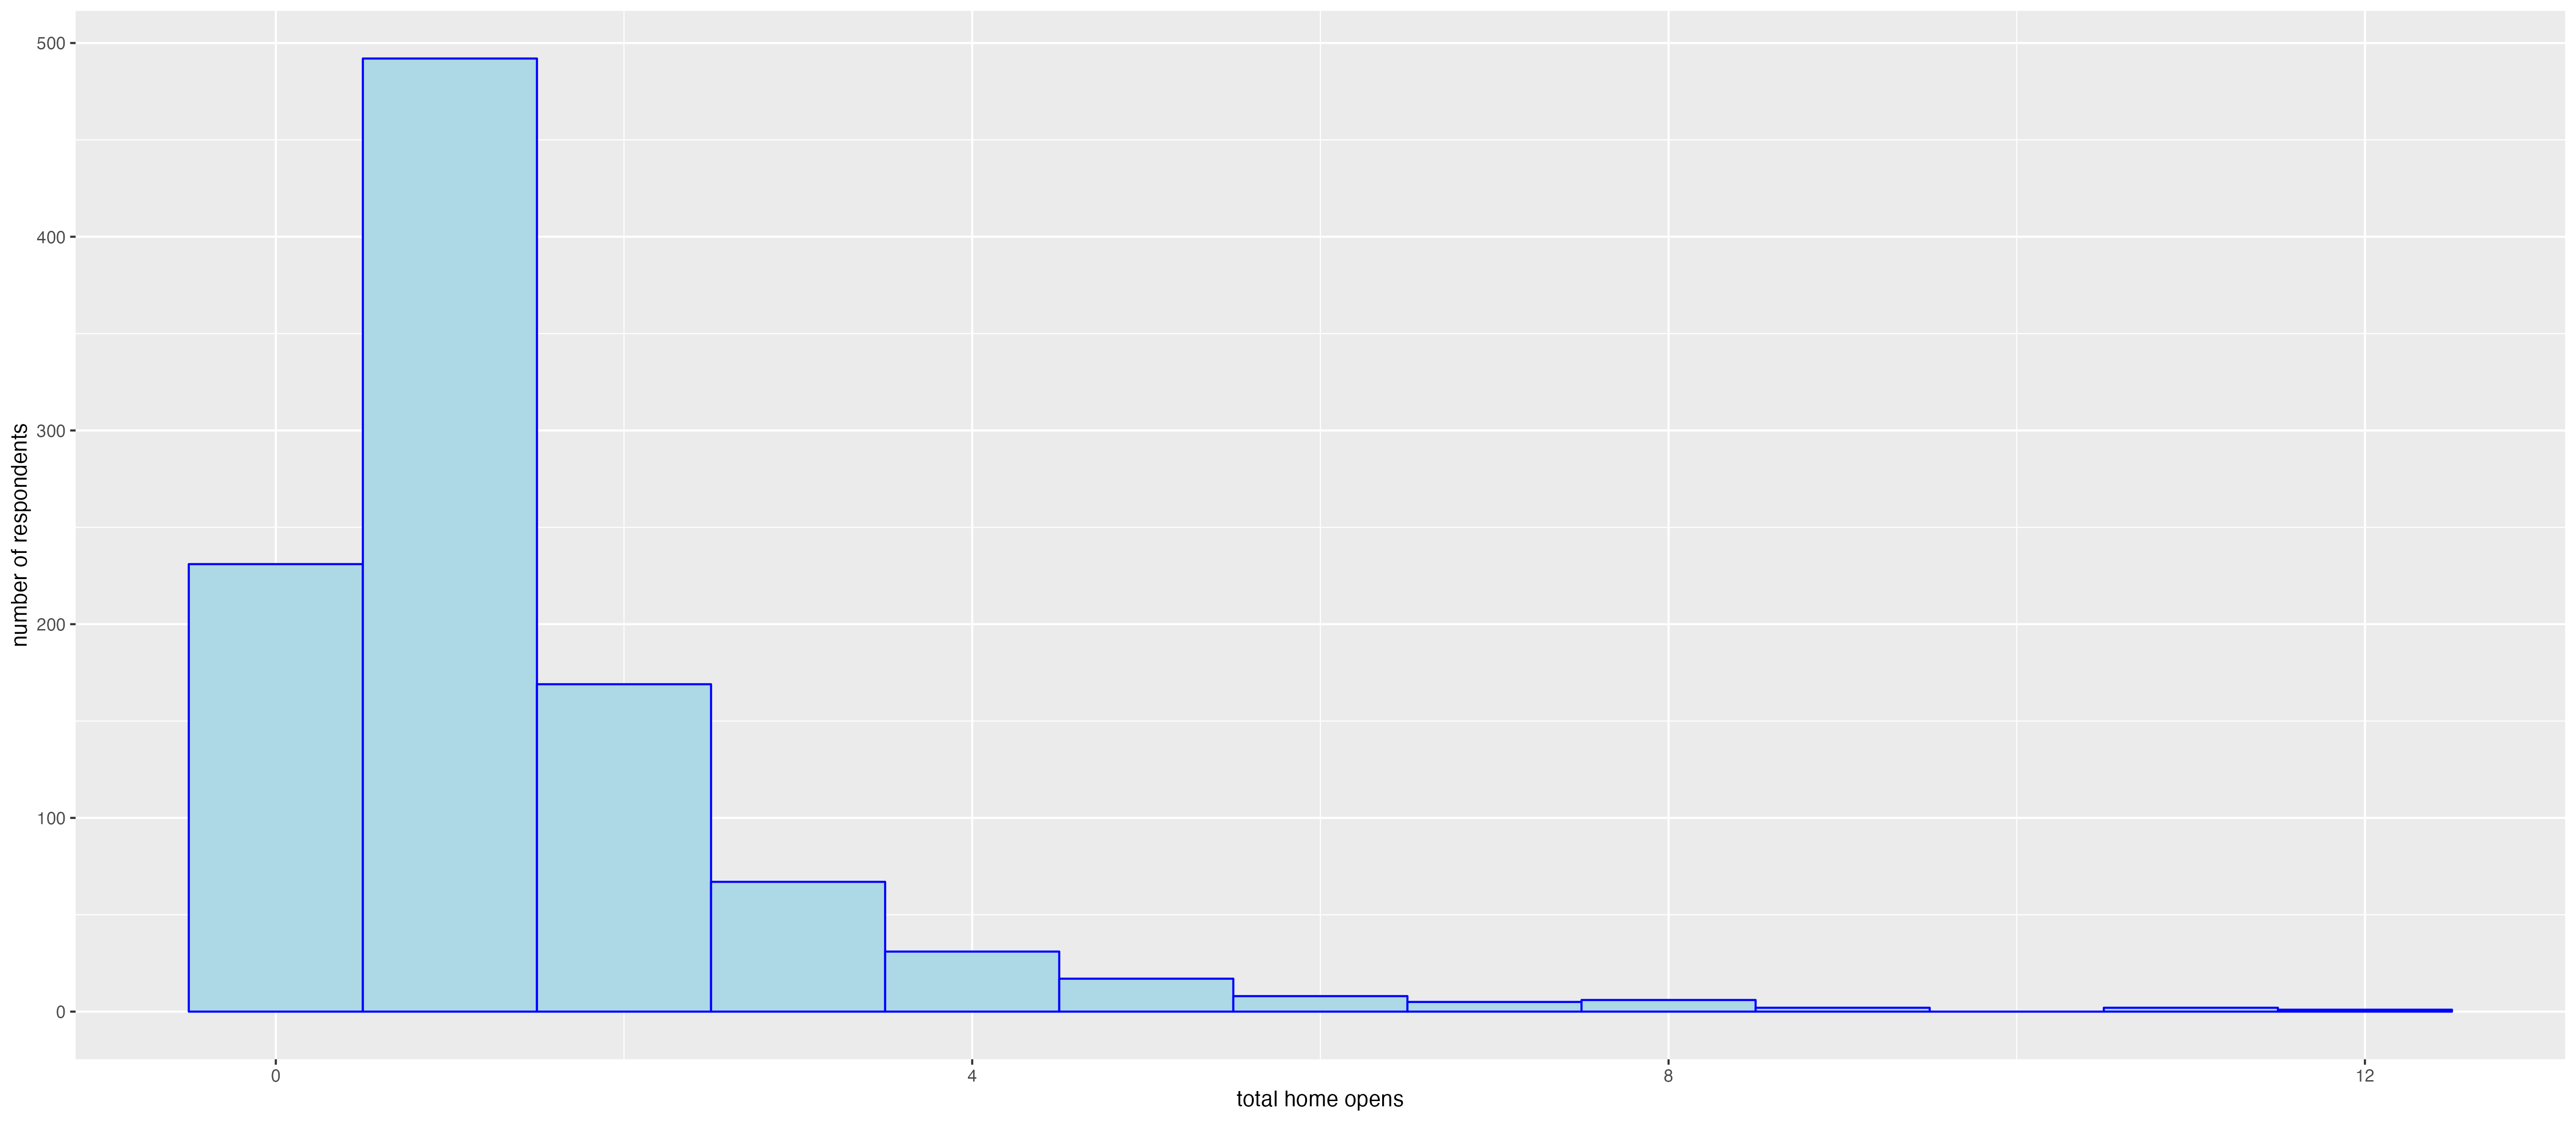
\includegraphics[scale=0.4]{app usage/plots/individual aggregates - home opens over lifetime.png}

% \subsubsection*{Number of home opens over time}
% The number of respondents who opened the app drops off steeply after week 1. 744 respondents filled had home open event logged in week 1 since treatment. 129 respondents had home open event logged in week 2.
% 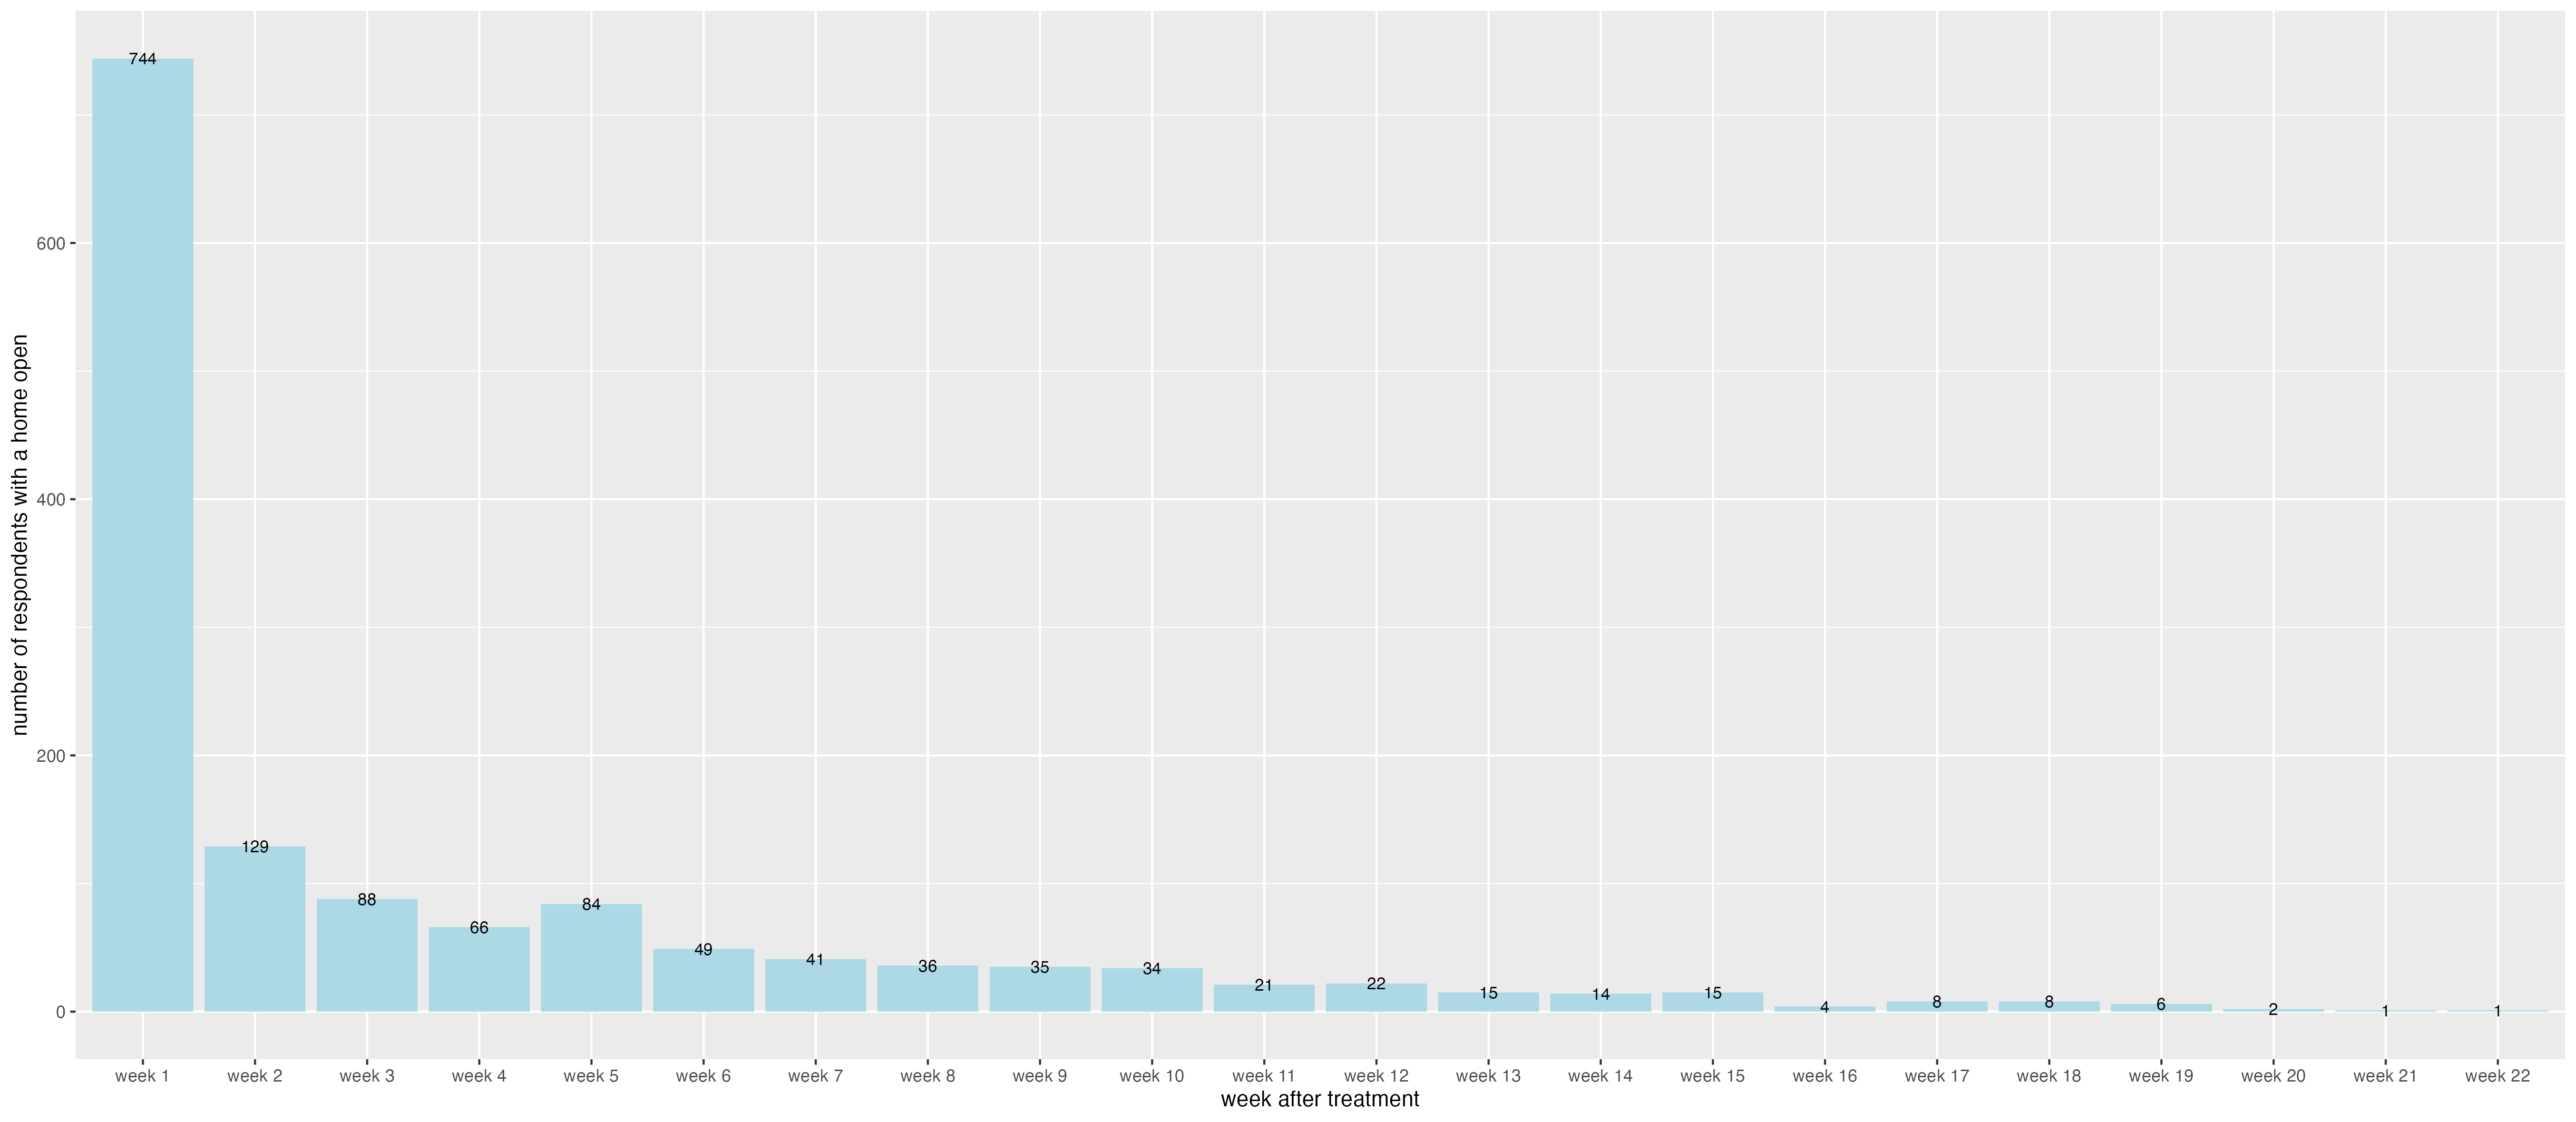
\includegraphics[scale=0.4]{app usage/plots/home opens over time - home opens.png}
% \end{figure}

% \begin{figure}
% \subsubsection*{Number of days used}
% We report the mean number of days of the week the respondent used the app. Respondents have app activity on 1 day in the week for most weeks. The text label annotates the number of respondents who opened any page of the app and contribute to the observations for that week.
% 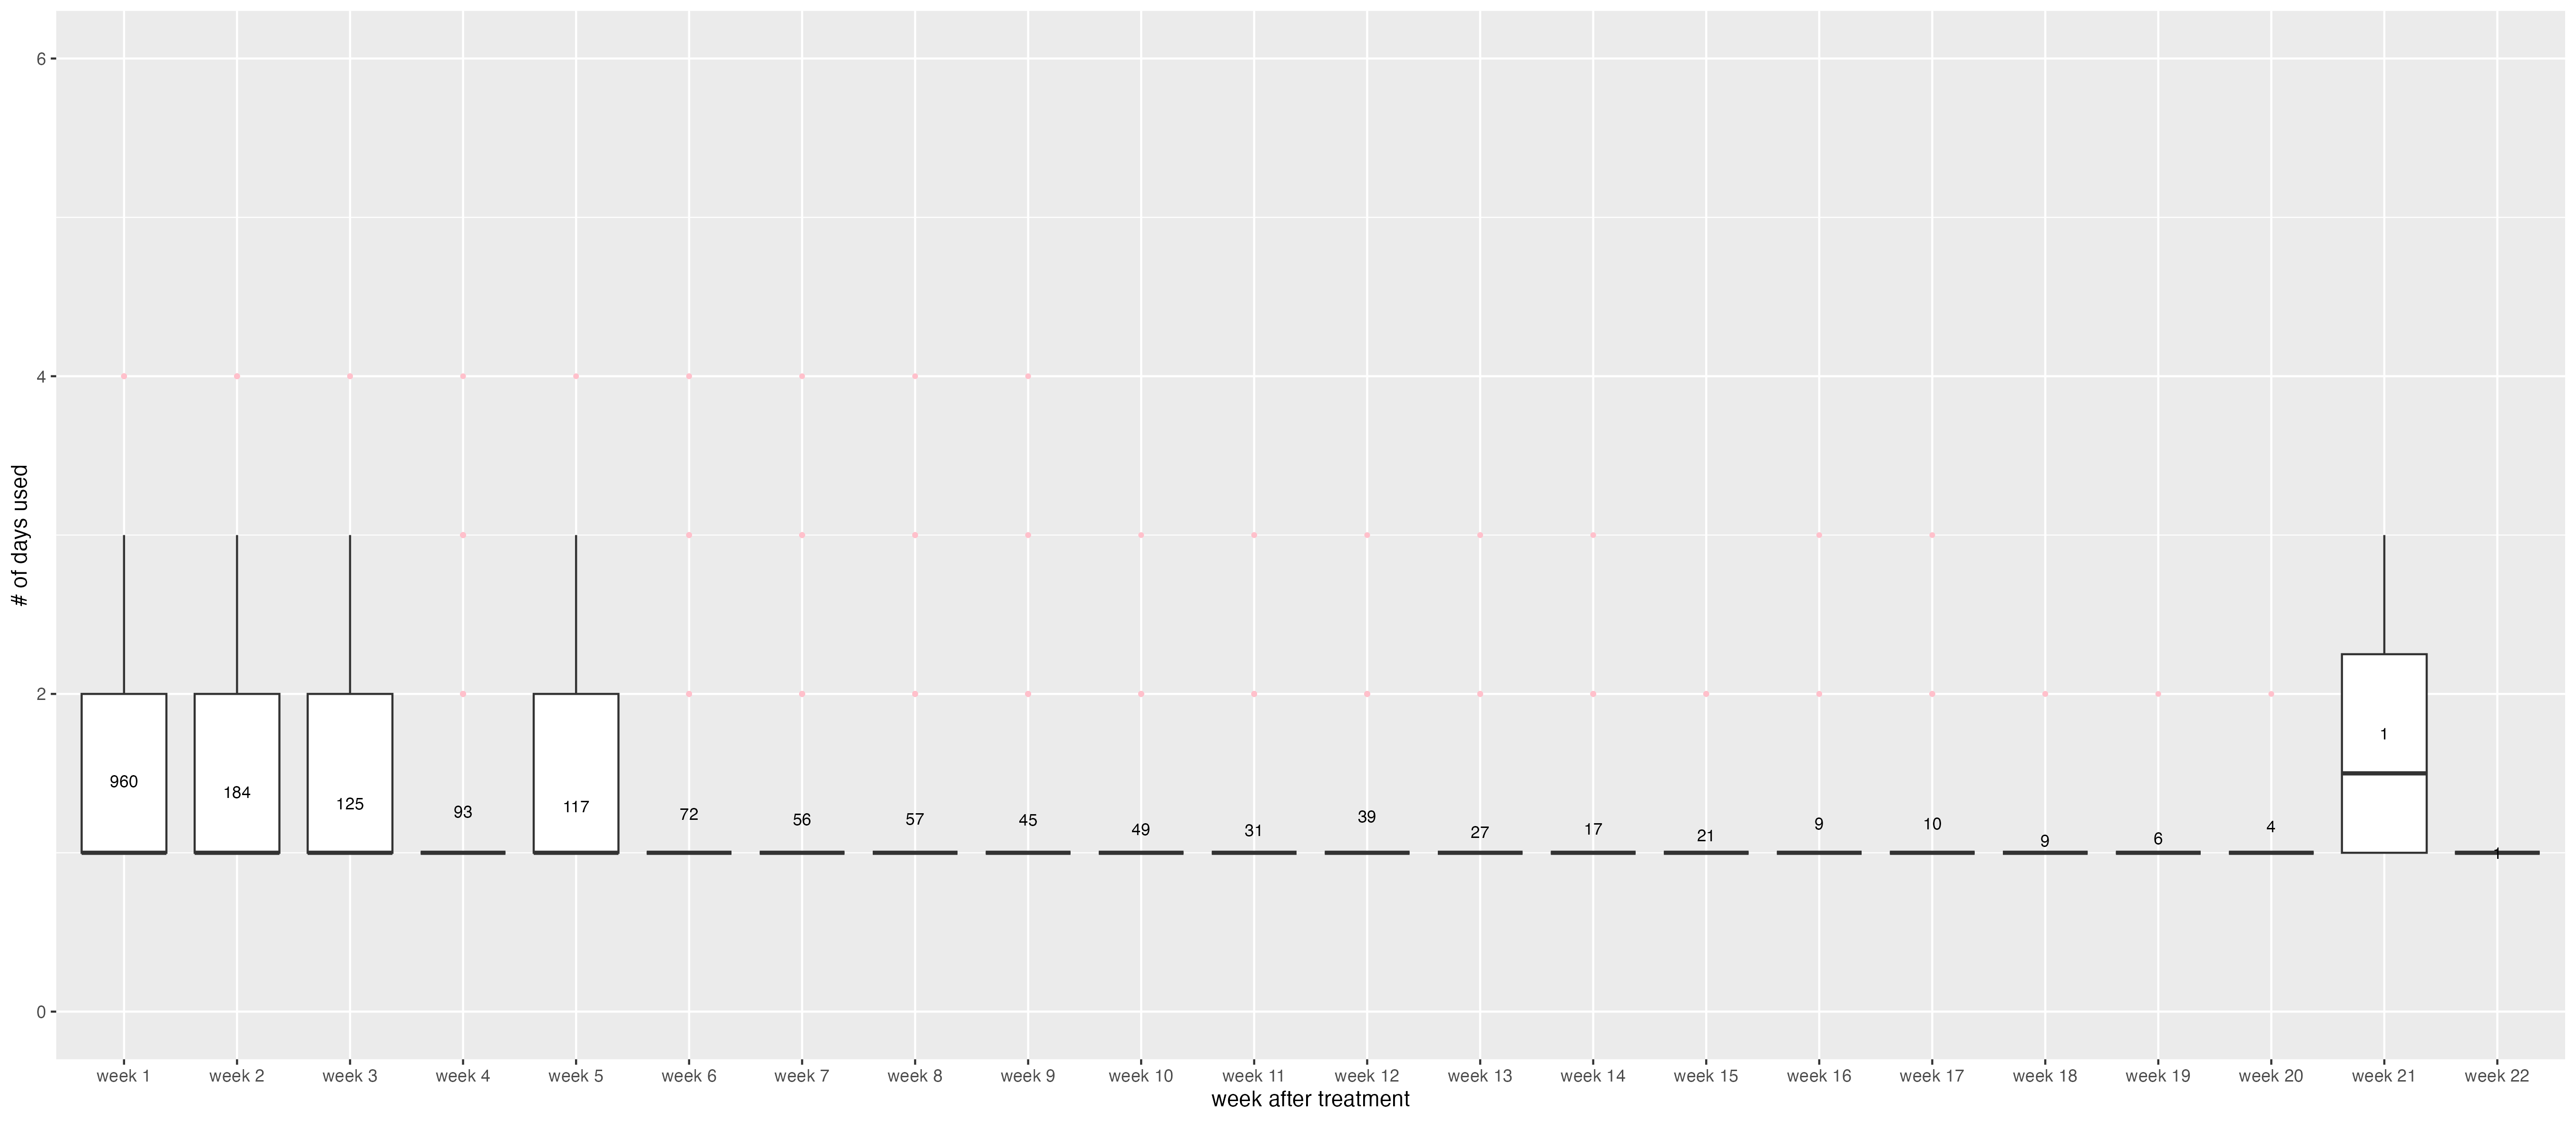
\includegraphics[scale=0.35]{app usage/plots/app usage over time - days used.png}

% \subsubsection*{Usage counts}
% We report the mean number of events logged for respondents for each week since treatment. The number of events logged drops steeply after week 1. The text label annotates the number of respondents who opened any page of the app and contributed to the observations for that week.
% 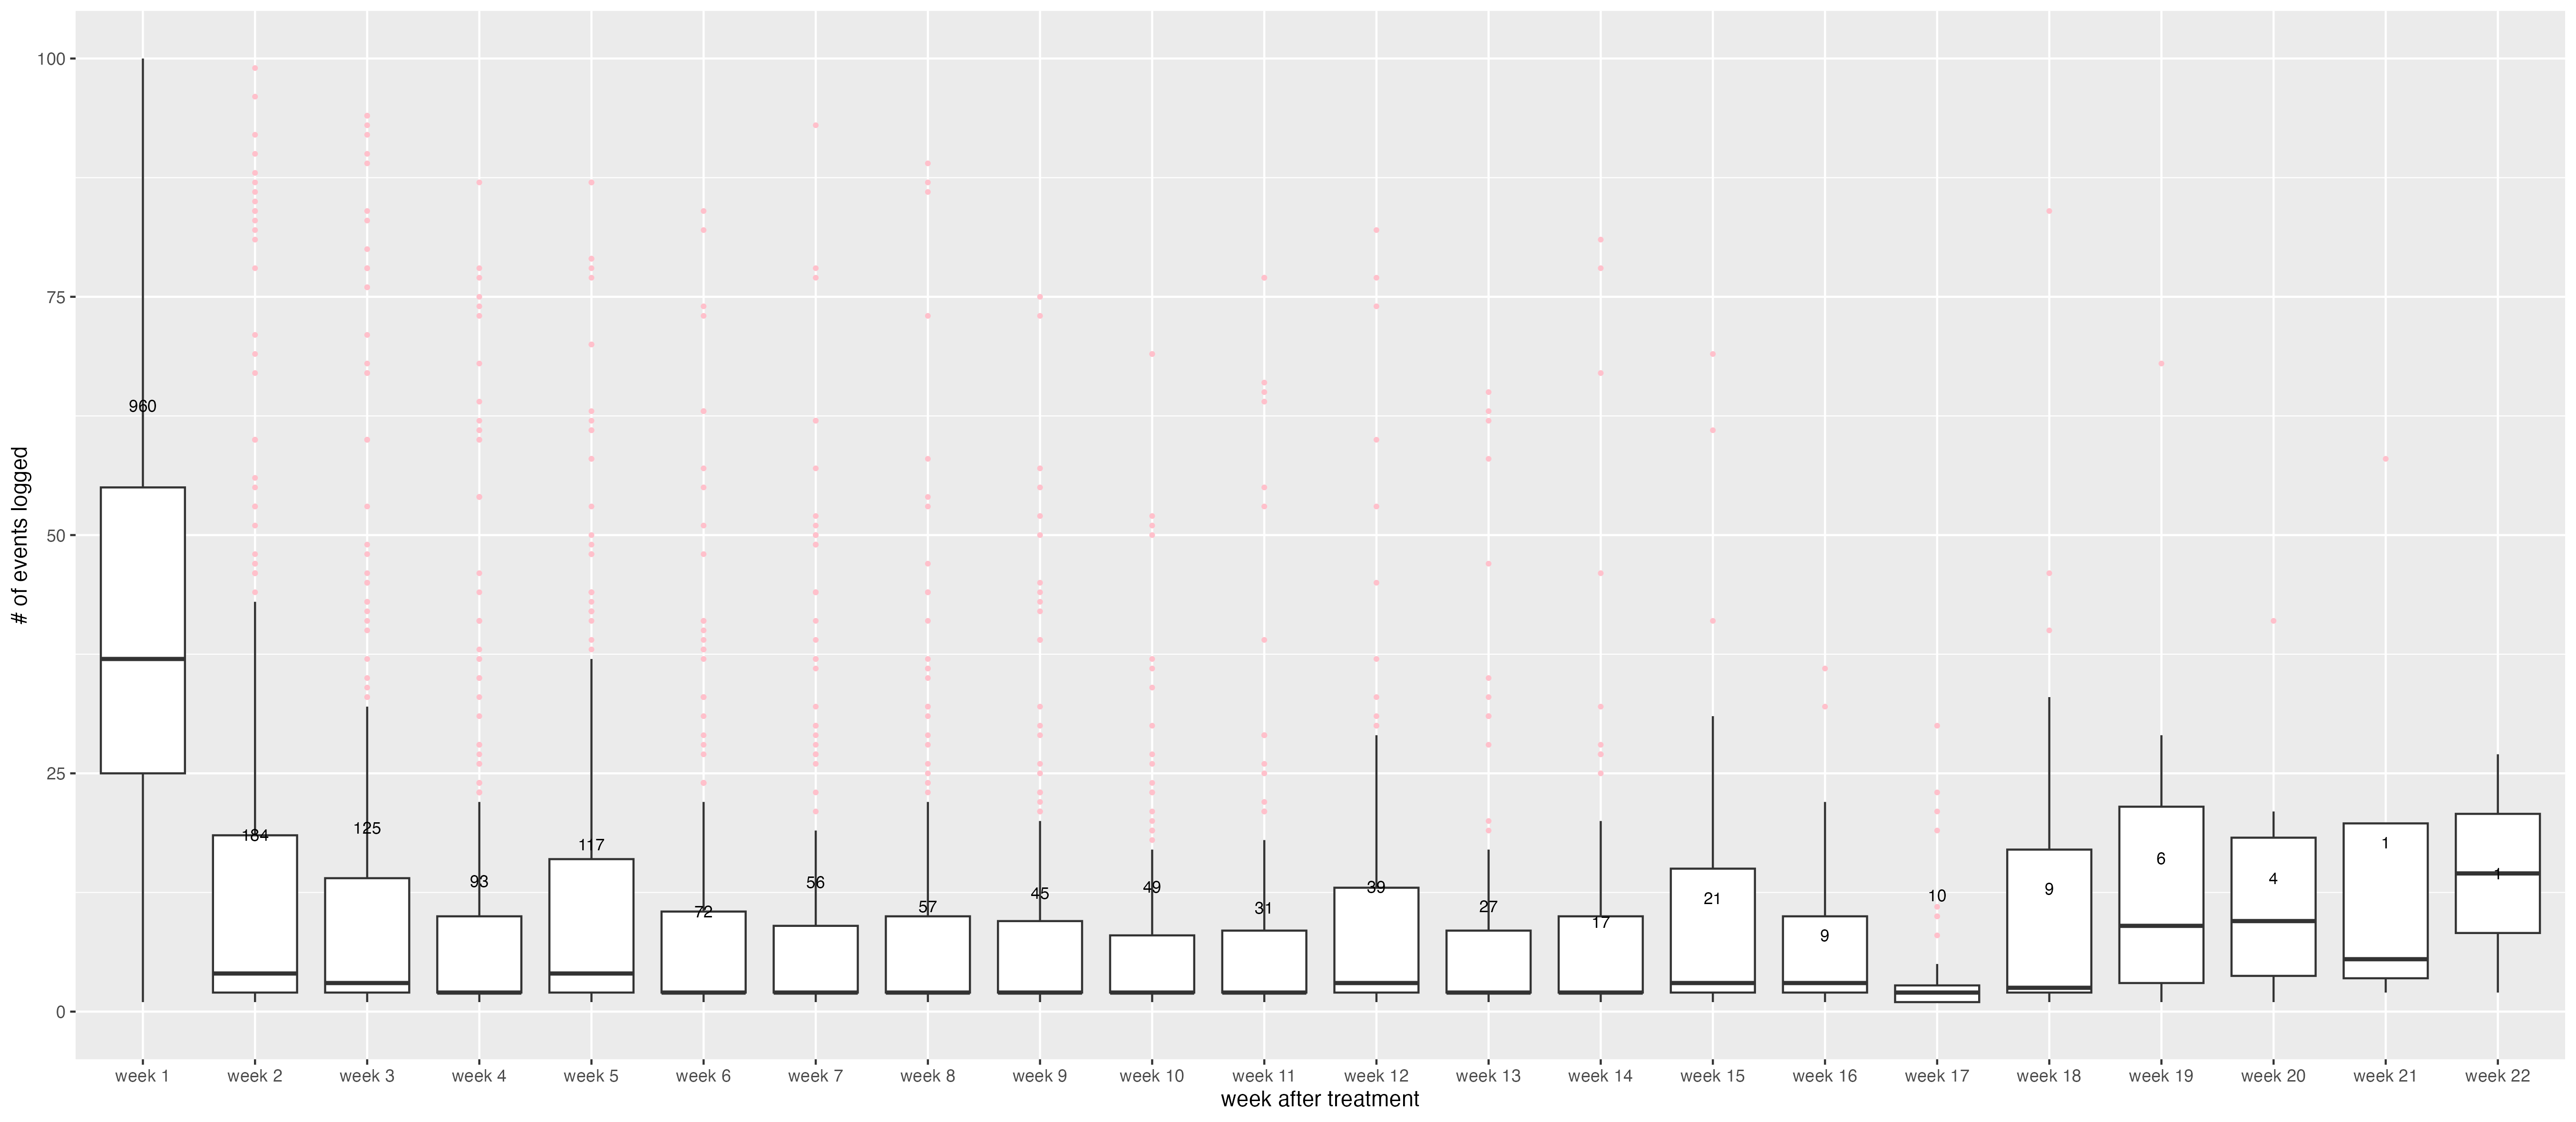
\includegraphics[scale=0.35]{app usage/plots/app usage over time - usage count.png}
% \end{figure}

% \begin{figure}
% \subsubsection*{Home opens}
% We report the mean number of home opens per respondent for each week since treatment. By week 4, the majority of respondents do not open the home page of the app except for some outliers. The text label annotates the number of respondents who opened any page of the app and contributed to the observations for that week.
% 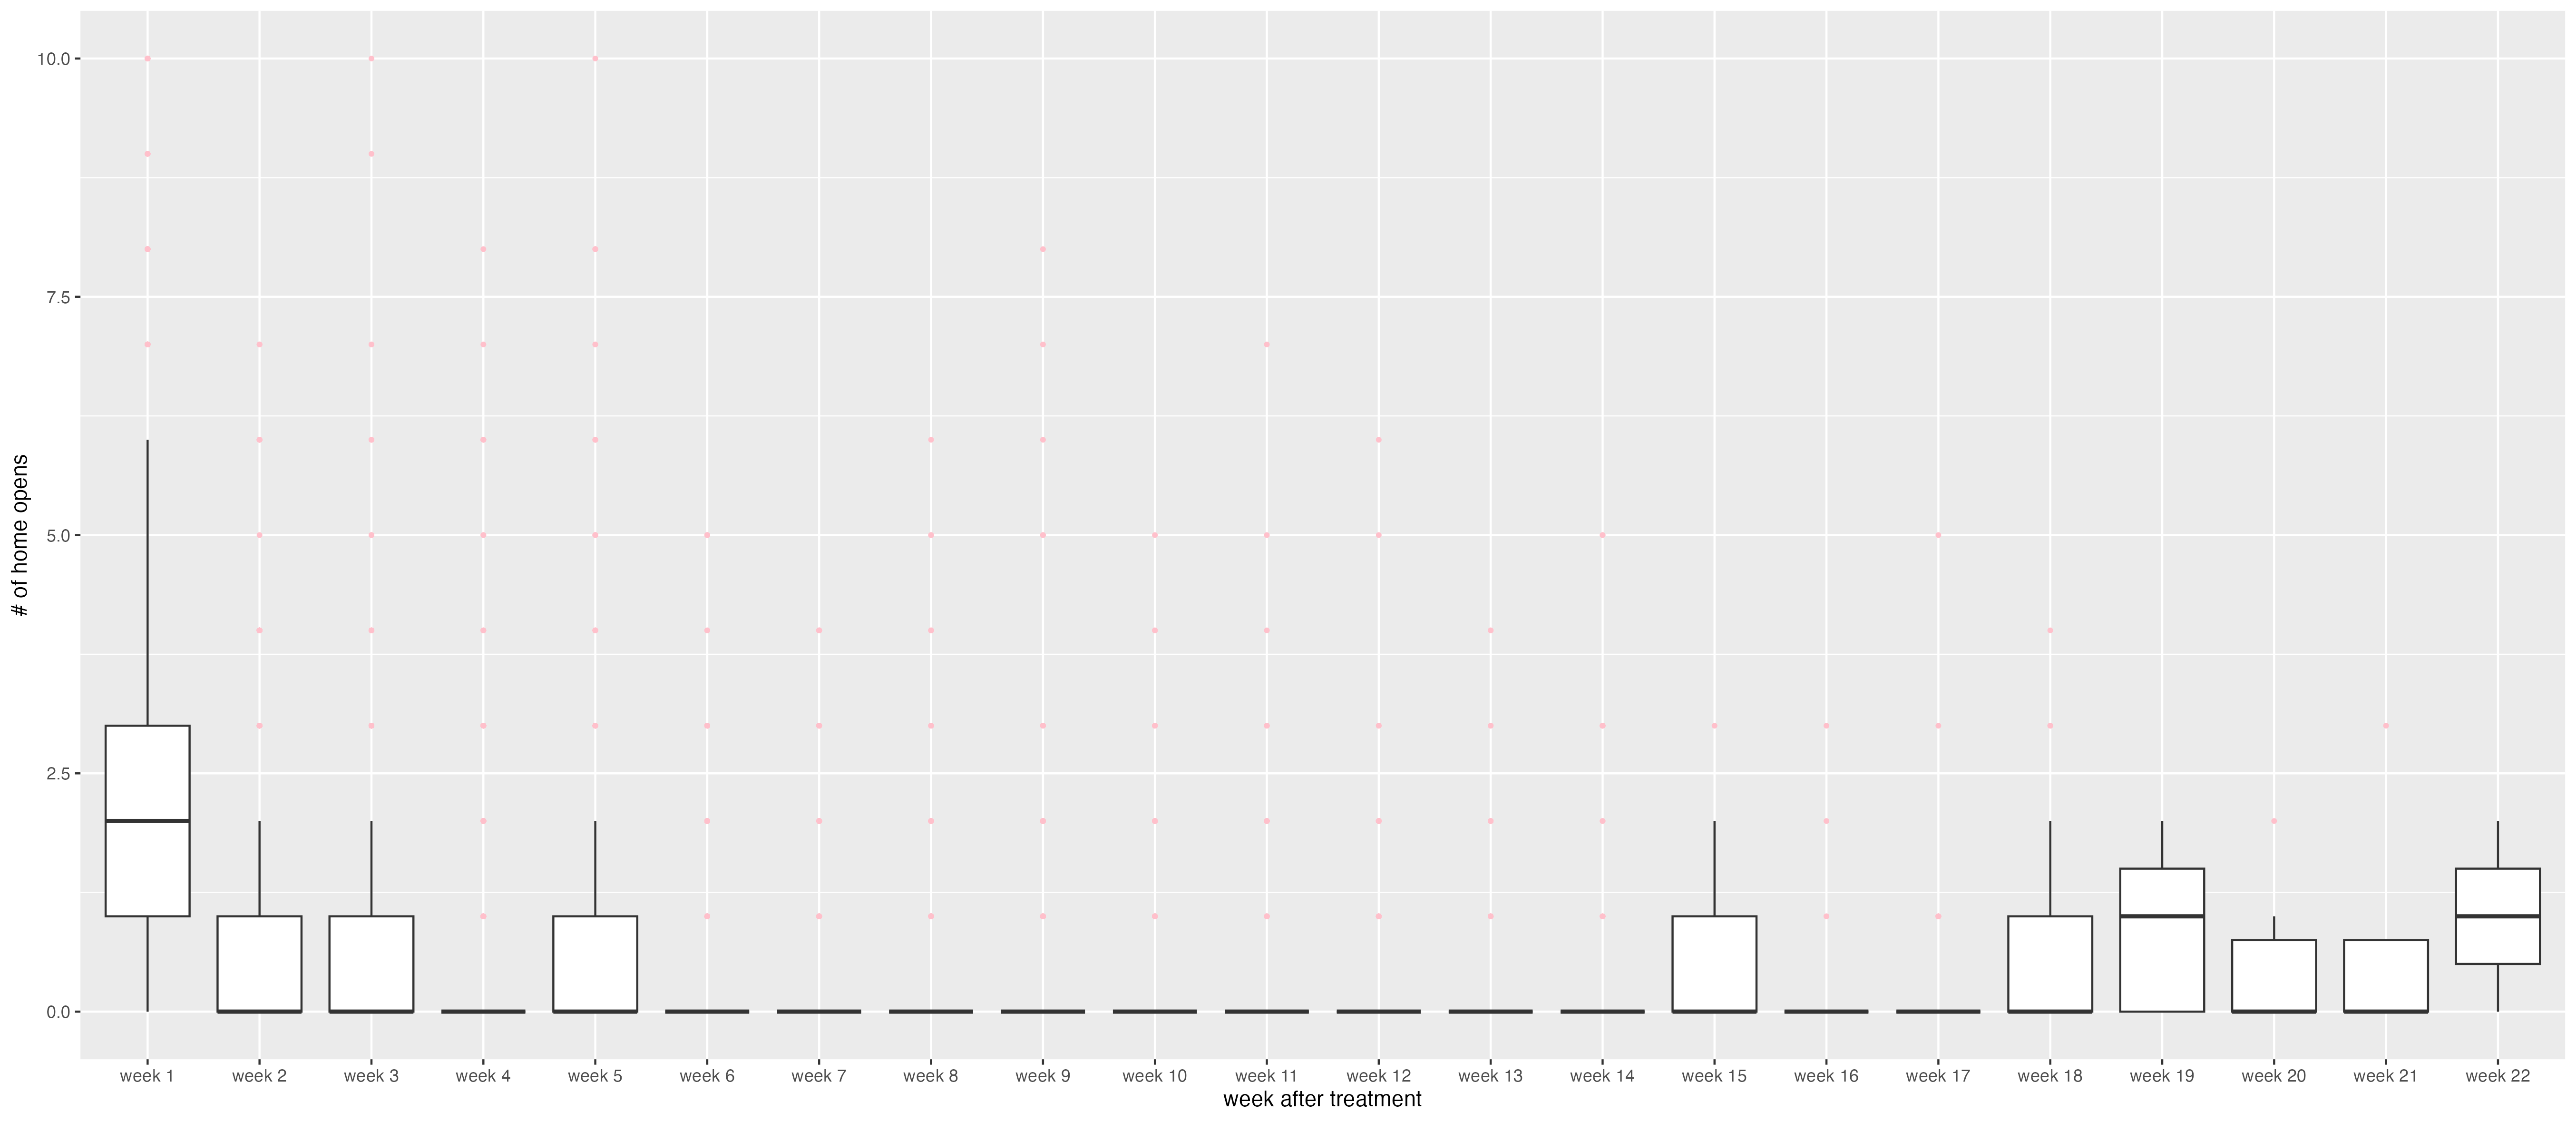
\includegraphics[scale=0.35]{app usage/plots/app usage over time - home opens.png}
% \end{figure}

% \addcontentsline{toc}{subsection}{App activity and user characteristics}
% \section*{App Activity and User Characteristics}

% In this analysis, we attempt to answer the questions -
% \begin{enumerate}
%     \item Who are the respondents who used the app?
%     \item Do more knowledgeable parents use the app more?
% \end{enumerate}

% We do so by regressing respondents' app usage activity against their characteristics.
% \vspace{1em}

% \textbf{Independent variables :}
% \begin{itemize}
%     \item \textbf{Baseline characteristics} - respondents' scores on the construct variables. We only use the construct variables that have sufficiently high internal consistency. We drop the constructs that are highly correlated with other constructs. We find $parent\_knw$ to be correlated with $caregiver\_well\_being$. We drop the construct with lower reliability $caregiver\_well\_being$.
%     \item Demographics variables - parents' age flag (categorical), university flag (binary), gender (categorical), and number of children (numeric)
%     \item Survey response variables - survey duration, start week, country flag
% \end{itemize}

% \textbf{Dependent variables :}
% \begin{itemize}
%     \item Home opened - binary variable indicating whether the respondent had a home opened event logged
%     \item Home opens - continuous count variable indicating the respondents' count of total home opens
% \end{itemize}


% \subsubsection*{Home Opens and User Characteristics}
% For respondents who downloaded the app, we regress their number of home opens against their baseline characteristics, demographic variables, and survey response variables. The $R^{2}$ for this model is 0.065. Note that the country flag is not significant which means that app usage does not differ significantly across the two countries after holding constant user characteristics (Table \ref{tbl:app usage and baseline characteristics - linear reg}).
% 
% Table created by stargazer v.5.2.3 by Marek Hlavac, Social Policy Institute. E-mail: marek.hlavac at gmail.com
% Date and time: Thu, Sep 21, 2023 - 00:32:36
\begin{table}[!htbp] \centering 
  \caption{# home opens predicted by baseline characteristics} 
  \label{tbl:app usage and baseline characteristics - linear reg} 
\begin{tabular}{@{\extracolsep{5pt}} ccccc} 
\\[-1.8ex]\hline 
\hline \\[-1.8ex] 
 & Estimate & Std. Error & t value & Pr(\textgreater \textbar t\textbar ) \\ 
\hline \\[-1.8ex] 
(Intercept) & $10.35$ & $1.79$ & $5.78$ & $0$ \\ 
start\_week & $$-$0.15$ & $0.03$ & $$-$4.35$ & $0$ \\ 
dev\_knw\_recog & $0.36$ & $0.59$ & $0.60$ & $0.55$ \\ 
confidence & $$-$0.31$ & $0.28$ & $$-$1.08$ & $0.28$ \\ 
attitude & $$-$0.07$ & $0.22$ & $$-$0.30$ & $0.76$ \\ 
caregiver\_well\_being & $$-$0.90$ & $0.34$ & $$-$2.64$ & $0.01$ \\ 
practices\_24 & $$-$2.23$ & $0.78$ & $$-$2.85$ & $0.005$ \\ 
practices\_agree & $0.31$ & $0.26$ & $1.19$ & $0.23$ \\ 
practices\_hostility & $0.31$ & $0.26$ & $1.19$ & $0.24$ \\ 
parent\_age & $$-$0.01$ & $0.02$ & $$-$0.82$ & $0.41$ \\ 
number\_children & $0$ & $0$ & $0.36$ & $0.72$ \\ 
parent\_genderWoman & $0.63$ & $0.45$ & $1.41$ & $0.16$ \\ 
survey\_duration & $0.09$ & $0.05$ & $1.82$ & $0.07$ \\ 
education & $0.02$ & $0.36$ & $0.04$ & $0.96$ \\ 
age\_flag2-6 & $$-$1.22$ & $0.34$ & $$-$3.55$ & $0$ \\ 
countryserbia & $$-$0.09$ & $0.58$ & $$-$0.15$ & $0.88$ \\ 
\hline \\[-1.8ex] 
\end{tabular} 
\end{table} 


% \subsubsection*{Home Opened and User Characteristics}
% For respondents who were treated, i.e., asked to download the Bebbo app, we fit a logistic regression model to whether the respondent had a home opened event logged using the respondents' baseline characteristics, demographic variables, and their survey response variables (Table \ref{tbl:downloads and baseline characteristics - logistic reg}). The goodness of fit measure used is the percentage improvement in deviance over the null deviance (pseudo $R^{2}$). The pseudo $R^{2}$ for this model is 0.03.
% 
% Table created by stargazer v.5.2.3 by Marek Hlavac, Social Policy Institute. E-mail: marek.hlavac at gmail.com
% Date and time: Thu, Sep 21, 2023 - 00:32:36
\begin{table}[!htbp] \centering 
  \caption{home opened (binary) predicted by baseline characteristics} 
  \label{tbl:home opened and baseline characteristics - logistic reg} 
\begin{tabular}{@{\extracolsep{5pt}} ccccc} 
\\[-1.8ex]\hline 
\hline \\[-1.8ex] 
 & Estimate & Std. Error & z value & Pr(\textgreater \textbar z\textbar ) \\ 
\hline \\[-1.8ex] 
(Intercept) & $1.11$ & $0.52$ & $2.15$ & $0.03$ \\ 
start\_week & $$-$0.04$ & $0.01$ & $$-$3.87$ & $0$ \\ 
dev\_knw\_recog & $0.31$ & $0.17$ & $1.84$ & $0.06$ \\ 
confidence & $$-$0.15$ & $0.08$ & $$-$1.89$ & $0.06$ \\ 
attitude & $0.01$ & $0.06$ & $0.22$ & $0.82$ \\ 
caregiver\_well\_being & $$-$0.20$ & $0.09$ & $$-$2.12$ & $0.03$ \\ 
practices\_24 & $$-$0.62$ & $0.22$ & $$-$2.77$ & $0.01$ \\ 
practices\_agree & $0.13$ & $0.07$ & $1.84$ & $0.07$ \\ 
practices\_hostility & $$-$0.10$ & $0.07$ & $$-$1.44$ & $0.15$ \\ 
parent\_age & $$-$0.02$ & $0.01$ & $$-$3.71$ & $0$ \\ 
number\_children & $0$ & $0$ & $0.24$ & $0.81$ \\ 
parent\_genderWoman & $0.31$ & $0.13$ & $2.47$ & $0.01$ \\ 
survey\_duration & $0.06$ & $0.01$ & $4.59$ & $0$ \\ 
education & $0.11$ & $0.10$ & $1.12$ & $0.26$ \\ 
age\_flag2-6 & $0.11$ & $0.10$ & $1.15$ & $0.25$ \\ 
countryserbia & $0.20$ & $0.16$ & $1.29$ & $0.20$ \\ 
\hline \\[-1.8ex] 
\end{tabular} 
\end{table} 


% \addcontentsline{toc}{section}{Attrition Analysis}
% \section*{Attrition}
% We define attrition as a respondent present in baseline but
% not present in endline. Attrition is indicated with a binary flag at the user level. For all respondents, we fit a logistic regression model to whether the respondent attrited using the respondents' baseline characteristics, demographic variables, and a flag for treatment (Table \ref{tbl:attrition and baseline characteristics - logistic reg}).

% \begin{itemize}
%     \item The goodness of fit measure used is the percentage improvement in deviance over the null deviance (pseudo $R^{2}$). The pseudo $R^{2}$ for this model is 0.95.
%     \item
% \end{itemize}
% 
% Table created by stargazer v.5.2.3 by Marek Hlavac, Social Policy Institute. E-mail: marek.hlavac at gmail.com
% Date and time: Thu, Sep 21, 2023 - 00:30:45
\begin{table}[!htbp] \centering 
  \caption{user attrition (binary) predicted by baseline characteristics} 
  \label{tbl:attrition and baseline characteristics - logistic reg} 
\begin{tabular}{@{\extracolsep{5pt}} ccccc} 
\\[-1.8ex]\hline 
\hline \\[-1.8ex] 
 & Estimate & Std. Error & z value & Pr(\textgreater \textbar z\textbar ) \\ 
\hline \\[-1.8ex] 
(Intercept) & $$-$1.47$ & $2.12$ & $$-$0.69$ & $0.49$ \\ 
treated & $129.00$ & $8,782.77$ & $0.01$ & $0.99$ \\ 
dev\_knw\_recog & $0.14$ & $0.70$ & $0.20$ & $0.84$ \\ 
confidence & $$-$0.41$ & $0.33$ & $$-$1.27$ & $0.20$ \\ 
attitude & $$-$0.23$ & $0.22$ & $$-$1.07$ & $0.28$ \\ 
caregiver\_well\_being & $0.02$ & $0.40$ & $0.06$ & $0.95$ \\ 
practices\_24 & $1.70$ & $1.17$ & $1.45$ & $0.15$ \\ 
practices\_agree & $$-$0.24$ & $0.33$ & $$-$0.72$ & $0.47$ \\ 
practices\_hostility & $0.35$ & $0.29$ & $1.20$ & $0.23$ \\ 
parent\_age & $0.001$ & $0.002$ & $0.38$ & $0.70$ \\ 
number\_children & $0$ & $0$ & $$-$0.01$ & $0.99$ \\ 
parent\_genderWoman & $$-$0.04$ & $0.53$ & $$-$0.07$ & $0.94$ \\ 
survey\_duration & $$-$0.26$ & $0.10$ & $$-$2.70$ & $0.01$ \\ 
education & $$-$0.79$ & $0.51$ & $$-$1.54$ & $0.12$ \\ 
age\_flag2-6 & $0.09$ & $0.43$ & $0.20$ & $0.84$ \\ 
countryserbia & $$-$1.26$ & $0.66$ & $$-$1.92$ & $0.05$ \\ 
\hline \\[-1.8ex] 
\end{tabular} 
\end{table} 


% We also fit a logistic regression model to whether the respondent attrited using the respondents' app usage (Table \ref{tbl:attrition and app usage - logistic reg}). This is fit only to the treated users who have app usage. The pseudo $R^{2}$ for this model is 0.007. A respondent's $usage\_count$ and $days\_used$ are weak signals of future attrition.

% 
% Table created by stargazer v.5.2.3 by Marek Hlavac, Social Policy Institute. E-mail: marek.hlavac at gmail.com
% Date and time: Thu, Sep 21, 2023 - 00:30:51
\begin{table}[!htbp] \centering 
  \caption{} 
  \label{tbl:attrition and app usage - logistic reg} 
\begin{tabular}{@{\extracolsep{5pt}} ccccc} 
\\[-1.8ex]\hline 
\hline \\[-1.8ex] 
 & Estimate & Std. Error & z value & Pr(\textgreater \textbar z\textbar ) \\ 
\hline \\[-1.8ex] 
(Intercept) & $2.70$ & $0.16$ & $16.85$ & $0$ \\ 
home\_opened & $$-$0.43$ & $0.39$ & $$-$1.11$ & $0.27$ \\ 
usage\_count & $$-$0.001$ & $0.001$ & $$-$1.77$ & $0.08$ \\ 
days\_used & $0.18$ & $0.09$ & $1.94$ & $0.05$ \\ 
downloaded & $0.26$ & $0.37$ & $0.69$ & $0.49$ \\ 
\hline \\[-1.8ex] 
\end{tabular} 
\end{table} 



% \addcontentsline{toc}{section}{Balance Tests}
% \section*{Balance Tests}

% % \addcontentsline{toc}{subsection}{Baseline vs Endline}
% % \subsection*{Baseline vs Endline}
% \addcontentsline{toc}{subsection}{Serbia vs Bulgaria}
% \subsection*{Testing for Baseline Imbalance by Country}
% \subsubsection*{Methodology}
% \begin{itemize}
%     \item We test for differences in the means between countries of all the survey question responses, construct variables and demographic variables.
%     \item We filter for baseline respondents who are also present in endline.
%     \item We run independent t-tests one at a time for each variable being tested.
%     \item We assume that the samples from both countries are being drawn from populations of equal variance.
% \end{itemize}

% 
% Table created by stargazer v.5.2.3 by Marek Hlavac, Social Policy Institute. E-mail: marek.hlavac at gmail.com
% Date and time: Thu, Sep 21, 2023 - 10:56:19
\begin{table}[!htbp] \centering 
  \caption{Baseline imbalance by country} 
  \label{tbl:country_baseline_constructs_imbalance} 
  \resizebox{\columnwidth}{!}{%
\begin{tabular}{@{\extracolsep{3pt}} ccccccccc} 
\\[-1.8ex]\hline 
\hline \\[-1.8ex] 
variable & serbia mean & bulgaria mean & test statistic & p-val & std.error & conf.int lower & conf.int upper & df \\ 
\hline \\[-1.8ex] 
health\_knw & 0.81 & 0.739 & 4.669 & 0 & 0.015 & 0.041 & 0.101 & 2074 \\ 
dev\_knw\_recog & 0.864 & 0.823 & 4.849 & 0 & 0.009 & 0.025 & 0.058 & 4855 \\ 
confidence & 3.392 & 3.256 & 7.056 & 0 & 0.019 & 0.098 & 0.174 & 4777 \\ 
attitude & 3.067 & 3.231 & -6.61 & 0 & 0.025 & -0.212 & -0.115 & 4739 \\ 
caregiver\_well\_being & 2.905 & 3.002 & -5.809 & 0 & 0.017 & -0.13 & -0.064 & 4724 \\ 
was\_breastfed & 0.405 & 0.298 & 4.801 & 0 & 0.022 & 0.064 & 0.152 & 1909 \\ 
practices\_24 & 0.839 & 0.784 & 8.809 & 0 & 0.006 & 0.043 & 0.068 & 4507 \\ 
practices\_agree & 2.94 & 1.421 & 71.916 & 0 & 0.021 & 1.478 & 1.56 & 4483 \\ 
practices\_hostility & 3.058 & 1.98 & 51.99 & 0 & 0.021 & 1.037 & 1.118 & 4465 \\ 
parent\_age & 31.704 & 31.039 & 3.055 & 0.002 & 0.218 & 0.238 & 1.092 & 8579 \\ 
 &  &  &  &  &  &  &  &  \\ 
\hline \\[-1.8ex] 
\end{tabular} %
}
\end{table} 


% \addcontentsline{toc}{subsection}{Treatment vs Control}
% \subsection*{Testing for Baseline Imbalance by Treatment}
% \subsubsection*{Methodology}

% \begin{itemize}
%     \item We test for differences in the means between treatment and control of all the survey question responses, construct variables, and demographic variables.
%     \item We filter for baseline respondents who are also present in endline.
%     \item We run independent t-tests one at a time for each variable being tested.
%     \item We assume that the samples from both countries are being drawn from populations of equal variance.
%     \item We repeat this analysis for both countries, Serbia and Bulgaria
% \end{itemize}

% 
% Table created by stargazer v.5.2.3 by Marek Hlavac, Social Policy Institute. E-mail: marek.hlavac at gmail.com
% Date and time: Mon, Sep 11, 2023 - 08:46:02
\begin{table}[!htbp] \centering 
  \caption{} 
  \label{tbl:treatment_baseline_imbalance_serbia} 
\begin{tabular}{@{\extracolsep{5pt}} cccccc} 
\\[-1.8ex]\hline 
\hline \\[-1.8ex] 
variable & test statistic & p-val & std.error & conf.int lower & conf.int upper \\ 
\hline \\[-1.8ex] 
multiplication & 2.769 & 0.006 & 0.024 & 0.02 & 0.115 \\ 
concern\_3yo & 2.412 & 0.016 & 0.029 & 0.013 & 0.127 \\ 
sort\_pair & -1.938 & 0.054 & 0.053 & -0.208 & 0.002 \\ 
know\_cog\_dev & 1.88 & 0.06 & 0.022 & -0.002 & 0.086 \\ 
dev\_knw\_concern\_3\_6 & 1.871 & 0.062 & 0.021 & -0.002 & 0.08 \\ 
simple\_songs & 1.67 & 0.096 & 0.029 & -0.008 & 0.104 \\ 
parent\_age & 1.545 & 0.123 & 0.491 & -0.205 & 1.724 \\ 
dev\_knw\_recog & 1.54 & 0.124 & 0.017 & -0.007 & 0.06 \\ 
concern\_5yo & 1.494 & 0.136 & 0.042 & -0.02 & 0.146 \\ 
scribble & 1.353 & 0.177 & 0.042 & -0.026 & 0.141 \\ 
sit\_support & 1.343 & 0.18 & 0.053 & -0.033 & 0.176 \\ 
know\_social\_emotional\_dev & 1.32 & 0.187 & 0.022 & -0.014 & 0.074 \\ 
past\_24h\_read & -1.227 & 0.22 & 0.027 & -0.087 & 0.02 \\ 
lose\_patience\_punish & -1.219 & 0.223 & 0.068 & -0.215 & 0.05 \\ 
express\_feelings & 1.104 & 0.271 & 0.045 & -0.039 & 0.139 \\ 
know\_phys\_dev & 1.055 & 0.292 & 0.02 & -0.018 & 0.061 \\ 
snap\_at\_child & 0.992 & 0.321 & 0.063 & -0.061 & 0.187 \\ 
past\_24h\_draw & -0.969 & 0.333 & 0.033 & -0.095 & 0.032 \\ 
know\_which\_vaccine & -0.86 & 0.39 & 0.047 & -0.133 & 0.052 \\ 
tell\_story & 0.855 & 0.393 & 0.028 & -0.031 & 0.078 \\ 
practices\_24 & -0.82 & 0.413 & 0.014 & -0.038 & 0.016 \\ 
concern\_12mo & -0.764 & 0.445 & 0.044 & -0.12 & 0.053 \\ 
health\_knw & -0.705 & 0.481 & 0.034 & -0.092 & 0.043 \\ 
make\_fun\_of & -0.684 & 0.494 & 0.066 & -0.176 & 0.085 \\ 
say\_name\_age & -0.632 & 0.528 & 0.049 & -0.128 & 0.066 \\ 
know\_lang\_dev & 0.625 & 0.532 & 0.021 & -0.028 & 0.055 \\ 
count\_to\_ten & 0.6 & 0.549 & 0.041 & -0.056 & 0.105 \\ 
parenting\_stress\_2 & 0.579 & 0.563 & 0.044 & -0.061 & 0.112 \\ 
cry\_separated & -0.52 & 0.604 & 0.04 & -0.1 & 0.058 \\ 
movement & 0.494 & 0.621 & 0.033 & -0.048 & 0.081 \\ 
past\_24h\_sing & 0.468 & 0.64 & 0.022 & -0.033 & 0.054 \\ 
past\_24h\_outside & -0.46 & 0.646 & 0.025 & -0.06 & 0.037 \\ 
know\_name\_age & 0.436 & 0.663 & 0.023 & -0.036 & 0.056 \\ 
name\_colors & 0.432 & 0.666 & 0.014 & -0.022 & 0.034 \\ 
practices\_hostility & -0.424 & 0.672 & 0.046 & -0.109 & 0.07 \\ 
breastfed & 0.251 & 0.802 & 0.054 & -0.093 & 0.12 \\ 
was\_breastfed & 0.251 & 0.802 & 0.054 & -0.093 & 0.12 \\ 
decrease\_stress & -0.235 & 0.815 & 0.029 & -0.063 & 0.049 \\ 
self\_care & -0.235 & 0.815 & 0.029 & -0.063 & 0.049 \\ 
know\_when\_vaccine & -0.232 & 0.817 & 0.035 & -0.076 & 0.06 \\ 
caregiver\_well\_being & 0.221 & 0.825 & 0.037 & -0.065 & 0.082 \\ 
confidence\_respond\_misbehave & -0.217 & 0.828 & 0.053 & -0.115 & 0.092 \\ 
threaten & -0.203 & 0.84 & 0.062 & -0.133 & 0.108 \\ 
joke\_with\_child & -0.194 & 0.846 & 0.071 & -0.154 & 0.126 \\ 
alphabet & 0.189 & 0.85 & 0.044 & -0.078 & 0.094 \\ 
physical\_punishment & 0.184 & 0.854 & 0.053 & -0.094 & 0.113 \\ 
attitude & 0.184 & 0.854 & 0.053 & -0.094 & 0.113 \\ 
parent\_knw & -0.181 & 0.856 & 0.046 & -0.099 & 0.082 \\ 
past\_24h\_play & 0.126 & 0.9 & 0.015 & -0.028 & 0.032 \\ 
past\_24h\_stories & -0.119 & 0.906 & 0.023 & -0.048 & 0.043 \\ 
smile\_around\_child & 0.114 & 0.909 & 0.07 & -0.129 & 0.145 \\ 
confidence\_deal\_emotions & -0.105 & 0.917 & 0.05 & -0.104 & 0.093 \\ 
parenting\_stress\_1 & 0.089 & 0.929 & 0.053 & -0.1 & 0.109 \\ 
personal\_needs & -0.082 & 0.935 & 0.057 & -0.116 & 0.106 \\ 
meaning\_of\_no & -0.081 & 0.935 & 0.044 & -0.09 & 0.083 \\ 
improve\_family & 0.075 & 0.94 & 0.032 & -0.06 & 0.064 \\ 
family\_care & 0.075 & 0.94 & 0.032 & -0.06 & 0.064 \\ 
play\_on\_floor & 0.041 & 0.968 & 0.071 & -0.136 & 0.141 \\ 
laugh\_together & 0.039 & 0.969 & 0.075 & -0.144 & 0.15 \\ 
dev\_knw\_concern\_0\_2 & 0.021 & 0.983 & 0.015 & -0.028 & 0.029 \\ 
practices\_agree & 0 & 1 & 0.055 & -0.108 & 0.108 \\ 
\hline \\[-1.8ex] 
\end{tabular} 
\end{table} 

% 
% Table created by stargazer v.5.2.3 by Marek Hlavac, Social Policy Institute. E-mail: marek.hlavac at gmail.com
% Date and time: Thu, Sep 21, 2023 - 10:56:02
\begin{table}[!htbp] \centering 
  \caption{} 
  \label{tbl:treatment_baseline_imbalance_bulgaria} 
\begin{tabular}{@{\extracolsep{5pt}} ccccccccc} 
\\[-1.8ex]\hline 
\hline \\[-1.8ex] 
variable & treatment mean & control mean & test statistic & p-val & std.error & conf.int lower & conf.int upper & df \\ 
\hline \\[-1.8ex] 
dev\_knw\_recog & 0.841 & 0.804 & 2.579 & 0.01 & 0.014 & 0.009 & 0.064 & 1863 \\ 
parent\_age & 31.333 & 30.721 & 1.685 & 0.092 & 0.363 & -0.1 & 1.325 & 3754 \\ 
practices\_24 & 0.791 & 0.776 & 1.433 & 0.152 & 0.011 & -0.006 & 0.036 & 1689 \\ 
attitude & 3.258 & 3.202 & 1.409 & 0.159 & 0.04 & -0.022 & 0.134 & 1804 \\ 
practices\_hostility & 1.999 & 1.961 & 1.158 & 0.247 & 0.033 & -0.026 & 0.102 & 1676 \\ 
confidence & 3.269 & 3.243 & 0.864 & 0.388 & 0.03 & -0.033 & 0.085 & 1826 \\ 
caregiver\_well\_being & 3.012 & 2.991 & 0.786 & 0.432 & 0.027 & -0.031 & 0.074 & 1797 \\ 
health\_knw & 0.748 & 0.729 & 0.772 & 0.441 & 0.025 & -0.03 & 0.068 & 829 \\ 
was\_breastfed & 0.286 & 0.31 & -0.739 & 0.46 & 0.033 & -0.09 & 0.041 & 747 \\ 
practices\_agree & 1.426 & 1.416 & 0.515 & 0.607 & 0.02 & -0.028 & 0.048 & 1681 \\ 
 &  &  &  &  &  &  &  &  \\ 
\hline \\[-1.8ex] 
\end{tabular} 
\end{table} 



\end{document}